\documentclass[11pt,a4paper,oneside]{book}
\usepackage[utf8]{inputenc}
\usepackage{graphicx}
\usepackage{hyperref}
\usepackage{amsmath}
\usepackage{amssymb}
\usepackage{geometry}
\usepackage{float}
\usepackage{tikz}
\usetikzlibrary{shapes,arrows,positioning,calc,fit}
\geometry{a4paper, margin=1in}

\title{\textbf{Computer Security}\\ \Large A Comprehensive Study Guide}
\author{Simone}
\date{2026}

\begin{document}

\maketitle

\frontmatter
\tableofcontents

\mainmatter

% Chapter 1: Introduction to Computer Security
\chapter{Introduction to Computer Security}
\label{ch:intro_security}

\section{Introduction}
Computer security is often perceived by the general public through the lens of dramatic media representations, but at its core, it is fundamentally an engineering problem. The discipline is driven by a few basic but profound questions: What constitutes a secure system? How do we define computer security? And, most importantly, how do we engineer systems to be secure?

\section{The CIA Paradigm: Basic Security Requirements}
To meaningfully discuss and measure security, the industry relies on a foundational model known as the \textbf{CIA Paradigm} (or CIA Triad). This model defines three primary security requirements that must be upheld to consider a system secure:

\begin{itemize}
    \item \textbf{Confidentiality (C):} This principle ensures that information can be accessed only by authorized entities. Confidentiality is what protects sensitive data, such as personal user information or intellectual property, from being exposed to those who should not have it.
    \item \textbf{Integrity (I):} Integrity guarantees that information can be modified only by authorized entities, and only in ways that they are explicitly permitted to do so. This prevents unauthorized tampering, ensuring that data remains accurate and trustworthy.
    \item \textbf{Availability (A):} Availability ensures that information and system resources must be available to all authorized parties within specified, acceptable time constraints. A system that is perfectly confidential and perfectly integral but completely inaccessible is virtually useless.
\end{itemize}

A significant challenge in engineering secure systems is that these properties often conflict. For instance, maximizing Availability (e.g., making a system accessible from anywhere, at any time) inherently increases the attack surface, putting Confidentiality and Integrity at risk. Conversely, aggressively locking down a system to preserve Confidentiality can severely hinder Availability. Balancing these trade-offs is the essence of security engineering.

\section{Security as an Engineering Problem}
Treating security as an engineering discipline means moving away from absolute statements (like ``this system is unhackable'') and towards a structured understanding of vulnerabilities, threats, and risks. No system is truly invulnerable; thus, the goal is to systematically manage and mitigate these aspects. To do so, several key concepts must be defined: vulnerabilities, exploits, assets, threats, and risks.

\subsection{Vulnerabilities vs. Exploits}
It is crucial to distinguish between a vulnerability and an exploit. 

A \textbf{Vulnerability} is a weakness or flaw in a system that allows an attacker to violate one or more of the constraints of the CIA paradigm. It is the underlying condition that \textit{can} be abused.

An \textbf{Exploit}, on the other hand, is a \textit{specific way} to use one or more vulnerabilities to accomplish a specific objective that violates those constraints. It is the active application of a technique against the vulnerability.

\subsubsection{Physical Security Example: Lock Picking}
Consider a physical lock protecting a vault. A standard pin-tumbler lock may have a mechanical vulnerability due to imperfect manufacturing tolerances. When rotational pressure (torque) is applied to the lock's plug, not all pins bind simultaneously; one pin will bind first due to microscopic size discrepancies. 

The exploit for this vulnerability is the technique of \textit{lock picking}. An attacker uses a \textbf{tension wrench} to apply continuous torque to the plug. They then use a \textbf{pick} to lift the pins one by one. Because of the binding friction, once a pin is lifted to the \textbf{shear line} (the gap between the plug and the lock housing), it stays caught there. By repeating this process for all pins, the attacker aligns the shear line, and the lock opens.

\begin{figure}[htpb]
\centering
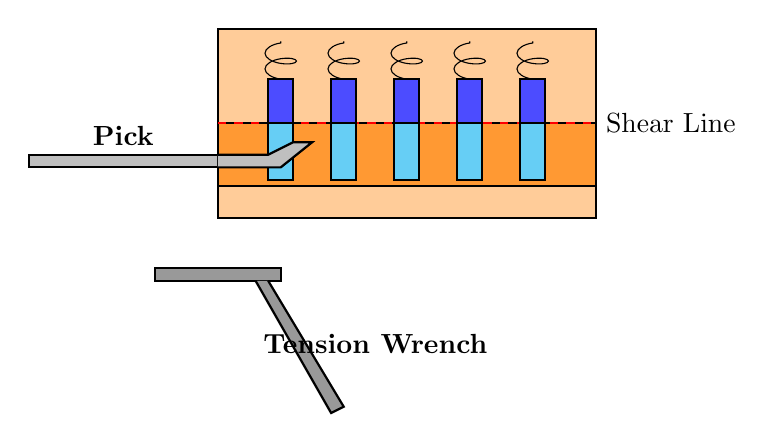
\begin{tikzpicture}[scale=0.8]
    % Outer housing
    \draw[fill=orange!40, thick] (0, 0) rectangle (6, 3);
    % Plug
    \draw[fill=orange!80, thick] (0, 0.5) rectangle (6, 1.5);
    
    % Shear line
    \draw[dashed, red, thick] (0, 1.5) -- (6, 1.5) node[right, text=black] {Shear Line};
    
    % Pins
    \foreach \x in {1, 2, 3, 4, 5} {
        % Bottom pin (key pin)
        \draw[fill=cyan!60, thick] (\x-0.2, 0.6) rectangle (\x+0.2, 1.5);
        % Top pin (driver pin)
        \draw[fill=blue!70, thick] (\x-0.2, 1.5) rectangle (\x+0.2, 2.2);
        % Spring
        \draw[decorate, decoration={coil, aspect=0.4, segment length=2mm, amplitude=2mm}] (\x, 2.2) -- (\x, 2.8);
    }
    
    % Pick tool
    \draw[fill=gray!50, thick] (-3, 0.8) rectangle (0, 1.0);
    \draw[fill=gray!50, thick] (0, 0.8) -- (1, 0.8) -- (1.5, 1.2) -- (1.2, 1.2) -- (0.8, 1.0) -- (0, 1.0);
    \node at (-1.5, 1.3) {\textbf{Pick}};
    
    % Tension Wrench
    \draw[fill=gray!80, thick] (-1, -1) rectangle (1, -0.8);
    \draw[fill=gray!80, thick] (0.8, -1) -- (2, -3) -- (1.8, -3.1) -- (0.6, -1);
    \node at (2.5, -2) {\textbf{Tension Wrench}};
    
\end{tikzpicture}
\caption{Simplified illustration of exploiting a physical lock. The tension wrench applies torque, creating binding friction. The pick lifts the pins to the shear line, exploiting mechanical tolerances (the vulnerability).}
\label{fig:lock_picking}
\end{figure}

To mitigate this, higher-quality locks introduce countermeasures like \textit{spool pins}, \textit{mushroom pins}, or \textit{serrated pins}. These do not eliminate the vulnerability entirely---the lock can still be picked---but they remove the feedback the attacker relies on, making the exploitation significantly more difficult and time-consuming.

\subsubsection{Software Security Example: Integer Truncation}
Software vulnerabilities often arise from seemingly innocuous programming mistakes. Consider the following simplified C code designed to authenticate a user based on an input number:

\begin{verbatim}
int i;
unsigned short s;

i = atoi(argv[1]); // parse command line parameter as int

if (i == 0) { // check
    printf("Invalid number: value must be > 0\n");
    return -1;
}

s = i; // implicit truncation

if (s == 0) { // security check
    printf("Access GRANTED!\n");
}
\end{verbatim}

\textbf{The Vulnerability:} The code validates the integer \texttt{i} to ensure it is not zero. In standard C, an \texttt{int} is typically 32 bits, while an \texttt{unsigned short} is only 16 bits. When \texttt{i} is assigned to \texttt{s}, the 32-bit integer is implicitly truncated to its lower 16 bits. The vulnerability is the combination of this unsafe type conversion and the subsequent security check relying on the truncated value.

\textbf{The Exploit:} An attacker can input a number that is not zero in 32 bits but becomes zero when truncated to 16 bits. Since $2^{16} = 65536$, running the program with the argument \texttt{65536} bypasses the first check (since $65536 \neq 0$). During the assignment \texttt{s = i}, the value \texttt{65536} (which in binary is a \texttt{1} followed by sixteen \texttt{0}s) is truncated. The lower 16 bits are all zero, so \texttt{s} becomes \texttt{0}. The final check \texttt{if (s == 0)} evaluates to true, and access is granted. Here, the number \texttt{65536} is the specific exploit.

\subsection{Assets, Threats, and Attacks}
To understand risk, we must map out what we are trying to protect and who we are protecting it from.

An \textbf{Asset} identifies what is valuable to an organization. In IT contexts, this includes:
\begin{itemize}
    \item \textbf{Hardware:} Laptops, servers, networking equipment.
    \item \textbf{Software:} Operating systems, custom applications, databases.
    \item \textbf{Data:} Customer records, intellectual property, financial ledgers.
    \item \textbf{Reputation:} The organization's standing, particularly regarding social media and public trust.
\end{itemize}

A \textbf{Threat} is a potential violation of the CIA paradigm---a circumstance or event capable of causing harm. Examples include Denial of Service (compromising Availability), Identity Theft (compromising Confidentiality/Integrity), or Data Leaks.

An \textbf{Attack} is the \textit{intentional} use of one or more exploits with the objective of compromising a system's CIA. For example, attaching a malicious PDF to an email or physically picking a lock to enter a server room.

A \textbf{Threat Agent} is the entity---whoever or whatever---that may cause an attack to occur, such as a malicious script, a rogue employee, or a physical thief.

\subsection{Demystifying Terminology: Hackers vs. Attackers}
The mass media has generated considerable confusion around security terminology. It is important to distinguish between these concepts.

An \textbf{Attacker} is anyone or anything that performs an attack.

A \textbf{Hacker}, historically and within the technical community, is someone with an \textit{advanced understanding} of computers and computer networks, driven by a deep willingness to learn ``everything'' about how systems work under the hood. 

An attacker is not necessarily a hacker (e.g., someone running a pre-packaged script without understanding it), and a hacker is not necessarily an attacker. When hackers use their skills maliciously, they are referred to as \textbf{Black Hats}. Conversely, \textbf{Security Professionals} or \textbf{White Hats} are ethical hackers. They use the same advanced skillset to:
\begin{itemize}
    \item Identify vulnerabilities.
    \item Develop exploits (to prove vulnerabilities exist).
    \item Develop attack-detection methods.
    \item Develop countermeasures.
    \item Engineer robust security solutions.
\end{itemize}

\section{Security as Risk Management}
Because no system is invulnerable, security cannot be treated as an absolute state. Instead, it is an exercise in \textbf{Risk Management}. 

\textbf{Risk} is defined as the statistical and economical evaluation of the exposure to damage resulting from the presence of vulnerabilities and threats. It can be conceptually modeled as:

\[ \text{Risk} = \text{Asset} \times \text{Vulnerabilities} \times \text{Threats} \]

In this equation:
\begin{itemize}
    \item \textbf{Threats} are generally an \textit{independent variable}. An organization usually cannot control whether malicious actors decide to target them.
    \item \textbf{Assets} and \textbf{Vulnerabilities} are \textit{controllable variables}. An organization decides what assets to put online and how rigorously to patch and secure them.
\end{itemize}

A highly vulnerable system facing zero threats might have a low overall risk, while a reasonably secure system facing persistent, advanced threats might have a high risk.

\subsection{The Balance of Security vs. Cost}
Engineering security means reducing vulnerabilities and planning for damage containment, but this must always be balanced against \textbf{cost}. Throwing more money at a problem does not inherently yield more security. For example, a highly expensive but improperly configured firewall provides a false sense of security and is arguably worse than having no firewall.

Costs are categorized into:
\begin{itemize}
    \item \textbf{Direct Costs:} Management overhead, operational expenses, and equipment purchases.
    \item \textbf{Indirect Costs (often more relevant):} Decreased usability, slower system performance, reduced user privacy due to invasive monitoring, and reduced overall productivity.
\end{itemize}

If security controls are too expensive in terms of usability (e.g., overly complex password policies requiring frequent changes), users will inevitably circumvent them (e.g., by writing passwords on sticky notes), effectively nullifying the security investment.

\section{Trust and Assumptions}
At the foundation of any secure system, boundaries must be set. Within these boundaries, certain elements must simply be \textit{assumed} secure. These form the \textbf{trusted elements} of the system. 

When evaluating a system, we must ask: Can we trust the security officer? The newly installed software? Our own code? The compiler? The BIOS? The hardware itself?

This creates a ``chicken and egg'' chain-of-trust problem. This paradox was famously explored by Ken Thompson in his 1984 Turing Award lecture, \textit{"Reflections on Trusting Trust"}. Thompson demonstrated how a compiler could be modified to insert a backdoor into programs it compiled (like the \texttt{login} command), and further, how the compiler could recognize when it was compiling \textit{itself} and insert the backdoor-generation code into the newly compiled compiler. The malicious source code could then be removed from the compiler's source tree, leaving no trace, yet the binary compiler would perpetually reproduce the vulnerability. This highlights that unless you bootstrap an entire system yourself from basic principles (as initiatives like \texttt{bootstrappable.org} attempt to do), you are ultimately placing blind trust in some foundational level of the technology stack.

\section{Conclusions}
Computer security is a complex engineering discipline focused on balancing conflicting requirements (Confidentiality, Integrity, Availability) against practical limitations and costs. It requires a nuanced understanding of risk management, where vulnerabilities must be weighed against actual threats and the value of the underlying assets. Recognizing the distinction between vulnerabilities and exploits, and between malicious attackers and skilled hackers, is crucial for developing effective countermeasures. Ultimately, because absolute security is unattainable and trust must invariably be placed somewhere in the supply chain, security remains an ongoing process of risk mitigation rather than a solvable destination.


% Chapter 2: Introduction to Cryptography
\chapter{Introduction to Cryptography}
\label{ch:introduction_to_cryptography}

Cryptography, historically referred to as cryptology, is fundamentally the study of mathematical techniques and protocols designed to enable secure communication and data storage in the presence of malicious adversaries. In modern computer security, cryptography provides the foundational primitives upon which secure systems are built.

\section{The Core Goals of Cryptography}

The application of cryptographic algorithms is intended to provide one or more of the following security features:
\begin{itemize}
    \item \textbf{Confidentiality}: Ensuring that data is accessible only to chosen, authorized entities. It prevents unauthorized parties from understanding the information even if they can intercept it.
    \item \textbf{Integrity and Freshness}: Detecting and preventing unauthorized tampering with data. Freshness is a temporal extension of integrity, preventing attackers from recording a legitimate, secure message and replaying it later (a replay attack).
    \item \textbf{Authenticity}: Certifying the origin of the data. It provides assurance that the data was indeed generated by the claimed sender.
    \item \textbf{Non-repudiation}: Establishing a mechanism where the creator of a piece of data cannot subsequently repudiate (deny) having created or sent it. This is vital for digital contracts and financial transactions.
    \item \textbf{Advanced Features}: Modern cryptography also explores complex functionalities such as proofs of knowledge or computation (e.g., zero-knowledge proofs), where a party can prove a statement is true without revealing the underlying data.
\end{itemize}

\section{A Brief Historical Perspective}

Cryptography is as old as written communication itself, originally born out of commercial needs (such as protecting the recipe for lacquer on clay tablets) and military applications (such as the Spartan scytale). For millennia, cryptographic algorithms were designed by humans to be computed by hand, using pen and paper.

\subsection{The Ancient View: A Battle of Wits}
Historically, cryptography was perceived as a continuous battle of wits between cryptographers, who ideated secret methods to obfuscate text, and cryptanalysts, who attempted to figure out the method and break the "cipher." A significant paradigm shift occurred in 1553 when Giovan Battista Bellaso separated the encryption method from the key. This meant the security of the message began to rely on a secret parameter rather than an obscure algorithm.

This concept was formalized centuries later by Auguste Kerckhoffs in 1883, who established six principles for a good cipher. The most famous, Kerckhoffs's Principle, states that a cryptographic system should be secure even if everything about the system, except the key, is public knowledge. Other principles emphasized practicality, such as the system being portable, applicable to telegraphic communication, and not imposing an excessive mental load on the operator.

\subsection{The Modern Era: From Machines to Mathematics}
The advent of mechanical computation drastically changed cryptography. The first rotor machine was invented by Edward Hebern in 1917, and the design was popularized during World War II by the German Enigma machine. The decisive cryptanalytic efforts at Bletchley Park, led by figures like Alan Turing, underscored the importance of algorithmic analysis and computation in breaking ciphers.

Following the war, cryptography transitioned from an ad-hoc battle of wits to a rigorous mathematical discipline. In 1949, Claude Shannon published "Communication Theory of Secrecy Systems," proving that mathematically unbreakable ciphers do exist. In 1955, John Nash argued that computationally secure ciphers are practically sufficient. Nash hypothesized that if the parts of a key interact complexly enough during encryption, the computational gap between the legitimate user (who takes polynomial time to encrypt/decrypt) and the attacker (who faces exponential time to break it) would become insurmountable.

\section{Fundamental Definitions and Information Theory}

Before delving into modern cryptographic constructions, we must formally define the components of a cryptosystem and understand how to measure information and uncertainty.

\subsection{Cryptographic Primitives and Spaces}
A cryptosystem operates over three primary sets:
\begin{itemize}
    \item \textbf{Plaintext space $\mathbf{P}$}: The set of all possible messages. In modern times, this is a set of bitstrings $\{0,1\}^l$.
    \item \textbf{Ciphertext space $\mathbf{C}$}: The set of all possible encrypted messages, $\text{ctx} \in \mathbf{C}$. Typically $\{0,1\}^{l'}$, where $l'$ may be greater than or equal to $l$.
    \item \textbf{Key space $\mathbf{K}$}: The set of all possible keys. Keys are usually binary strings $\{0,1\}^\lambda$, sometimes parsed into specific formats.
\end{itemize}

The system defines two deterministic functions:
\begin{itemize}
    \item \textbf{Encryption Function $\mathbb{E}$}: $\mathbf{P} \times \mathbf{K} \rightarrow \mathbf{C}$
    \item \textbf{Decryption Function $\mathbb{D}$}: $\mathbf{C} \times \mathbf{K} \rightarrow \mathbf{P}$
\end{itemize}
A fundamental requirement is \textbf{Correctness}: For all plaintexts $\text{ptx} \in \mathbf{P}$, there exist keys $k, k' \in \mathbf{K}$ such that $\mathbb{D}(\mathbb{E}(\text{ptx}, k), k') = \text{ptx}$. In symmetric cryptography, $k = k'$.

\subsection{Information Theory and Entropy}
To formally quantify security, we turn to Claude Shannon's Information Theory, which provides a mathematical framework for communication. In cryptography, we use information theory to quantitatively frame the concepts of "luck" and "guessing."

When a receiver obtains information through a channel, they are initially uncertain about the symbol. We model the sender's output as a random variable $\mathcal{X}$. Acquiring information is equivalent to losing uncertainty about the outcome of $\mathcal{X}$. A crucial point is that randomness characterizes a generative process, not an outcome; stating "00101 is a random string" is technically meaningless without context.

To measure uncertainty, we define \textbf{Entropy} $H(\mathcal{X})$. For a discrete random variable $\mathcal{X}$ with $n$ outcomes $\{x_0, \dots, x_{n-1}\}$ and probabilities $\text{Pr}(\mathcal{X} = x_i) = p_i$:
\[
H(\mathcal{X}) = \sum_{i=0}^{n-1} -p_i \log_b(p_i)
\]
When $b=2$, entropy is measured in bits. Entropy has desirable properties: it is non-negative, and combining independent uncertainties maps nicely to adding their entropies. 

Shannon's \textbf{Noiseless Coding Theorem} states that it is possible to encode the outcomes of $n$ independent and identically distributed random variables, each with entropy $H(\mathcal{X})$, into no less than $n H(\mathcal{X})$ bits per outcome without losing information. A profound consequence for cryptography is that arbitrarily compressing bitstrings without loss is impossible. Thus, cryptographic hash functions (which map arbitrary length inputs to fixed length outputs) \textit{must} discard some information. Furthermore, guessing an outcome of $\mathcal{X}$ is theoretically as hard as guessing a randomly generated bitstring of length $H(\mathcal{X})$.

However, standard Shannon entropy can sometimes mislead when evaluating cryptographic strength because highly biased distributions might yield a high average entropy while the most likely outcome is actually easy to guess. To address this, we use \textbf{Min-Entropy}:
\[
H_\infty(\mathcal{X}) = -\log_2(\max_i p_i)
\]
Min-entropy quantifies the difficulty of guessing the \textit{most common} output. If an attacker only needs to succeed once (e.g., guessing a weak key), min-entropy accurately reflects the effort required: guessing the most common outcome of $\mathcal{X}$ is exactly as hard as guessing a purely random string of length $H_\infty(\mathcal{X})$.

\begin{tcolorbox}[colback=blue!5!white,colframe=blue!75!black,title=Exam Insight]
Expect exercises calculating password or PIN entropy and success probabilities for brute-forcing attacks. You may need to estimate the success probability given an energy budget or determine the impact of hash truncation. Be prepared to identify whether standard or min-entropy is applicable based on whether the password selection is uniform or highly biased.
\end{tcolorbox}

\section{Confidentiality and Perfectly Secure Ciphers}

The primary goal of encryption is to provide confidentiality: preventing unauthorized entities from understanding the data. We must consider different \textbf{attacker models}:
\begin{itemize}
    \item \textbf{Ciphertext-only attack (CoA)}: The attacker only eavesdrops on the ciphertext.
    \item \textbf{Known-plaintext attack}: The attacker knows some plaintext-ciphertext pairs.
    \item \textbf{Chosen-plaintext attack (CPA)}: The attacker can choose arbitrary plaintexts and obtain their corresponding ciphertexts.
    \item \textbf{Chosen-ciphertext attack (CCA)}: The attacker can tamper with ciphertexts and observe how a decryption oracle reacts (up to seeing the actual decrypted value).
\end{itemize}

\subsection{Perfect Secrecy}
Shannon defined a \textbf{perfect cipher} as one where the ciphertext reveals absolutely no information about the plaintext. Formally, for all $\text{ptx} \in \mathbf{P}$ and $\text{ctx} \in \mathbf{C}$:
\[
\text{Pr}(\text{ptx sent} = \text{ptx}) = \text{Pr}(\text{ptx sent} = \text{ptx} \mid \text{ctx sent} = \text{ctx})
\]
This means observing the ciphertext $\text{ctx}$ does not alter the \textit{a priori} probability of any plaintext.

Shannon's Theorem (1949) proves that a symmetric cipher with $|\mathbf{P}| = |\mathbf{K}| = |\mathbf{C}|$ is perfectly secure if and only if:
\begin{enumerate}
    \item Every key is chosen with a uniform probability $\frac{1}{|\mathbf{K}|}$.
    \item For every plaintext and ciphertext pair, there is exactly one unique key that maps the plaintext to the ciphertext.
\end{enumerate}

A simple working example is the One-Time Pad (the Vernam Cipher). If $\mathbf{P}, \mathbf{K}, \mathbf{C}$ are binary strings of equal length, drawing a uniformly random, fresh key $k$ and computing $\text{ctx} = \text{ptx} \oplus k$ yields a perfect cipher. 

\subsection{The Impossibility of Perfect Usability}
While perfectly secure ciphers exist, they are perfectly unusable in most modern contexts. The fundamental flaw is key management. Because the key must be entirely random, never reused, and at least as long as the message itself, securely distributing and storing these keys is a logistical nightmare. Perfect ciphers implemented in history were often broken not by cryptanalysis, but through operational failures: key theft, key reuse, or flawed random key generation.

\section{Computationally Secure Cryptography}

Since perfect secrecy is impractical, modern cryptography embraces a pragmatic compromise: \textbf{Computational Security}. 

The underlying assumption is that an attacker possesses limited computational resources (bounded by polynomial time). We design ciphers such that breaking them—retrieving the plaintext without the key—is equivalent to solving a known "hard" computational problem. Examples of such assumed hard problems include factoring large integers, computing discrete logarithms, solving non-linear Boolean simultaneous equations, or finding the shortest vector in a lattice.

To formally prove computational security, cryptographers follow a rigorous paradigm:
\begin{enumerate}
    \item Define the ideal, permissible behavior of an attacker.
    \item Assume a specific computational problem is hard.
    \item Mathematically prove that if a non-ideal attacker exists who can break the cipher's security property faster than random guessing, that attacker can be used as a subroutine to efficiently solve the underlying hard computational problem.
\end{enumerate}
This shifts the burden of proof. A cipher is deemed secure as long as the underlying mathematical problem remains unsolved by efficient algorithms. An open holy grail in cryptography is to prove an exponential lower bound for these hard problems, which would shift cryptography from relying on assumptions to relying on mathematical theorems (and consequently prove $P \neq NP$).

\subsection{Security Margins and Feasibility}
When we say a problem is computationally unfeasible, we must quantify it. We evaluate security in terms of Boolean operations required to break the cipher, and we can compare this to thermodynamic energy limits (e.g., Landauer's principle). 
\begin{itemize}
    \item $2^{65}$ operations: Requires energy equivalent to boiling an Olympic swimming pool.
    \item $2^{80}$ operations: Equivalent to boiling the annual rainfall on the Netherlands. Considered legacy-level security today.
    \item $2^{128}$ operations: Considered secure for the next 5 to 10 years.
    \item $2^{256}$ operations: Provides long-term, essentially eternal security against classical computers.
\end{itemize}

A critical cautionary note: One must not blindly compare key bit-sizes across different algorithms. While brute-forcing a 128-bit symmetric key takes $\mathcal{O}(2^{128})$ operations, breaking a 2048-bit RSA key using the General Number Field Sieve takes sub-exponential time. Comparing the raw bit-size of an RSA key with an AES key is fundamentally incorrect; one must compare the actual complexity of the best known attacks.

\section{Symmetric Cryptographic Primitives}

To build practical symmetric ciphers, we rely on generating pseudo-randomness from a smaller, manageable secret key.

\subsection{CSPRNGs, PRFs, and PRPs}
A \textbf{Cryptographically Secure Pseudorandom Number Generator (CSPRNG)} is a deterministic function that takes a short, random seed (the key) of length $\lambda$ and expands it into a much longer string of length $\lambda + l$. Crucially, the output of a CSPRNG must be computationally indistinguishable from a truly uniform random string to any attacker restricted to polynomial time.

While CSPRNGs can be built from scratch, in practice they are often constructed using \textbf{Pseudorandom Permutations (PRPs)}, which are in turn conceptually related to \textbf{Pseudorandom Functions (PRFs)}.
\begin{itemize}
    \item \textbf{Random Function (RF)}: A function chosen uniformly at random from the set of all possible functions mapping inputs to outputs.
    \item \textbf{Pseudorandom Function (PRF)}: A deterministic function parameterized by a secret seed. To a polynomial-time observer who does not know the seed, the PRF's outputs cannot be distinguished from the outputs of a true RF.
    \item \textbf{Pseudorandom Permutation (PRP)}: A bijective PRF mapping an input space to itself. A concrete instantiation of a PRP is historically called a \textbf{Block Cipher}.
\end{itemize}

No formal proof exists that true PRPs exist (as it would imply $P \neq NP$). In reality, we rely on public scrutiny. Algorithms like the Advanced Encryption Standard (AES) are selected through open, multi-year public contests. They iterate a small bijective Boolean function multiple times (rounds) to thoroughly mix the input and the key. 

\subsection{Modes of Operation}
A block cipher like AES only encrypts a fixed-size block (e.g., 128 bits). To encrypt larger, arbitrary-length plaintexts, we must use a \textbf{Mode of Operation}.

\textbf{Electronic CodeBook (ECB)}: The naive approach is to split the plaintext into blocks and encrypt each block independently with the same key. This is dangerously insecure. ECB is deterministic; identical plaintext blocks encrypt to identical ciphertext blocks, perfectly preserving data patterns (such as the visual structure of an image).

\textbf{Counter (CTR) Mode}: To achieve true security, encryption must be non-deterministic (randomized) so that identical plaintexts yield different ciphertexts. CTR mode achieves this by turning a block cipher into a CSPRNG stream cipher. It encrypts a sequence of distinct values—typically a public Number Used Once (\textbf{Nonce}) concatenated with an incrementing counter. The block cipher's outputs create a pseudorandom stream that is XORed with the plaintext. Because a unique counter/nonce is used for every block, the encryption behaves like a One-Time Pad, and the cipher achieves security against Chosen Plaintext Attacks (CPA).

\begin{tcolorbox}[colback=blue!5!white,colframe=blue!75!black,title=Exam Insight]
A common exam question involves identifying information leakage in poor implementations, such as using CTR mode with predictable or reused nonces. Be prepared to analyze or prove the security/integrity of custom cryptographic protocols or encryption schemes. You will often need to find vulnerabilities, explain the corresponding exploits, and propose specific fixes or better cryptographic primitives to secure the flawed design.
\end{tcolorbox}

\subsection{Symmetric Ratcheting}
To further protect data, particularly in long-lived sessions, systems employ symmetric ratcheting. A key is passed through a one-way function (like a hash or PRNG) to generate a new key for the next message, and the old key is immediately deleted. Because the function is one-way, an attacker compromising the current state cannot roll back the state to decrypt past messages, providing a property known as Forward Secrecy.

\section{Data Integrity and Message Authentication}

Confidentiality does not imply integrity. In fact, many ciphers (especially stream ciphers like CTR mode) are highly \textbf{malleable}. An active attacker who does not know the key can flip specific bits in the ciphertext, which will predictably flip the exact same bits in the decrypted plaintext. To prevent attackers from selectively altering data, we must explicitly add integrity checks.

\subsection{Message Authentication Codes (MAC)}
A MAC provides data integrity and origin authentication. It consists of two functions: a generation function that takes a message and a secret key to produce a small \textbf{tag}, and a verification function that checks if the tag is valid for that message and key. 

Because both the sender and the receiver must share the same secret key, MACs cannot provide non-repudiation. The receiver, possessing the key, could easily forge a valid tag themselves. A widely used method for constructing a MAC using a block cipher is the CBC-MAC. Another field-proven method is HMAC, which safely combines a message and a secret key using a cryptographic hash function.

\begin{tcolorbox}[colback=blue!5!white,colframe=blue!75!black,title=Exam Insight]
You may be asked to design secure cryptographic protocols that guarantee both confidentiality and integrity (e.g., for firmware updates or a digitally controlled safe). Always consider whether the scheme prevents tampering using MACs or digital signatures. When designing these, clearly state your assumptions about key distribution, and detail every step of the communication, ensuring you explicitly include nonces or timestamps to thwart replay attacks.
\end{tcolorbox}

\subsection{Cryptographic Hash Functions}
A cryptographic hash function $H$ maps arbitrary-length bitstrings to a fixed-length output called a \textbf{digest}. To be secure, it must satisfy three computationally hard problems:
\begin{enumerate}
    \item \textbf{Preimage Resistance}: Given a digest $d$, it is unfeasible to find any input $s$ such that $H(s) = d$.
    \item \textbf{Second Preimage Resistance}: Given an input $s$, it is unfeasible to find a different input $r$ such that $H(r) = H(s)$.
    \item \textbf{Collision Resistance}: It is unfeasible to find any two distinct inputs $r \neq s$ such that $H(r) = H(s)$.
\end{enumerate}
Due to the birthday paradox, finding a collision for a $d$-bit hash takes only about $\mathcal{O}(2^{d/2})$ operations, which dictates that hash outputs must be quite large (e.g., 256 bits or more). Modern secure choices include SHA-2 and SHA-3. Older algorithms like MD5 and SHA-1 have been conclusively broken via collision attacks and must be avoided.

\section{Asymmetric Cryptography}

A major limitation of symmetric cryptography is the \textbf{key distribution problem}: Alice and Bob must securely exchange a secret key before they can communicate over an insecure channel.

In 1976, Diffie and Hellman introduced a game-changing solution: \textbf{Asymmetric Cryptography}. They devised a method for two parties to agree on a shared secret over a public, eavesdropped channel without prior communication. 

\subsection{Diffie-Hellman Key Agreement}
The Diffie-Hellman (DH) protocol relies on the Computational Diffie-Hellman (CDH) assumption within a finite cyclic group $\mathbf{G}$ with generator $g$. 
\begin{itemize}
    \item Alice picks a random secret integer $a$ and sends $g^a$ to Bob.
    \item Bob picks a random secret integer $b$ and sends $g^b$ to Alice.
    \item Alice computes $(g^b)^a = g^{ab}$.
    \item Bob computes $(g^a)^b = g^{ab}$.
\end{itemize}
Both arrive at the shared secret $g^{ab}$. An eavesdropper sees $g^a$ and $g^b$, but computing $g^{ab}$ from these public values is assumed to be computationally unfeasible. The best known attack involves solving the Discrete Logarithm Problem to find $a$ or $b$.

\subsection{Public Key Encryption and Hybrid Systems}
Following DH, Rivest, Shamir, and Adleman (RSA) invented the first practical \textbf{Public Key Encryption} system in 1977. In this paradigm, every user generates a mathematical pair of keys: a \textbf{Public Key} (shared openly) and a \textbf{Private Key} (kept strictly secret). Anyone can use Bob's public key to encrypt a message, but it is computationally intractable to decrypt that ciphertext without Bob's corresponding private key. 

While elegant, asymmetric cryptographic operations (involving large modular exponentiation or elliptic curve math) are 10 to 1000 times slower than symmetric operations. Therefore, modern systems employ \textbf{Hybrid Encryption} (or Key Encapsulation). Alice generates a random, ephemeral symmetric key, encrypts the bulk of her data using a fast symmetric cipher (like AES), and then encrypts only that small symmetric key using Bob's slow asymmetric public key. This achieves the best of both worlds.

\section{Digital Signatures and Public Key Infrastructure}

Asymmetric cryptography also solves the problem of data authentication without a pre-shared secret, enabling true \textbf{non-repudiation} through \textbf{Digital Signatures}. 

\subsection{Digital Signatures}
A digital signature scheme reverses the roles of the keys. Alice uses her \textit{Private Key} to generate a signature for a message. Anyone can use Alice's \textit{Public Key} to verify the signature. Because only Alice possesses the private key, no one else can forge the signature, and Alice cannot logically deny having signed it.

For performance reasons, Alice does not sign the entire document; instead, she computes a cryptographic hash of the document and signs the digest. Standardized algorithms include RSA (which uniquely uses the same core mathematical function for both encryption and signing) and DSA (Digital Signature Algorithm). 

Signatures are used extensively for authenticating documents and authenticating users during login systems (via challenge-response mechanisms, where a server asks a client to sign a random nonce). However, implementation flaws can lead to disaster, such as historical vulnerabilities where document viewers executed malicious macros embedded inside a securely signed PDF or Word document, leading to a mismatch between what the user thought they were signing and the actual data structure.

\subsection{The Public Key Binding Problem and Certificates}
A critical vulnerability in asymmetric cryptography is the Man-in-the-Middle (MITM) attack. If Alice wants to encrypt a message for Bob, she requests his public key. An active attacker, Mallory, could intercept the request and provide her own public key, claiming to be Bob. Mallory can then decrypt Alice's messages, read them, re-encrypt them with Bob's actual public key, and forward them along.

To thwart this, we must bind a public key to an identity using a \textbf{Digital Certificate} (most commonly standardized as ITU X.509). A certificate contains the user's identity (e.g., a domain name), their public key, the validity period, and a digital signature created by a trusted third party known as a \textbf{Certification Authority (CA)}.

When a browser connects to a secure website, it receives the site's certificate. The browser verifies the CA's signature on the certificate using the CA's own public key, which is pre-installed in the browser's "Trusted Root Store." This establishes a hierarchical chain of trust. The security of the entire internet relies on the integrity of the certificates residing in this trusted storage; if a rogue CA certificate is added, the trust model collapses entirely.

\begin{tcolorbox}[colback=blue!5!white,colframe=blue!75!black,title=Exam Insight]
Exam questions frequently involve analyzing PKI and certificate validation practices. You might be asked to compare graph-based vs. tree-based trust models, analyze CA setups for air-gapped devices, or discuss the security implications and operational trade-offs of certificate lifetime reduction. Always evaluate how these changes affect certificate revocation lists (CRLs) and online certificate status protocols (OCSP).
\end{tcolorbox}

\section{Future Directions}

Modern cryptography is continually evolving to address emerging threats and desires:
\begin{itemize}
    \item \textbf{Quantum Computing}: Large-scale quantum computers running Shor's algorithm will efficiently solve the factoring and discrete logarithm problems, completely breaking RSA, DH, and standard Elliptic Curve cryptography. NIST is currently standardizing Post-Quantum Cryptography (PQC) algorithms based on different mathematical foundations, such as lattice problems, which are believed to be resistant to quantum attacks.
    \item \textbf{Fully Homomorphic Encryption (FHE)}: There is immense desire to perform complex computations on encrypted data in the cloud without ever decrypting it. While FHE is mathematically possible today, it remains moderately to horribly inefficient and is an active area of optimization.
    \item \textbf{Side-Channel Attacks}: Cryptographic algorithms are mathematically secure, but physical implementations leak information through power consumption, electromagnetic radiation, or execution time. Modern cryptography requires integrating these side-channel capabilities into the formal attacker model to engineer secure hardware and software implementations.
\end{itemize}

\begin{tcolorbox}[colback=gray!5!white,colframe=gray!75!black,title=Chapter Summary]
This chapter covers the foundational concepts, history, and technical primitives of cryptography, transitioning from classical ciphers to modern computationally secure protocols. Key concepts include the core goals of cryptography (Confidentiality, Integrity, Authenticity, Non-repudiation), perfect secrecy versus computational security, symmetric cryptography (AES, CTR mode, MACs, Hashes), asymmetric cryptography (Diffie-Hellman, RSA), and Public Key Infrastructure (PKI).
\end{tcolorbox}

\begin{table}[htbp]
    \centering
    \begin{tabular}{|l|p{10cm}|}
        \hline
        \textbf{Concept} & \textbf{Description} \\
        \hline
        Symmetric Cryptography & Uses a single shared key for both encryption and decryption. Fast but requires secure key exchange. Includes AES and stream ciphers (CTR). \\
        \hline
        Asymmetric Cryptography & Uses a public/private key pair. Slower but solves the key distribution problem. Includes RSA and Diffie-Hellman. \\
        \hline
        MACs \& Hashes & Provide data integrity and origin authentication. Ensure messages are not tampered with. \\
        \hline
        PKI \& Certificates & Binds a public key to an identity to prevent Man-in-the-Middle attacks, establishing a chain of trust via CAs. \\
        \hline
    \end{tabular}
    \caption{Key Cryptographic Primitives}
    \label{tab:crypto_primitives}
\end{table}


% Chapter 3: Authentication
\chapter{Authentication}
\label{ch:authentication}

\section{Identification vs. Authentication}
In the realm of computer security, it is crucial to distinguish between identification and authentication, as they serve different but complementary purposes.
\begin{itemize}
    \item \textbf{Identification} is the process by which an entity declares its identifier. For example, stating ``I am Stefano'' or typing a username such as \texttt{foobar} at a login prompt.
    \item \textbf{Authentication} is the process by which the entity provides a \textit{proof} that verifies its claimed identity. For example, providing an ID card, or entering the correct password associated with the username \texttt{foobar}.
\end{itemize}
Authentication serves as the absolute foundation for the subsequent \textit{authorization} phase, where the system decides what the authenticated entity is permitted to do.

\section{Characteristics of Authentication}
Authentication processes can be classified based on their directionality and the entities involved.

\subsection{Directionality}
\begin{itemize}
    \item \textbf{Unidirectional Authentication:} Only one entity proves its identity to the other. For instance, a user proving their identity to a server to log in. 
    \item \textbf{Bidirectional (Mutual) Authentication:} Both entities authenticate each other. For example, a user authenticates to a server, and the server simultaneously proves its identity to the user (often via digital certificates) to prevent man-in-the-middle attacks or phishing.
\end{itemize}

\subsection{Involved Entities}
Authentication can happen between any types of entities:
\begin{itemize}
    \item \textbf{Human to human:} For example, recognizing a person by their face or voice.
    \item \textbf{Human to computer:} A user typing a password into a laptop.
    \item \textbf{Computer to computer:} An API client authenticating to a backend server using a secret token or a certificate.
\end{itemize}

\section{The Three Factors of Authentication}
\begin{tcolorbox}[colback=blue!5!white,colframe=blue!75!black,title=Exam Insight]
Questions often ask you to analyze the security of custom authentication schemes (e.g., password recovery mechanisms, biometrics, hardware protocols). You should be ready to identify and highlight specific weaknesses---such as susceptibility to snooping, guessing, or cloning. Furthermore, you will be expected to systematically suggest appropriate improvements or multi-factor combinations to fix these flaws, directly linking each vulnerability to its corresponding countermeasure as discussed in class.
\end{tcolorbox}

Authentication mechanisms generally rely on one or more of three primary factors:
\begin{enumerate}
    \item \textbf{Something you \textit{know} (The ``to know'' factor):} A secret piece of information, such as a password, a PIN, or a secret handshake.
    \item \textbf{Something you \textit{have} (The ``to have'' factor):} A physical object, such as a door key, a smart card, a hardware token, or a smartphone.
    \item \textbf{Something you \textit{are} (The ``to be'' factor):} A physical or behavioral characteristic, such as a fingerprint, face geometry, or voice pattern (biometrics).
\end{enumerate}

In everyday human interactions, we primarily rely on the ``to be'' factor (recognizing faces), followed by ``to have'' (keys to a house), and rarely on ``to know'' (secret handshakes). In contrast, computer systems have historically relied heavily on the ``to know'' factor, followed by ``to have'', and only recently have begun adopting the ``to be'' factor widely. When a system combines two or more of these factors, it is known as \textbf{Multi-Factor Authentication (MFA)}.

\section{The ``To Know'' Factor: Passwords and PINs}
In this approach, the user must prove their identity by demonstrating knowledge of a secret.

\subsection{Advantages and Disadvantages}
The main \textbf{advantages} of passwords are their low cost, ease of deployment, and low technical barrier to entry. However, the \textbf{disadvantages} are significant. Secrets can be:
\begin{itemize}
    \item \textbf{Stolen or snooped:} Obtained via phishing, keyloggers, or simply looking over someone's shoulder (shoulder surfing) or finding sticky notes on monitors.
    \item \textbf{Guessed:} Attackers can guess common passwords (e.g., ``password123'') or passwords based on the user's personal information.
    \item \textbf{Cracked (enumerated):} Attackers can use brute-force or dictionary attacks against password databases to find the correct password.
\end{itemize}

\begin{tcolorbox}[colback=blue!5!white,colframe=blue!75!black,title=Exam Insight]
For exams, be prepared to analyze password and PIN entropy and formally calculate brute-forcing probabilities. You may be asked to compute the success probability of a brute-force attack given specific attacker constraints, such as an energy budget, computational limits, or a hash truncation bound. Ensure you are comfortable with probability formulas relating to search spaces and the impact of reduced entropy.
\end{tcolorbox}

\subsection{Countermeasures and the Cost of Security}
To mitigate these risks, systems enforce password policies (countermeasures):
\begin{itemize}
    \item Forcing passwords to change or expire frequently.
    \item Requiring long passwords with a rich character set (complexity).
    \item Ensuring passwords are not related to the user's personal data.
\end{itemize}

However, these countermeasures introduce usability \textit{costs}. Humans are not machines; we are inherently bad at keeping secrets and struggle to remember complex, randomly generated strings. When policies become too strict, users resort to insecure behaviors, such as writing passwords down on sticky notes or applying predictable transformations (e.g., changing \texttt{P@ssword1!} to \texttt{P@ssword2!}). Therefore, system designers must carefully estimate the most likely attacks and choose countermeasures that balance security with usability, often employing \textbf{password meters} to gently nudge users toward creating stronger passwords without imposing overly rigid rules.

\subsection{Password Managers}
To solve the problem of managing and remembering multiple complex passwords, \textbf{Password Managers} offer a solution. They rely on 1 identity, 1-2 authentication factors, and 1 trusted password vault.
\begin{itemize}
    \item \textbf{Pros:} Users no longer need to remember all their passwords, allowing for the generation of unique, highly robust passwords for every service. They also offer excellent usability via auto-fill and cross-device synchronization.
    \item \textbf{Cons:} They introduce a single point of trust and failure. If the master password is compromised, all accounts are exposed. Furthermore, they represent a larger attack surface, as they are complex software applications (and browser extensions) that may contain vulnerabilities.
\end{itemize}

\section{Secure Password Exchange and Storage}
Authentication involves sharing and storing secrets securely.

\subsection{Secure Password Exchange}
When transmitting a secret across a network, there is a risk of it being intercepted. To minimize this risk:
\begin{itemize}
    \item Use mutual authentication (e.g., TLS/HTTPS) to ensure the client is talking to the legitimate server.
    \item Use \textbf{Challenge-Response} or \textbf{Zero-Knowledge Proof} schemes.
\end{itemize}

\begin{figure}[h!]
    \centering
    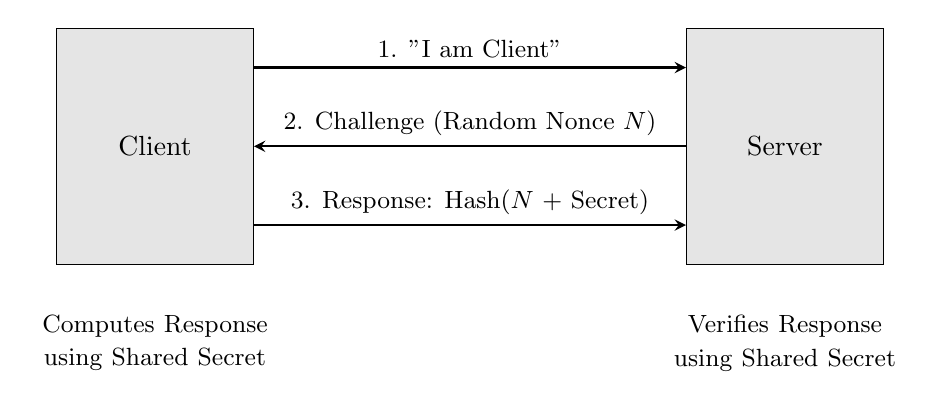
\begin{tikzpicture}[node distance=2cm, auto, >=stealth]
        % Nodes
        \node (client) [draw, rectangle, minimum height=3cm, minimum width=2.5cm, fill=gray!20] {Client};
        \node (server) [draw, rectangle, minimum height=3cm, minimum width=2.5cm, fill=gray!20, right of=client, node distance=8cm] {Server};
        
        % Arrows and text
        \draw[->, thick] ([yshift=1cm]client.east) -- node[above] {\small 1. "I am Client"} ([yshift=1cm]server.west);
        
        \draw[<-, thick] ([yshift=0cm]client.east) -- node[above] {\small 2. Challenge (Random Nonce $N$)} ([yshift=0cm]server.west);
        
        \draw[->, thick] ([yshift=-1cm]client.east) -- node[above] {\small 3. Response: Hash($N$ + Secret)} ([yshift=-1cm]server.west);
        
        % Annotations
        \node at (0, -2.5) [text width=3cm, align=center] {\small Computes Response\\ using Shared Secret};
        \node at (8, -2.5) [text width=3cm, align=center] {\small Verifies Response\\ using Shared Secret};
    \end{tikzpicture}
    \caption{A simple Challenge-Response authentication scheme. Replay attacks are mitigated because the nonce $N$ changes every session.}
    \label{fig:challenge_response}
\end{figure}

In a typical challenge-response scheme (Figure~\ref{fig:challenge_response}), the server sends a random challenge (e.g., a nonce) to the client. The client computes a cryptographic hash of the challenge combined with their secret password and sends it back. The server performs the same computation and verifies the result. Because the challenge changes every time, an attacker eavesdropping on the network cannot reuse the captured hash (\textbf{replay attack}).

\subsection{Secure Password Storage}
Operating systems and web servers must store user credentials. If an attacker compromises the server, the confidentiality of the password file is at risk. 
To minimize this risk:
\begin{itemize}
    \item \textbf{Never store passwords in cleartext.} Passwords must be protected cryptographically using one-way cryptographic hash functions.
    \item \textbf{Use Salting.} A random salt should be added to the password before hashing to defend against precomputed dictionary attacks (Rainbow Tables).
    \item Implement strict access control policies on the password file.
    \item Never disclose the actual secret in password-recovery schemes (e.g., sending the plaintext password via email is a severe security flaw).
\end{itemize}

\begin{tcolorbox}[colback=blue!5!white,colframe=blue!75!black,title=Exam Insight]
A typical exam scenario requires critically analyzing custom password recovery mechanisms. You must check if secrets are transmitted in plaintext, sent over unencrypted channels, or poorly stored in the backend database. You are expected to clearly highlight these vulnerabilities and propose concrete secure storage methods (such as salted hashes using strong one-way functions) and robust exchange protocols (like challenge-response or mutual authentication) as viable countermeasures to reduce the risk.
\end{tcolorbox}

\section{The ``To Have'' Factor: Tokens and Smart Cards}
Here, the user proves they possess a specific physical item.

\subsection{Advantages and Disadvantages}
\textbf{Advantages:} It leverages the human factor, as people are generally more protective of physical items (like keys or phones) than abstract passwords and will quickly notice if they are missing. It offers a good level of security at a relatively low cost.

\textbf{Disadvantages:} Physical tokens are harder to deploy logistically and can be lost or stolen. The primary countermeasure is to use them in combination with a second factor (e.g., a smart card that also requires a PIN).

\subsection{Classic and Modern Technologies}
\begin{itemize}
    \item \textbf{Static OTP Lists:} A cheap alternative where the user and host share a printed list of one-time passwords (e.g., a grid card).
    \item \textbf{Hardware One-Time Password (OTP) Generators:} A device holding a secret key synchronized with the host (via a counter or time). It generates a MAC (Message Authentication Code) that changes every 30-60 seconds.
    \item \textbf{Smart Cards:} Cards equipped with a CPU and non-volatile RAM holding a private key. They authenticate to the host via a challenge-response protocol (signing the challenge). The private key never leaves the tamper-proof device.
    \item \textbf{Modern TOTP Apps:} Software implementations of OTP generators (e.g., Google Authenticator). Unlike hardware tokens, these run on general-purpose smartphones, which introduces the risk of malware compromising the generated codes.
    \item \textbf{Secure Keys (e.g., YubiKeys):} Hardware-based devices that plug into a USB port or use NFC. They provide OTPs or use Public Key Cryptography (FIDO2/WebAuthn) for secure, phishing-resistant authentication.
\end{itemize}

A notable threat to mobile-based authentication (like SMS OTPs) is \textbf{SIM Swapping}, where an attacker uses social engineering against a telecom operator to port the victim's phone number to a SIM card controlled by the attacker.

\section{The ``To Be'' Factor: Biometrics}
Biometric authentication requires the user to prove they possess specific physical or behavioral characteristics. Examples include fingerprints, face geometry, hand geometry, retina/iris scans, voice analysis, DNA, and typing dynamics.

\subsection{Advantages and Disadvantages}
\textbf{Advantages:} High level of security and robustness. It requires no extra hardware for the user to carry around or remember.

\textbf{Disadvantages:} 
\begin{itemize}
    \item Hard to deploy (requires specialized sensors).
    \item \textbf{Probabilistic matching:} Unlike a password which is strictly right or wrong, biometrics rely on similarity thresholds, leading to \textit{false positives} (accepting an impostor) and \textit{false negatives} (rejecting the legitimate user).
    \item Invasive measurement and privacy sensitivity.
    \item Characteristics can change over time (e.g., due to injury or aging).
    \item Issues for users with physical disabilities.
    \item \textbf{Cloning:} Biometric traits can often be captured and replicated (e.g., lifting a fingerprint from a glass, or using high-resolution photos to fool facial recognition).
\end{itemize}

Because biometric traits cannot be easily changed once compromised (you cannot ``reset'' your fingerprint), systems must employ countermeasures like frequent re-measurement, liveness detection (to ensure a real human is present, not a photograph), and providing secure fallback authentication methods.

\section{Novel Factors and Single Sign-On}

\subsection{The ``Social'' Factor}
Experimental authentication methods involve proving \textit{who you know}. For example, Facebook has experimented with social authentication where a user, upon logging in from an unrecognized device, is asked to identify their friends from a selection of photos.

\subsection{Single Sign-On (SSO)}
To combat the fatigue of managing multiple passwords across countless websites, \textbf{Single Sign-On (SSO)} centralizes authentication. The solution involves one identity, 1-2 authentication factors, and one \textit{trusted host} (Identity Provider).

\begin{figure}[h!]
    \centering
    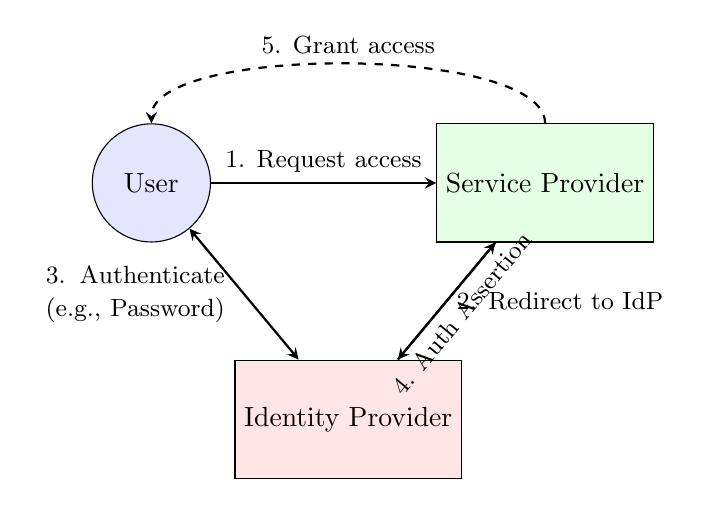
\begin{tikzpicture}[node distance=3cm, auto, >=stealth]
        \node (user) [draw, circle, minimum size=1.5cm, fill=blue!10] {User};
        \node (sp) [draw, rectangle, minimum height=1.5cm, minimum width=2.5cm, fill=green!10, right of=user, node distance=5cm] {Service Provider};
        \node (idp) [draw, rectangle, minimum height=1.5cm, minimum width=2.5cm, fill=red!10, below of=sp, node distance=3cm, xshift=-2.5cm] {Identity Provider};
        
        \draw[->, thick] (user) -- node[above] {\small 1. Request access} (sp);
        \draw[->, thick] (sp) -- node[right] {\small 2. Redirect to IdP} (idp);
        \draw[<->, thick] (user) -- node[left, text width=2.5cm, align=center] {\small 3. Authenticate\\ (e.g., Password)} (idp);
        \draw[->, thick] (idp) -- node[below, sloped] {\small 4. Auth Assertion} (sp);
        \draw[->, thick, dashed] (sp.north) .. controls +(up:1cm) and +(up:1cm) .. node[above] {\small 5. Grant access} (user.north);
    \end{tikzpicture}
    \caption{Simplified Single Sign-On (SSO) flow.}
    \label{fig:sso_flow}
\end{figure}

As shown in Figure~\ref{fig:sso_flow}, the user authenticates once with the trusted host. When accessing other services (Service Providers), those services ask the trusted host to verify the user's identity. Examples include Shibboleth (SAML) used in academia, and OAuth2/OpenID Connect used by major tech companies (e.g., ``Login with Google'').

\textbf{Challenges of SSO:}
\begin{itemize}
    \item It creates a \textbf{single point of trust}. If the identity provider is compromised, all linked services are compromised.
    \item The password reset scheme must be absolutely bulletproof (often relying on email as the root of trust).
    \item The cryptographic flows are complex for developers to implement correctly, often leading to subtle but critical vulnerabilities in the interactions between services.
\end{itemize}

\section{Passwordless Authentication: Passkeys}
The industry is moving toward \textbf{Passwordless Authentication} through the use of \textbf{Passkeys} (built on WebAuthn/FIDO2 standards). 
Instead of a shared secret (password), Passkeys use \textbf{Public Key Cryptography}. 
\begin{enumerate}
    \item \textbf{Registration:} The user's device generates a cryptographic key pair. The \textit{public key} is sent to the application's server. The \textit{private key} is securely stored on the user's device (e.g., in a secure enclave).
    \item \textbf{Login:} The server sends a cryptographic challenge. The user unlocks their private key locally using biometrics (FaceID, TouchID) or a device PIN. The device uses the private key to sign the challenge and returns it to the server, which verifies the signature using the stored public key.
\end{enumerate}
Because the private key never leaves the device, Passkeys are immune to phishing, server data breaches (the server only holds public keys), and credential stuffing attacks.

\section{Conclusions}
Identification, authentication, and authorization are distinct but inter-dependent concepts. There are three main types of authentication factors (to know, to have, to be), and for robust security, they should be used in combination (Multi-Factor Authentication). As traditional passwords increasingly show their limits and vulnerabilities, modern solutions like Password Managers, Single Sign-On, and particularly Passwordless schemes (Passkeys) are paving the way for a more secure and usable future, though they must be implemented and managed with care.

\section*{Chapter Summary}
This chapter explores the foundational concepts and mechanisms of authentication. It distinguishes authentication from identification, and details the Three Factors of Authentication: \textit{To Know} (passwords), \textit{To Have} (tokens), and \textit{To Be} (biometrics). The chapter also covers secure password handling, Single Sign-On (SSO), and modern Passwordless Authentication (Passkeys).

\begin{table}[h!]
    \centering
    \renewcommand{\arraystretch}{1.2}
    \begin{tabular}{|l|p{3.5cm}|p{4.2cm}|p{4.2cm}|}
        \hline
        \textbf{Factor} & \textbf{Examples} & \textbf{Advantages} & \textbf{Disadvantages} \\ \hline
        \textbf{To Know} & Passwords, PINs & Cheap, easy to deploy & Vulnerable to guessing/stealing, hard to remember \\ \hline
        \textbf{To Have} & Smart cards, OTP tokens, YubiKeys & Leverages human protection of physical items & Hard to deploy logistically, can be lost or stolen \\ \hline
        \textbf{To Be} & Fingerprints, Face geometry & High security, robust, no extra hardware & Probabilistic matching, privacy issues, cloning risk \\ \hline
    \end{tabular}
    \caption{Summary of the Three Authentication Factors}
    \label{tab:auth_factors}
\end{table}


% Chapter 4: Access Control
\chapter{Access Control}
\label{ch:access_control}

\section{Introduction to Access Control}
Access control is fundamentally a binary decision mechanism: whenever an entity requests access to a resource, the system must determine whether the action is \textit{allowed} or \textit{denied}. While this concept appears simple on the surface, scaling this binary decision across thousands of users and millions of resources in a modern computing environment is profoundly complex. Administrators cannot explicitly list the answers for every possible access request; instead, they must distill these permissions into robust and generalized \textit{rules}.

The study of access control revolves around three primary questions:
\begin{enumerate}
    \item How do we \textit{design} the access rules?
    \item How do we \textit{express} the access rules in practice?
    \item How do we appropriately \textit{apply} them?
\end{enumerate}

\subsection{Authentication and Authorization}
Before access control can take place, the system must establish identities and evaluate policies. This process is split into two phases:
\begin{itemize}
    \item \textbf{Identification and Authentication:} Verifies the identity of the \textit{principal} (the active entity, such as a human user) making the request, mapping them to a corresponding system \textit{subject} (such as a running process).
    \item \textbf{Authorization:} The process where the system evaluates the subject's request to perform an \textit{access operation} on a passive \textit{object} (such as a file or a network socket), checking against established access control policies.
\end{itemize}

While centralized systems handle this cleanly, distributed systems introduce severe complexities regarding how to discover all relevant policies across nodes, and how to safely make decisions when policies may be missing or unreachable.

\section{The Reference Monitor}
The core component responsible for enforcing access control policies within an operating system is known as the \textbf{Reference Monitor}. It is an abstract machine that mediates all access to objects by subjects, answering the question: ``Who does what on which resource?'' All modern operating system kernels implement some form of a reference monitor.

According to the foundational Anderson report (1972), a Reference Monitor must satisfy three stringent requirements:
\begin{enumerate}
    \item \textbf{Tamper-proof:} It must be impossible for malicious subjects to modify or disable the reference monitor's code or its access control policies.
    \item \textbf{Non-bypassable:} Every single request for resource access must pass through the reference monitor. There can be no alternative paths to the resource.
    \item \textbf{Small enough to be verified:} The implementation must be sufficiently compact and simple so that it can be rigorously tested and mathematically or empirically verified to be correct.
\end{enumerate}

\begin{figure}[htpb]
    \centering
    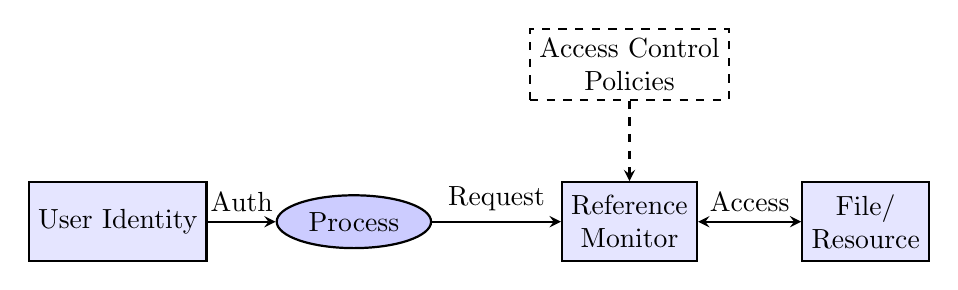
\begin{tikzpicture}[node distance=2.5cm, auto, thick, >=stealth]
        \node[draw, rectangle, fill=blue!10, minimum height=1cm] (principal) {User Identity};
        \node[draw, ellipse, fill=blue!20, right of=principal, node distance=3cm] (subject) {Process};
        \node[draw, rectangle, fill=blue!10, right of=subject, node distance=3.5cm, minimum height=1cm, align=center] (monitor) {Reference\\Monitor};
        \node[draw, rectangle, fill=blue!10, right of=monitor, node distance=3cm, minimum height=1cm, align=center] (object) {File/\\Resource};
        \node[draw, rectangle, dashed, above of=monitor, node distance=2cm, align=center] (policy) {Access Control\\Policies};
        
        \draw[->] (principal) -- node[above] {Auth} (subject);
        \draw[->] (subject) -- node[above] {Request} (monitor);
        \draw[<->] (monitor) -- node[above] {Access} (object);
        \draw[->, dashed] (policy) -- (monitor);
    \end{tikzpicture}
    \caption{The relationship between Principals, Subjects, the Reference Monitor, and Objects.}
    \label{fig:ref_monitor}
\end{figure}

\section{Access Control Models}
Access control models provide the formal framework for how privileges are assigned and evaluated. They can be broadly categorized into three types based on \textit{who} assigns the privileges and how they are structured:
\begin{itemize}
    \item \textbf{Discretionary Access Control (DAC):} The resource owner discretionarily decides who can access their resources.
    \item \textbf{Mandatory Access Control (MAC):} Privileges are strictly set by a central security administrator according to system-wide policies; users cannot override these.
    \item \textbf{Role-Based Access Control (RBAC):} Access is granted based on abstract organizational \textit{roles} rather than raw individual identities.
\end{itemize}
The fundamental difference between DAC and MAC lies precisely in who holds the authority to grant or revoke privileges.

\section{Discretionary Access Control (DAC)}
In a DAC system, the creator or owner of a resource acts as the ultimate authority over it. For example, if Stefano creates a file, he can discretionarily grant Federico the privilege to read it. 

Because this reflects intuitive human ownership, virtually all off-the-shelf operating systems (Windows, Linux, macOS) and applications (like social networks) implement DAC as their primary mechanism.

\subsection{The General Model of DAC (HRU Model)}
To rigorously analyze DAC, we rely on formal models such as the Harrison-Ruzzo-Ullman (HRU) model (derived from Lampson's access matrix). The model identifies three main entities:
\begin{itemize}
    \item \textbf{Subjects ($S$):} Active entities capable of exercising privileges.
    \item \textbf{Objects ($O$):} Passive resources upon which privileges are exercised.
    \item \textbf{Actions ($A$):} Operations that can be performed (e.g., read, write, execute).
\end{itemize}

The \textbf{Protection State} of the system is represented as a triple $(S, O, A)$. The privileges are recorded in an \textbf{Access Control Matrix} $\mathcal{A}$, where $\mathcal{A}[s,o]$ contains the subset of actions $A$ that subject $s$ is authorized to execute on object $o$. 

\subsection{Transitions and Safety Problems}
A system's protection state does not remain static; it undergoes \textit{transitions} via sequences of basic operations. Basic operations include creating or destroying subjects and objects, and adding or removing permissions from the matrix $\mathcal{A}[s,o]$. 

However, transitions must be carefully controlled. A command like ``create file $f$ for user $u$'' must include conditional statements (e.g., checking if $f$ already exists) to prevent hostile takeovers of existing objects.

This dynamicity introduces the \textbf{Safety Problem}: Given an initial configuration and a defined set of transitions, is there any sequence of commands that allows a subject $s$ to obtain a specific right $r$ on an object $f$ without the owner explicitly intending to grant it? If such an unintended leak is possible, the system's commands are \textit{unsafe by design}.

Formally, Harrison, Ruzzo, and Ullman proved that in a generic HRU model with infinite resources, the safety problem is \textbf{undecidable}. It is only mathematically decidable in highly constrained, practically useless environments (such as mono-operational systems) or strictly finite resource bounds.

\subsection{Common Implementations of DAC}
A pure access control matrix is inherently sparse, making it highly inefficient to store directly in memory. Operating systems use alternative data structures:
\begin{itemize}
    \item \textbf{Authorizations Table:} A database table recording only non-null $(S, O, A)$ triples. Commonly used in relational Database Management Systems (DBMS).
    \item \textbf{Access Control Lists (ACLs):} Represents the matrix by \textit{columns}. Each object holds a list of subjects and their permitted actions. This allows highly efficient per-object operations (e.g., ``Who can read this file?'') and is the most common OS implementation.
    \item \textbf{Capability Lists:} Represents the matrix by \textit{rows}. Each subject holds an unforgeable list of objects it can access and the corresponding authorizations (like a ring of keys). It is highly efficient for per-subject operations but suffers because subjects tend to persist while objects are frequently created and destroyed, making revocation difficult.
\end{itemize}

In standard UNIX systems, permissions are further abbreviated into ``triads''. An object specifies privileges for its \textit{User} (owner), \textit{Group}, and \textit{Other} entities, defining Read, Write, and Execute (rwx) rights for each class.

\subsection{Shortcomings of DAC and the Trojan Horse}
Despite its ubiquity, DAC has critical flaws:
\begin{itemize}
    \item As proven by HRU, global safety cannot be guaranteed.
    \item It suffers from poor scalability and management overhead; a single careless user can inadvertently compromise the entire system by exposing sensitive files.
    \item DAC controls access to \textit{objects}, but cannot control the flow of \textit{data} once it is inside a valid subject's memory. This leads to the malicious user and \textbf{Trojan Horse} vulnerabilities.
\end{itemize}

\begin{figure}[htpb]
    \centering
    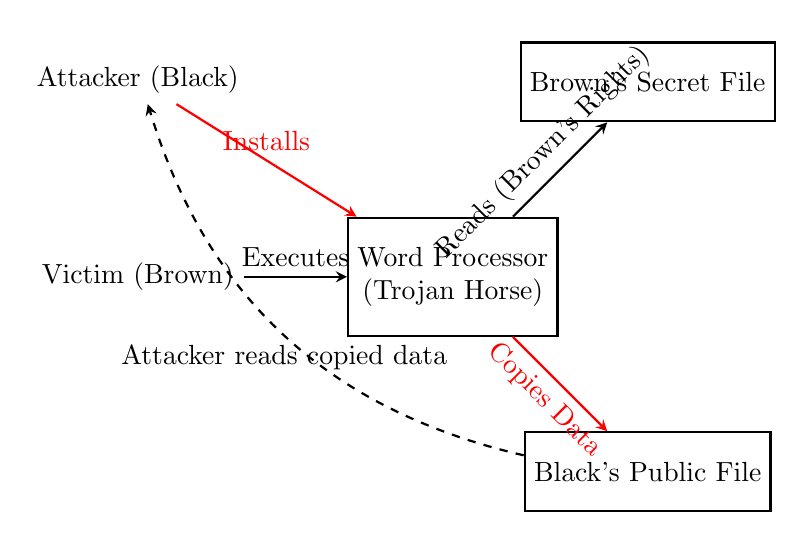
\begin{tikzpicture}[node distance=2.5cm, auto, thick, >=stealth]
        \node (attacker) {Attacker (Black)};
        \node[below of=attacker, node distance=2.5cm] (victim) {Victim (Brown)};
        \node[draw, rectangle, right of=victim, node distance=4cm, minimum height=1.5cm, align=center] (trojan) {Word Processor\\(Trojan Horse)};
        \node[draw, rectangle, above right of=trojan, node distance=3.5cm, minimum height=1cm] (secret) {Brown's Secret File};
        \node[draw, rectangle, below right of=trojan, node distance=3.5cm, minimum height=1cm] (shared) {Black's Public File};

        \draw[->, red] (attacker) -- node[above] {Installs} (trojan);
        \draw[->] (victim) -- node[above] {Executes} (trojan);
        \draw[->] (trojan) -- node[above, sloped] {Reads (Brown's Rights)} (secret);
        \draw[->, red] (trojan) -- node[below, sloped] {Copies Data} (shared);
        \draw[->, dashed, bend left] (shared) to node[below] {Attacker reads copied data} (attacker);
    \end{tikzpicture}
    \caption{The DAC Trojan Horse Problem. The Trojan inherits the victim's privileges to read a secret file, but abuses those privileges to copy the data into an object accessible to the attacker.}
    \label{fig:trojan_horse}
\end{figure}

In a Trojan Horse attack, a victim runs a malicious program. Because DAC grants the running process the same privileges as the victim, the process can legitimately read the victim's secret files. However, the program then maliciously writes that data into a different file owned by the attacker. DAC fails to stop this because the write operation is legitimately authorized under the victim's privileges.

\section{Mandatory Access Control (MAC)}
To solve the catastrophic data leakage inherent in DAC, high-security environments (such as military and intelligence agencies) employ \textbf{Mandatory Access Control (MAC)}. Under MAC, resource owners \textit{cannot} assign privileges. Instead, privileges are deterministically evaluated against system-wide policies defined by a security administrator. Popular MAC implementations include SELinux and AppArmor.

\subsection{Secrecy Levels and Labels}
MAC relies on the concept of \textit{clearance} for subjects and \textit{sensitivity} for objects. These classifications are composed of two parts:
\begin{enumerate}
    \item \textbf{A strictly ordered set of secrecy levels:} Hierarchical tiers of trust. For example, the US government utilizes: \texttt{Top Secret > Secret > FOUO > Unclassified}. NATO utilizes: \texttt{COSMIC Top Secret > NATO Secret > NATO Confidential > Unclassified}.
    \item \textbf{A set of non-hierarchical labels (compartments):} Subject-matter categories, such as \texttt{Nuclear, Crypto, Finance, Policy}.
\end{enumerate}

When combined, these elements form \textbf{Lattice-Based Access Control (LBAC)}. A classification is a pair $C = \{Level, Labels\}$. The relationships form a partial order (a mathematical lattice) defined by dominance:
\[ \{C_1, L_1\} \ge \{C_2, L_2\} \iff C_1 \ge C_2 \text{ and } L_2 \subseteq L_1 \]

A subject only dominates an object if the subject's hierarchical level is greater than or equal to the object's, \textit{and} the subject possesses all the specific compartment labels assigned to the object.

\subsection{The Bell-LaPadula Model (BLP)}
The most famous formalization of MAC for preserving confidentiality is the Bell-LaPadula (BLP) model. It overlays MAC rules on top of standard DAC. It relies on two fundamental MAC properties to prevent data leakage:
\begin{enumerate}
    \item \textbf{Rule 1 - The Simple Security Property (No Read Up):} A subject at a given secrecy level cannot read an object at a higher secrecy level.
    \item \textbf{Rule 2 - The Star Property ($\star$-property) (No Write Down):} A subject at a given secrecy level cannot write to an object at a lower secrecy level.
\end{enumerate}
Additionally, BLP defines \textbf{Rule 3 (Discretionary Security Property)}, requiring that any access must also be permitted by the underlying DAC access matrix.

The $\star$-property elegantly neutralizes the Trojan Horse problem. If a victim executes a Trojan, the process runs at the victim's high clearance level. The process can read the victim's high-secret files, but when the Trojan attempts to copy the data to the attacker's low-clearance file, the operation is rejected as an illegal ``write down.''

\subsubsection{Tranquility and Monotonic Flow}
The BLP model relies on the \textbf{Tranquility Property}, dictating that the security levels of active subjects and objects cannot change dynamically during execution. 

Because subjects can read down and write up, BLP creates a \textit{monotonic flow of information} toward higher secrecy levels. Data acts like a gas floating upwards; it can never organically descend to a lower classification. Consequently, BLP systems require highly \textit{trusted subjects}—special administrative processes exempt from the $\star$-property—to declassify or sanitize documents and move them down the lattice.

It is critical to note that BLP is designed exclusively for confidentiality. It \textit{does not address integrity} (preventing unauthorized modification of high-level data by low-level subjects). To secure integrity, systems often run a parallel model, such as the \textbf{Biba Model}, which limits modifications based on data trust levels.

\section{Conclusion}
Access control bridges the gap between verified authentication and safe resource utilization. Discretionary Access Control (DAC) provides the highly flexible, intuitive owner-centric model that dominates consumer and commercial software. However, due to its vulnerability to information leakage and Trojan attacks, strict environments layer Mandatory Access Control (MAC) atop DAC, utilizing mathematical models like Bell-LaPadula to forcefully dictate the flow of sensitive information.


% Chapter 5: Introduction to Software Security
\chapter{Introduction to Software Security}

\section{Fundamentals of Software Security}
\subsection{Software Requirements and Security}
Good software engineering aims to meet a specific set of requirements, which can be broadly divided into functional and non-functional categories. 
\begin{itemize}
    \item \textbf{Functional requirements} specify what the software must do. They define the intended behavior and the tasks the software is designed to accomplish.
    \item \textbf{Non-functional requirements} specify how the software should perform its tasks. These include usability, performance, reliability, safety, and, crucially, \textbf{security}.
\end{itemize}

Creating inherently secure applications is a fundamental, yet often unknown, skill for a good developer or software engineer. Creating secure software is inherently difficult because security is a negative goal: it is about preventing unwanted behaviors rather than just ensuring desired ones. 

\subsection{Bugs, Vulnerabilities, and Exploits}

\begin{tcolorbox}[colback=blue!5!white,colframe=blue!75!black,title=Exam Insight]
Questions about this topic are usually based on identifying assets at risk, associated threats, threat agents, and assessing vulnerabilities for a given scenario (e.g., floor cleaning robots, tracking devices, infrastructure). You may be asked to analyze vulnerabilities, explain potential exploits, and propose concrete countermeasures to reduce risk. Furthermore, be prepared to suggest potential attack surfaces for a described infrastructure, analyze custom authentication mechanisms to highlight weaknesses (like snooping or guessing), and correct Risk Analysis Tables (Likelihood/Impact) while justifying your changes and selecting the best countermeasures.
\end{tcolorbox}

Software is designed to implement specifications. When these specifications are not met, the software contains flaws.
\begin{itemize}
    \item An unmet functional specification results in a \textbf{software bug}.
    \item An unmet security specification results in a \textbf{vulnerability}.
\end{itemize}

It is important to distinguish between a vulnerability and an exploit. A vulnerability is a weakness in the system, whereas an \textbf{exploit} is a specific method, piece of code, or technique used to leverage a vulnerability to violate a system's security properties (Confidentiality, Integrity, Availability - CIA). 
Therefore, having a vulnerability does not necessarily mean an exploit exists, although it opens the door for one to be developed.

\section{The Vulnerability Lifecycle and Disclosure}

\subsection{The Lifecycle of a Vulnerability}
The life of a software vulnerability can be represented as a timeline of key events, from its introduction into the codebase to its eventual remediation. 

\begin{figure}[hbtp]
\centering
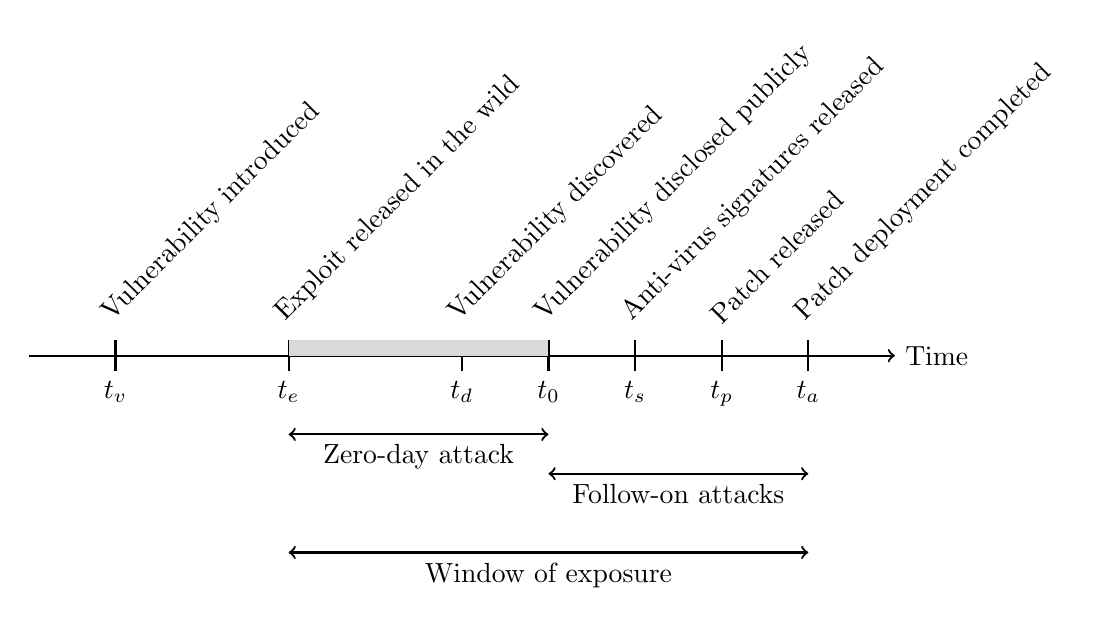
\begin{tikzpicture}[xscale=1.1, yscale=1]
\draw[->, thick] (0,0) -- (10,0) node[right] {Time};

\draw[thick] (1,-0.2) node[below] {$t_v$} -- (1,0.2) node[above, rotate=45, anchor=south west] {Vulnerability introduced};
\draw[thick] (3,-0.2) node[below] {$t_e$} -- (3,0.2) node[above, rotate=45, anchor=south west] {Exploit released in the wild};
\draw[thick] (5,-0.2) node[below] {$t_d$} -- (5,0.2) node[above, rotate=45, anchor=south west] {Vulnerability discovered};
\draw[thick] (6,-0.2) node[below] {$t_0$} -- (6,0.2) node[above, rotate=45, anchor=south west] {Vulnerability disclosed publicly};
\draw[thick] (7,-0.2) node[below] {$t_s$} -- (7,0.2) node[above, rotate=45, anchor=south west] {Anti-virus signatures released};
\draw[thick] (8,-0.2) node[below] {$t_p$} -- (8,0.2) node[above, rotate=45, anchor=south west] {Patch released};
\draw[thick] (9,-0.2) node[below] {$t_a$} -- (9,0.2) node[above, rotate=45, anchor=south west] {Patch deployment completed};

\draw[<->, thick] (3,-1) -- (6,-1) node[midway, below] {Zero-day attack};
\draw[<->, thick] (6,-1.5) -- (9,-1.5) node[midway, below] {Follow-on attacks};
\draw[<->, thick] (3,-2.5) -- (9,-2.5) node[midway, below] {Window of exposure};

\fill[gray!30] (3,0) rectangle (6,0.2);
\end{tikzpicture}
\caption{The Vulnerability Lifecycle, illustrating the timeline of disclosure and patching.}
\end{figure}

The period between the exploit release ($t_e$) and public disclosure ($t_0$) is particularly dangerous; attacks occurring during this time are known as \textbf{Zero-day attacks}. The overall \textbf{window of exposure} lasts until the patch is widely deployed ($t_a$).

\subsection{Disclosure Policies}
The history of software vulnerabilities is heavily influenced by how they are disclosed to the public. The debate over disclosure policies has evolved over the years:
\begin{itemize}
    \item \textbf{Non-Disclosure:} Keeping the vulnerability secret to prevent exploitation. However, this often leaves users unprotected if malicious actors find the vulnerability independently.
    \item \textbf{Full Disclosure:} Publishing all details of the vulnerability immediately, forcing vendors to patch quickly but also arming attackers with exploit details.
    \item \textbf{Coordinated Disclosure (or Anti-Disclosure in its extreme):} Working with the vendor to release a patch simultaneously with the vulnerability details, minimizing the zero-day window.
\end{itemize}

\subsection{The Economics of Vulnerabilities: Black Markets and Bug Bounties}
With the rise of the internet, a lucrative \textbf{black market} for exploits emerged. Attackers are willing to pay significant amounts for zero-day exploits. To counter this, legitimate organizations and security platforms (e.g., Bugcrowd, HackerOne) introduced \textbf{Bug Bounties}. These programs financially reward security researchers for responsibly disclosing vulnerabilities, providing an economic incentive to report bugs rather than sell them to malicious actors.

\section{Permissions and Privilege Escalation in UNIX}

\subsection{UNIX Process Privileges: RUID, EUID, and SUID}
To understand software vulnerabilities in practice, we examine process privileges in UNIX-like operating systems. In UNIX, every file has an owner. For example, a file might be owned by user \texttt{foo}.

When a user (e.g., \texttt{bar}) executes a program, the resulting process runs with certain user IDs:
\begin{itemize}
    \item \textbf{Real UID (RUID):} Represents the real owner of the process (the user who executed it, i.e., \texttt{bar}).
    \item \textbf{Effective UID (EUID):} The UID used by the operating system for checking access permissions. Normally, the EUID is equal to the RUID.
    \item \textbf{Saved set-user-ID (SUID):} A special permission bit that can be set on an executable file. If an executable has the SUID bit set, the EUID of the process running it is changed to the owner of the file, rather than the user who executed it.
\end{itemize}

For example, if an executable owned by \texttt{root} has the SUID bit set (\texttt{rwsr-xr-x}), and user \texttt{bar} executes it, the process will have an RUID of \texttt{bar} but an EUID of \texttt{root}. This allows the program to perform privileged operations on behalf of the unprivileged user.

\begin{figure}[hbtp]
\centering
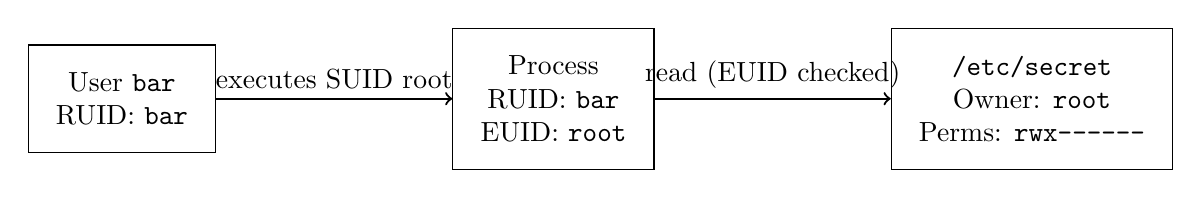
\begin{tikzpicture}
\node[draw, rectangle, inner sep=10pt, align=center] (user) {User \texttt{bar}\\RUID: \texttt{bar}};
\node[draw, rectangle, inner sep=10pt, align=center, right=3cm of user] (proc) {Process\\RUID: \texttt{bar}\\EUID: \texttt{root}};
\node[draw, rectangle, inner sep=10pt, align=center, right=3cm of proc] (file) {\texttt{/etc/secret}\\Owner: \texttt{root}\\Perms: \texttt{rwx------}};

\draw[->, thick] (user) -- node[above] {executes SUID root} (proc);
\draw[->, thick] (proc) -- node[above] {read (EUID checked)} (file);
\end{tikzpicture}
\caption{The SUID mechanism allowing an unprivileged user to execute a process with elevated permissions.}
\end{figure}

\subsection{A Practical Vulnerability Example}
Consider a program designed to read a sensitive file (\texttt{/etc/secret}) accessible only by \texttt{root}, process the configuration, and perform some actions. Because it needs to read a root-owned file, the program is compiled and set with the SUID root bit.

\begin{verbatim}
#include <unistd.h>
#include <stdio.h>

int main(int argc, const char *argv[]) {
    FILE *fp;
    char line[1024];
    
    // The process has EUID = root because of the SUID bit
    fp = fopen("/etc/secret", "r"); 
    
    while (!feof(fp)) {
        fgets(line, 1024, fp);
        puts(line);
    }
    fclose(fp);
    return 0;
}
\end{verbatim}

If this program simply reads \texttt{/etc/secret} and prints it, any user executing this SUID binary can read the secret file. If the program was intended to only parse the file and return an "OK" status but instead prints the file contents on a parsing error, an attacker could craft a malicious input or exploit a parsing bug to force the program to reveal the secret file or execute arbitrary code while retaining \texttt{root} privileges.

\subsection{Exploitation and Patching}

\begin{tcolorbox}[colback=blue!5!white,colframe=blue!75!black,title=Exam Insight]
Exam questions often ask you to identify vulnerabilities in C source code (specifically focusing on Buffer Overflows or Format Strings), find the vulnerable lines, explain whether they are exploitable, and propose fixes (such as dropping privileges appropriately or sanitizing inputs). You may also need to describe the steps and assumptions required to write exploits, draw memory stack layouts before and after execution, and analyze the bypass or effect of mitigations like NX, ASLR, or Stack Canaries.
\end{tcolorbox}

The core issue is that the program holds elevated privileges (EUID = \texttt{root}) for longer than necessary, expanding the \textbf{attack surface}. Any bug in the \texttt{parse()} function or subsequent logic can be exploited with root privileges.

To patch this, developers must apply the principle of privilege separation:
\begin{enumerate}
    \item Acquire privileges only when absolutely necessary.
    \item Perform the privileged operation (e.g., opening the file).
    \item \textbf{Drop the privileges definitively} immediately after the operation is complete.
\end{enumerate}

\begin{verbatim}
    // ...
    fp = fopen("/etc/secret", "r");
    
    // Drop privileges: set EUID back to RUID
    setuid(getuid()); 
    
    // Now execute parsing and unprivileged logic
    fgets(line, 1024, fp);
    // ...
\end{verbatim}
By dropping the privileges before parsing the file, even if the parsing logic contains a vulnerability (like a buffer overflow), the exploit will only execute with the unprivileged user's permissions, severely limiting the impact.

\section{Principles of Secure Design}

\subsection{Core Principles}
Designing secure software requires adherence to several fundamental principles:
\begin{itemize}
    \item \textbf{Reduce privileged parts to a minimum:} Minimize the amount of code that runs with elevated privileges.
    \item \textbf{KISS (Keep It Simple, Stupid):} Complexity is the enemy of security. Simple code is easier to audit, test, and secure.
    \item \textbf{Discard privileges definitively:} As shown in the UNIX example, drop elevated privileges (e.g., reverting EUID to RUID) as soon as they are no longer needed.
    \item \textbf{Open design:} Following Kerckhoffs's principle, the security of a system should not rely on the obscurity of its design or implementation. Security through obscurity is not true security.
    \item \textbf{Fail-safe and default deny:} Systems should fail securely. By default, access should be denied, and explicit permission must be granted.
\end{itemize}

\subsection{Secure Development Practices}
In addition to core principles, specific practices should be integrated into the development lifecycle:
\begin{itemize}
    \item \textbf{Handle concurrency carefully:} Concurrency and race conditions (like Time-of-Check to Time-of-Use, TOCTOU) are notoriously tricky to secure and often lead to vulnerabilities.
    \item \textbf{Avoid risky resources:} Do not use unsafe shared resources (like \texttt{mktemp} in shared directories) or unknown, untrusted third-party libraries.
    \item \textbf{Filter input and output:} Never trust user input. Validate, sanitize, and filter all data entering and leaving the system.
    \item \textbf{Use trusted cryptography:} Do not write your own cryptographic primitives, password hashing, or secret management code. Use well-established, audited libraries.
    \item \textbf{Use trustworthy Random Number Generators (RNGs):} Rely on secure sources of randomness, such as \texttt{/dev/urandom} or \texttt{/dev/random} in UNIX-like systems.
\end{itemize}

\section{Conclusion and Future Topics}
In conclusion, it is crucial to recognize that \textbf{bug-free software does not exist}, and achieving vulnerability-free software is exceedingly difficult. Not all bugs lead to vulnerabilities, and not all vulnerabilities currently have working exploits, but the risk remains.

In subsequent chapters, we will explore specific examples of insecure programming in depth:
\begin{itemize}
    \item \textbf{Memory errors in desktop applications:} Buffer overflow bugs and format string bugs.
    \item \textbf{Code-injection bugs in web applications:} SQL injection (SQLi), Cross-Site Scripting (XSS), and Cross-Site Request Forgery (CSRF).
\end{itemize}

\section*{Chapter Summary}
This chapter introduces the fundamental concepts of software security, distinguishing between bugs, vulnerabilities, and exploits. It covers the vulnerability lifecycle, disclosure policies, and the economics of exploits. It also examines UNIX process privileges (RUID, EUID, SUID) as a practical example of vulnerabilities, highlighting privilege separation and dropping. Finally, it outlines core principles of secure design and development practices.

\begin{table}[hbtp]
\centering
\begin{tabular}{|l|p{10cm}|}
\hline
\textbf{Concept} & \textbf{Description} \\
\hline
\textbf{Software Bug} & An unmet functional specification. \\
\hline
\textbf{Vulnerability} & An unmet security specification (a weakness in the system). \\
\hline
\textbf{Exploit} & A method or code used to leverage a vulnerability to violate security properties. \\
\hline
\textbf{Zero-day Attack} & An attack that occurs between the release of an exploit and the deployment of a patch. \\
\hline
\textbf{SUID (UNIX)} & A permission bit that changes the Effective UID of a process to the file owner's UID. \\
\hline
\textbf{Secure Design} & Core principles like keeping it simple, minimizing privileges, failing securely, and open design. \\
\hline
\end{tabular}
\caption{Key Software Security Concepts}
\end{table}


% Chapter 6: Buffer Overflows
\chapter{Buffer Overflows}



\section{Introduction to Buffer Overflows}
A buffer overflow is a classic and prevalent software vulnerability that occurs when a program writes more data to a block of memory, or buffer, than it was allocated to hold. Because buffers are created to contain a specific amount of data, the extra data overwrites adjacent memory locations. In languages like C and C++, which do not inherently perform bounds checking on array and pointer operations, it is left to the developer to ensure that data written to a buffer does not exceed its capacity.

When a buffer overflow occurs on the call stack, it can corrupt data that is critical to the program's control flow, such as the saved return address or the saved base pointer. By carefully crafting the input that causes the overflow, an attacker can overwrite these control values to redirect the program's execution flow to arbitrary code of their choosing, often referred to as shellcode.

\section{Binary Formats and Execution}
Before delving into the mechanics of buffer overflows, it is essential to understand how high-level code is transformed into machine code and how it is structured within an executable file.

\subsection{From Source to Machine Code}
The process of transforming source code into an executable binary involves several stages:
\begin{enumerate}
    \item \textbf{Compiler}: Translates high-level source code (e.g., C) into assembly language, specific to the target architecture.
    \item \textbf{Assembler}: Converts the assembly language instructions into raw machine code (object files).
    \item \textbf{Linker}: Combines one or more object files and libraries into a single executable binary.
\end{enumerate}
Conversely, \textbf{disassemblers} can translate machine code back into assembly, and \textbf{decompilers} attempt to reconstruct the high-level source code from the assembly or machine code.

\subsection{The ELF Binary Format}
On Linux, the standard executable format is the Executable and Linkable Format (ELF). An ELF binary contains information about how the file is organized on disk and how it should be loaded into memory. It contains several key sections:
\begin{itemize}
    \item \textbf{ELF Header}: Describes the high-level structure, file type (executable or library), target machine architecture, and entry point.
    \item \textbf{Program Headers}: Describe how the file will be loaded into memory at runtime, mapping sections into segments.
    \item \textbf{Section Headers}: Describe the binary as it resides on disk, defining sections such as:
    \begin{itemize}
        \item \texttt{.text}: Contains the executable machine instructions of the program.
        \item \texttt{.rodata}: Contains read-only data (e.g., string literals).
        \item \texttt{.data}: Contains initialized global and static variables.
        \item \texttt{.bss}: Contains uninitialized global and static variables (zeroed at runtime).
    \end{itemize}
\end{itemize}

\section{Process Memory Layout in Linux}
When a program is executed, the Linux kernel creates a virtual address space for the process. This virtual memory abstracts the physical memory, giving the process the illusion of having a contiguous, isolated memory space. The dynamic linker and loader map the segments defined in the ELF file into this virtual address space.

For a 32-bit x86 architecture, the typical memory layout of a process from lower to higher addresses is:
\begin{itemize}
    \item \textbf{Text Segment (\texttt{.text})}: Loaded at the bottom (e.g., \texttt{0x08048000}), containing the executable code.
    \item \textbf{Data Segment (\texttt{.data} and \texttt{.bss})}: Placed above the text segment, holding global variables.
    \item \textbf{Heap}: Grows upwards towards higher memory addresses. It is used for dynamically allocated memory (e.g., via \texttt{malloc()}).
    \item \textbf{Memory Mapping Segment}: Used for shared libraries and memory-mapped files.
    \item \textbf{Stack}: Located at the top of the user space (e.g., starting just below \texttt{0xC0000000}) and grows downwards towards lower memory addresses. It stores local variables, function parameters, and control information.
    \item \textbf{Kernel Space}: The topmost portion of the address space (from \texttt{0xC0000000} to \texttt{0xFFFFFFFF}), reserved for the kernel and inaccessible to user-mode code.
\end{itemize}

\section{The Stack and Function Calls}

\begin{tcolorbox}[colback=blue!5!white,colframe=blue!75!black,title=Exam Insight]
Questions on this topic often require you to strictly and clearly draw the process memory stack layout. You must map the stack state right before and after the execution of a vulnerable line or an exploit payload. Be sure to show exactly where local variables, the Stack Pointer (\texttt{ESP}), Base Pointer (\texttt{EBP}), and the saved Return Address (\texttt{EIP}) are located, as this demonstrates a solid understanding of the stack's mechanics.
\end{tcolorbox}

The stack is a Last-In, First-Out (LIFO) data structure fundamental to the execution of functions. It is used to manage function activation records (or stack frames). 

\subsection{Registers}
The x86 architecture relies on several CPU registers to manage the execution state and the stack:
\begin{itemize}
    \item \textbf{General Purpose Registers}: \texttt{EAX}, \texttt{EBX}, \texttt{ECX}, \texttt{EDX} are used for arithmetic operations and data manipulation.
    \item \textbf{Stack Pointer (\texttt{ESP})}: Holds the memory address of the top of the stack. Since the stack grows downwards, pushing a value decrements \texttt{ESP}, and popping a value increments \texttt{ESP}.
    \item \textbf{Base Pointer / Frame Pointer (\texttt{EBP})}: Points to the base of the current function's stack frame. It acts as a stable reference point to access local variables (at negative offsets from \texttt{EBP}) and function arguments (at positive offsets from \texttt{EBP}).
    \item \textbf{Instruction Pointer (\texttt{EIP})}: Holds the address of the next machine instruction to be executed.
\end{itemize}

\subsection{Stack Instructions}
\begin{itemize}
    \item \texttt{push <value>}: Decrements \texttt{ESP} by 4 bytes (on 32-bit) and writes the value to the new address pointed to by \texttt{ESP}.
    \item \texttt{pop <register>}: Reads the value at the address pointed to by \texttt{ESP} into the register, then increments \texttt{ESP} by 4 bytes.
\end{itemize}

\subsection{Function Prologue and Epilogue}
When a function is called, the control flow must jump to the function's code, but it must also remember where to return once the function finishes. The \texttt{call} instruction implicitly pushes the current \texttt{EIP} (the return address) onto the stack before jumping to the target function.

Upon entering the function, the \textbf{Function Prologue} executes to set up the new stack frame:
\begin{verbatim}
push %ebp        ; Save the caller's EBP onto the stack
mov  %esp, %ebp  ; Set the new EBP to the current ESP (top of stack)
sub  $0xX, %esp  ; Allocate space for local variables by decrementing ESP
\end{verbatim}

When the function completes, the \textbf{Function Epilogue} executes to tear down the stack frame and return to the caller:
\begin{verbatim}
leave            ; Equivalent to: mov %ebp, %esp ; pop %ebp
ret              ; Pops the saved return address into EIP and jumps to it
\end{verbatim}

\section{Buffer Overflow Vulnerabilities}

\begin{tcolorbox}[colback=blue!5!white,colframe=blue!75!black,title=Exam Insight]
You will likely be asked to identify binary vulnerabilities (specifically Buffer Overflows and Format String bugs) directly from provided C source code. Be prepared to pinpoint the exact vulnerable lines, explain in detail why they are exploitable based on the provided context, and propose secure coding alternatives or functions (e.g., using \texttt{strncpy} instead of \texttt{strcpy}) to fix the issues.
\end{tcolorbox}

A buffer overflow vulnerability usually stems from the use of unsafe C library functions that copy data into a buffer without verifying if the data fits within the allocated size. Examples of such dangerous functions include \texttt{gets()}, \texttt{strcpy()}, \texttt{strcat()}, \texttt{sprintf()}, and \texttt{scanf()}.

Consider a function \texttt{foo()} that allocates a local 8-byte character array \texttt{char buf[8];} and then calls \texttt{gets(buf);}. The stack frame for \texttt{foo()} will look roughly like this:
\begin{itemize}
    \item Higher Addresses
    \item Function Arguments
    \item Saved \texttt{EIP} (Return Address)
    \item Saved \texttt{EBP}
    \item \texttt{buf[4-7]}
    \item \texttt{buf[0-3]} $\leftarrow$ \texttt{ESP} points near here
    \item Lower Addresses
\end{itemize}

Because \texttt{gets()} does not stop reading until it encounters a newline or EOF, an attacker can provide an input longer than 8 bytes. The data will fill \texttt{buf}, overflow into the saved \texttt{EBP}, and critically, overwrite the saved \texttt{EIP}. When \texttt{foo()} executes the \texttt{ret} instruction, the CPU will pop the attacker's corrupted value into the \texttt{EIP} register and attempt to execute code at that arbitrary address, leading to a crash (Segmentation Fault) or, worse, arbitrary code execution.

\section{Exploitation Techniques}

\begin{tcolorbox}[colback=blue!5!white,colframe=blue!75!black,title=Exam Insight]
A common exam exercise involves practically writing exploits. You should practice describing the necessary steps and underlying assumptions, and then constructing the exact payload required to exploit a Stack-based Buffer Overflow or Format String vulnerability. Often, the goal is to execute injected shellcode or strategically overwrite specific program variables to alter the program's control flow.
\end{tcolorbox}

If an attacker can overwrite the saved \texttt{EIP}, the next step is to point it to a memory location containing valid, malicious machine code, commonly referred to as \textbf{shellcode}.

\subsection{Shellcode}
Historically, the primary goal of an exploit is to spawn a shell (e.g., \texttt{/bin/sh}), granting the attacker command-line access to the victim's machine. The shellcode is the sequence of raw machine instructions that achieves this, typically by invoking the \texttt{execve} system call.

Writing shellcode involves:
\begin{enumerate}
    \item Writing the desired logic in assembly or C.
    \item Ensuring the code is position-independent (it must run regardless of where it is loaded in memory).
    \item Eliminating all null bytes (\texttt{0x00}), as string-handling functions like \texttt{strcpy()} terminate copying upon encountering a null byte, which would truncate the shellcode.
\end{enumerate}

To execute \texttt{execve("/bin/sh", NULL, NULL)}, the shellcode must place the string \texttt{"/bin/sh"} in memory, set up pointers to it, load the system call number (\texttt{0xb} or 11) into \texttt{EAX}, put the address of the string in \texttt{EBX}, set \texttt{ECX} and \texttt{EDX} to NULL, and execute the software interrupt \texttt{int \$0x80} to transition to kernel mode.

A common technique to dynamically find the address of the \texttt{"/bin/sh"} string within the shellcode is the \textbf{Jump and Call Trick}. The shellcode starts with a \texttt{jmp} instruction to a \texttt{call} instruction at the end. The \texttt{call} jumps back to the main payload, pushing the address of the instruction immediately following it onto the stack. By placing the string \texttt{"/bin/sh"} immediately after the \texttt{call}, the payload can simply \texttt{pop} the string's address from the stack into a register.

\subsection{Stack Smashing and NOP Sleds}
If the vulnerable buffer is large enough, the attacker can inject the shellcode directly into it. The payload structure typically consists of:
\[ [\text{NOP Sled}] + [\text{Shellcode}] + [\text{Padding}] + [\text{Target Address for EIP}] \]

The target address overwriting the saved \texttt{EIP} must point precisely to the start of the shellcode. However, predicting the exact address of the buffer in memory can be difficult due to environmental variations. To mitigate this precision problem, attackers use a \textbf{NOP sled}.

A NOP sled is a sequence of \texttt{NOP} (\texttt{0x90} on x86) instructions prepended to the shellcode. A \texttt{NOP} instruction tells the CPU to "do nothing" and move to the next instruction. By filling a large portion of the buffer with a NOP sled, the attacker only needs to guess an address that falls \textit{anywhere} within the sled. The CPU will "slide" down the NOP instructions until it naturally reaches and executes the shellcode.

\subsection{Exploiting via Environment Variables}
When the vulnerable buffer is too small to contain the shellcode, the attacker can place the shellcode in an environment variable. Environment variables are loaded into the process's memory space at high addresses (above the stack).

The attacker creates an environment variable containing a massive NOP sled followed by the shellcode. Then, they provide a small payload to the vulnerable program that simply overflows the buffer enough to overwrite the saved \texttt{EIP} with the estimated address of the environment variable.

\subsection{Advanced Exploitation}
When direct code injection on the stack is prevented by security mechanisms, attackers pivot to alternative strategies:
\begin{itemize}
    \item \textbf{Frame Teleporting}: Instead of overwriting \texttt{EIP}, the attacker overwrites the saved \texttt{EBP}. When the function returns, the caller's stack frame is shifted to a location controlled by the attacker.
    \item \textbf{Return-to-libc (ret2libc)}: Instead of injecting new code, the attacker overwrites the saved \texttt{EIP} with the address of an existing function within the standard C library (libc), such as \texttt{system()}. The attacker also crafts the stack to provide the necessary arguments (like the string \texttt{"/bin/sh"}) to the called function. This is a rudimentary form of Code-Reuse Attacks, which evolved into Return-Oriented Programming (ROP).
\end{itemize}

\section{Defenses Against Buffer Overflows}

\begin{tcolorbox}[colback=blue!5!white,colframe=blue!75!black,title=Exam Insight]
Be prepared to deeply analyze exploit mitigations and discuss how they can be bypassed. Exam questions frequently ask you to explain the effects of specific defenses like NX (Non-Executable Stack), ASLR, or Stack Canaries. Furthermore, you will need to evaluate whether alternative exploitation techniques (such as returning to the \texttt{.text} segment, or leveraging a Format String attack instead of a standard Buffer Overflow) can be used to effectively circumvent these defensive mechanisms.
\end{tcolorbox}

Modern software and operating systems employ a multi-layered defense strategy to mitigate buffer overflow attacks.

\subsection{Source Code Defenses}
The most robust defense is preventing the vulnerability at the source:
\begin{itemize}
    \item \textbf{Safe Libraries}: Replacing unsafe functions with bounded alternatives, such as using \texttt{strncpy()} instead of \texttt{strcpy()}, or using BSD extensions like \texttt{strlcpy()} and \texttt{strlcat()}.
    \item \textbf{Memory-Safe Languages}: Developing in languages that perform automatic bounds checking and dynamic memory management (e.g., Java, Python, Rust) eliminates classical buffer overflows by design.
    \item \textbf{Source Code Analyzers}: Using static analysis tools during the Software Development Life Cycle (SDLC) to automatically detect potential buffer overflows.
\end{itemize}

\subsection{Compiler Level Defenses}
Compilers can instrument the generated code to detect and block overflows at runtime:
\begin{itemize}
    \item \textbf{Stack Canaries (StackGuard)}: The compiler inserts a random "canary" value on the stack between the local variables and the saved control data (\texttt{EBP} and \texttt{EIP}). Before the function returns, the epilogue checks if the canary value has been altered. Since a contiguous buffer overflow must overwrite the canary to reach the saved \texttt{EIP}, the modification is detected, and the program is forcibly aborted. Canaries can be completely random, XORed with the return address, or contain terminator characters (like \texttt{\textbackslash 0}) to stop string-copying functions prematurely.
\end{itemize}

\subsection{Operating System Level Defenses}
Operating systems enforce policies to make exploitation difficult even if a vulnerability exists:
\begin{itemize}
    \item \textbf{Non-Executable Stack (NX Bit / DEP)}: The OS marks the stack and heap memory segments as non-executable (Data Execution Prevention). If an attacker successfully redirects the \texttt{EIP} to their injected shellcode on the stack, the CPU will refuse to execute it and will terminate the process. This forces attackers to rely on complex code-reuse techniques like ROP.
    \item \textbf{Address Space Layout Randomization (ASLR)}: The OS randomly shifts the memory locations of the stack, heap, and libraries every time the program is executed. This randomness makes it extremely difficult for an attacker to reliably predict the target addresses needed to overwrite the \texttt{EIP} or to locate libc functions for a ret2libc attack.
\end{itemize}

\section*{Chapter Summary}

This chapter covers the classic \textbf{Buffer Overflow} vulnerability, explaining how it occurs and how attackers exploit it to gain arbitrary code execution. It details the process memory layout, the call stack, exploitation techniques, and defensive mitigations.

\begin{table}[htpb]
\centering
\begin{tabular}{|l|p{10cm}|}
\hline
\textbf{Concept} & \textbf{Description} \\ \hline
Vulnerability Mechanics & Overwriting bounds via unsafe C functions (e.g., \texttt{strcpy}, \texttt{gets}). \\ \hline
Shellcode & Position-independent machine code injected by attackers. \\ \hline
Exploitation Techniques & Stack Smashing, NOP Sleds, Environment Variables, ret2libc. \\ \hline
Defenses \& Mitigations & Safe libraries, Stack Canaries, NX Bit (DEP), ASLR. \\ \hline
\end{tabular}
\caption{Key concepts in Buffer Overflows.}
\label{tab:ch6_summary}
\end{table}


% Chapter 7: Format String Bugs
\chapter{Format String Bugs}
\label{ch:format_string_bugs}

\begin{tcolorbox}[colback=blue!5!white,colframe=blue!75!black,title=Chapter Summary]
This chapter explores how format string functions like \texttt{printf} can be exploited when user-supplied input is directly passed as the format string. It covers the mechanisms of leaking stack memory, arbitrary memory reads, and arbitrary memory writes, culminating in full execution hijacking using staged writes.

\vspace{2mm}
\begin{center}
\begin{tabular}{|l|p{10cm}|}
\hline
\textbf{Specifier} & \textbf{Exploitation Usage} \\
\hline
\texttt{\%x} & Leaks raw values from the stack sequentially. \\
\texttt{\%N\$x} & Direct parameter access to read the $N$-th parameter on the stack. \\
\texttt{\%s} & Arbitrary read: dereferences a pointer and reads memory until a null byte. \\
\texttt{\%n} & Arbitrary write: writes the number of characters printed so far to a pointer. \\
\texttt{\%hn} & Staged arbitrary write: writes the counter as a 16-bit short integer. \\
\hline
\end{tabular}
\end{center}
\end{tcolorbox}

\section{Introduction to Format Strings}
In C and many other programming languages, printing functions often require a way to embed dynamically evaluated variables into text output. The solution to this problem is the \emph{format string}, a template containing text and special directives known as \emph{placeholders}. These placeholders tell the function how to format the data provided as subsequent arguments.

Common printing functions in C that utilize format strings include \texttt{printf}, \texttt{fprintf}, \texttt{sprintf}, and their safer variants like \texttt{snprintf}. A typical usage looks like this:

\begin{verbatim}
#include <stdio.h>
int main() {
    int i = 10;
    printf("%x %d AAA\n", i, i);
    return 0;
}
\end{verbatim}

In this snippet, the format string \texttt{"\%x \%d AAA\textbackslash{}n"} instructs the \texttt{printf} function to expect two parameters. The first parameter will be formatted as a hexadecimal integer (\texttt{\%x}), and the second as a decimal integer (\texttt{\%d}). 

Some of the most common variable placeholders are:
\begin{itemize}
    \item \texttt{\%d} or \texttt{\%i}: decimal integer
    \item \texttt{\%u}: unsigned decimal integer
    \item \texttt{\%o}: unsigned octal integer
    \item \texttt{\%x} or \texttt{\%X}: unsigned hexadecimal integer
    \item \texttt{\%c}: character
    \item \texttt{\%s}: string (expects a \texttt{char*} pointer, and prints characters until a null terminator \texttt{\textbackslash{}0} is found)
\end{itemize}

\section{The Core Vulnerability}

\begin{tcolorbox}[colback=red!5!white,colframe=red!75!black,title=Exam Insight]
A common exam task is to identify vulnerabilities in C source code. Look for functions like \texttt{printf(buf)} or \texttt{snprintf(..., buf)}, where \texttt{buf} is user-controlled. You will be asked to identify the vulnerable line, explain why it is exploitable, and propose a secure fix (e.g., rewriting it as \texttt{printf("\%s", buf)}).
\end{tcolorbox}

A format string vulnerability occurs when the format string itself is under the control of the user, rather than being hardcoded by the programmer. Consider the following seemingly harmless program:

\begin{verbatim}
#include <stdio.h>
int main(int argc, char* argv[]) {
    printf(argv[1]);
    return 0;
}
\end{verbatim}

If the user executes this program with a standard string, it behaves as expected:
\begin{verbatim}
$ ./vuln "hello"
hello
\end{verbatim}

However, what happens if the user provides a string containing format placeholders?
\begin{verbatim}
$ ./vuln "%x %x"
b7ff0590 804849b
\end{verbatim}

The \texttt{printf} function parses the format string and encounters two \texttt{\%x} placeholders. According to the C calling convention (cdecl on 32-bit x86), \texttt{printf} expects that the corresponding arguments have been pushed onto the stack by the caller prior to the function call. Since the programmer did not actually provide these arguments, \texttt{printf} blindly fetches the next values from the stack, assuming they are the intended parameters. In doing so, it unintentionally leaks the contents of the stack memory to the output.

\section{Information Leakage: Reading the Stack}

\subsection{Sequential Reading}
By providing a format string like \texttt{"\%x \%x \%x \%x"}, an attacker can sequentially pop words off the stack and inspect them. This allows an attacker to peek into the local variables of the calling function, saved return addresses, and pointers.

Moreover, if the attacker knows that the format string itself is stored on the stack (which is common for local buffers or arguments passed to a vulnerable wrapper function), they can actually read the contents of their own injected string. For instance, if an attacker provides the string \texttt{"AAAA \%x \%x \%x \%x"}, they might eventually see the hexadecimal representation of \texttt{"AAAA"} (which is \texttt{0x41414141} in little-endian ASCII) leaked in the output. This confirms that the attacker has successfully navigated the internal \texttt{printf} argument pointer back to their own controlled input.

\subsection{Direct Parameter Access}
Scanning the stack sequentially using hundreds of \texttt{\%x} placeholders can be tedious and is often limited by maximum buffer sizes. Fortunately for attackers, the POSIX standard introduces \emph{Direct Parameter Access} syntax. By using the \texttt{\%N\$x} format, an attacker can directly instruct \texttt{printf} to fetch the $N$-th parameter from the stack.

For example:
\begin{verbatim}
$ ./vuln "%3\$x"
b7fd5ff4
\end{verbatim}
This directly prints the third parameter on the stack (note that the backslash \texttt{\textbackslash{}} is used in bash to escape the dollar sign \texttt{\$}). Using direct parameter access drastically simplifies exploits, allowing an attacker to pinpoint exact offsets immediately.

\subsection{Arbitrary Read with \texttt{\%s}}
While \texttt{\%x} leaks the raw bytes on the stack, the \texttt{\%s} placeholder is far more dangerous. The \texttt{\%s} placeholder expects a \emph{pointer} to a string, and it will dereference that pointer to print memory contents until a null byte is reached.

If an attacker controls the format string and determines its offset on the stack, they can place a specific memory address directly inside the format string (e.g., \texttt{\textbackslash{}xef\textbackslash{}xbe\textbackslash{}xad\textbackslash{}xde} for \texttt{0xdeadbeef}). By using \texttt{\%N\$s} to access that exact position on the stack, \texttt{printf} will treat \texttt{0xdeadbeef} as a string pointer, fetching and printing the memory contents stored at \texttt{0xdeadbeef}. This yields an \textbf{arbitrary read primitive}, allowing the attacker to dump any readable memory in the process space. This is highly effective for bypassing memory layout randomization (ASLR) by reading the Global Offset Table (GOT) or other known structural pointers.

\section{Arbitrary Memory Write}

Information leakage is severe, but the ability to write to arbitrary memory locations elevates format string bugs to full arbitrary code execution. This is made possible by a special, often-overlooked placeholder: \texttt{\%n}.

\subsection{The \texttt{\%n} Placeholder}
Unlike other format specifiers, the \texttt{\%n} placeholder does not print anything. Instead, it expects a pointer to an integer (\texttt{int*}). It takes the \textbf{number of characters (bytes) printed so far} by the \texttt{printf} call and \textbf{writes} that number into the memory location pointed to by the argument.

\begin{verbatim}
int i = 0;
printf("hello%n", &i);
// i is now 5
\end{verbatim}

If an attacker combines the arbitrary read strategy with the \texttt{\%n} placeholder, they achieve an \textbf{arbitrary write primitive}:
\begin{enumerate}
    \item The attacker places a target memory address (e.g., \texttt{0xbffff6cc}) into the format string.
    \item The attacker uses positional arguments (\texttt{\%N\$}) to navigate to that address on the stack.
    \item Instead of using \texttt{\%s} to read, the attacker uses \texttt{\%n} to write the internal counter value to that address.
\end{enumerate}

The execution of a payload like \texttt{"\textbackslash{}xcc\textbackslash{}xf6\textbackslash{}xff\textbackslash{}xbf\%N\$n"} will cause a segmentation fault if the program attempts to write to an invalid or protected address, confirming the write primitive.

\subsection{Controlling the Written Value}
The \texttt{\%n} placeholder writes the number of characters printed \emph{so far}. To write a specific, arbitrary value, the attacker must manipulate the number of characters printed before the \texttt{\%n} is evaluated.

To write a large number, say $50,000$, the attacker does not need to inject a $50,000$-byte payload. Instead, they exploit the format specifier width padding. By using \texttt{\%50000c}, the function will print a single character padded with $49,999$ spaces, effectively advancing the internal character counter by $50,000$ using only a few bytes in the format string itself.

\subsection{Writing 32-bit Addresses in Stages}
Suppose an attacker wants to overwrite a saved instruction pointer (EIP) to hijack control flow, pointing it to a shellcode located at \texttt{0xbfffffff}. In decimal, this address is $3,221,225,471$. Using a width specifier of \texttt{\%3221225471c} would force \texttt{printf} to generate over 3 gigabytes of space padding. This would take an impractical amount of time and likely crash the application due to I/O buffering limits or timeouts.

To bypass this, attackers use the \texttt{\%hn} placeholder, which expects a pointer to a \emph{short integer} (16 bits) instead of a standard 32-bit integer. By writing the 32-bit target address in two separate 16-bit writes, the required padding drops drastically (from billions to a maximum of $65,535$).

The process involves two writes to two adjacent memory addresses:
\begin{itemize}
    \item Write the lower 16 bits of the desired payload to \texttt{TargetAddress}
    \item Write the higher 16 bits of the desired payload to \texttt{TargetAddress + 2}
\end{itemize}

Because the character counter in \texttt{printf} strictly \emph{increases}, the attacker must carefully order the two writes. The write corresponding to the \emph{smaller} 16-bit value must be executed first.

Let us assume the payload to write is \texttt{0x45434241}:
\begin{itemize}
    \item Lower 16 bits (to be written at \texttt{TargetAddress}): \texttt{0x4241} (16,961 in decimal)
    \item Higher 16 bits (to be written at \texttt{TargetAddress + 2}): \texttt{0x4543} (17,731 in decimal)
\end{itemize}

Since $16,961 < 17,731$, we write the lower half first, then print additional padding to reach $17,731$, and write the higher half.

\subsubsection{The Exploit Formula}

\begin{tcolorbox}[colback=red!5!white,colframe=red!75!black,title=Exam Insight]
Be prepared to write full exploit payloads for Format String bugs. You may need to describe each step, clearly state your assumptions, and construct the precise payload (calculating exact padding for \texttt{\%hn} writes). Furthermore, exams often require drawing the memory stack layout right before and after the format string exploit execution.
\end{tcolorbox}

\begin{figure}[h!]
\centering
% Placeholder for TikZ representation of the stack during a Format String Write
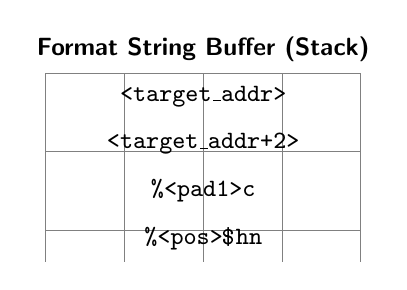
\begin{tikzpicture}[x=1cm,y=0.6cm, font=\sffamily\small]
  % Stack grid
  \draw[step=1cm,gray,very thin] (0,0) grid (4,-4);
  \node at (2,0.5) {\textbf{Format String Buffer (Stack)}};
  
  \node at (2,-0.5) {\texttt{<target\_addr>}};
  \node at (2,-1.5) {\texttt{<target\_addr+2>}};
  \node at (2,-2.5) {\texttt{\%<pad1>c}};
  \node at (2,-3.5) {\texttt{\%<pos>\$hn}};
\end{tikzpicture}
\caption{Memory layout showing the format string exploiting \texttt{\%hn} to perform a staged arbitrary write.}
\label{fig:fmt_staged_write}
\end{figure}

A generalized structure for a 16-bit-staged format string exploit looks like this (assuming the lower value is smaller than the higher value):

\begin{verbatim}
<target_addr><target_addr+2>
%<lower_value - length_of_targets>c
%<pos>$hn
%<higher_value - lower_value>c
%<pos+1>$hn
\end{verbatim}

\textbf{Handling Overflows:} If the second half is numerically smaller than the first half, the attacker relies on integer overflow. Because \texttt{\%hn} only writes the lower 16 bits, if the counter is incremented past $65,535$ (e.g., reaching \texttt{0x14241}), the \texttt{\%hn} placeholder will seamlessly write \texttt{0x4241}. Thus, the attacker simply adds $65,536$ to the smaller target value to compute the positive difference needed for the second padding.

\section{Targets for Overwriting}
With a robust arbitrary write primitive, an attacker can hijack the execution flow by overwriting key function pointers:
\begin{itemize}
    \item \textbf{Saved Return Address (Saved EIP):} Overwriting the return address on the stack. The challenge is locating the exact stack frame address reliably, making it similar to a basic stack overflow.
    \item \textbf{Global Offset Table (GOT):} A highly reliable target. The GOT stores dynamically resolved function pointers (like \texttt{exit()} or \texttt{printf()}). Overwriting a GOT entry allows the attacker to intercept subsequent library calls across the entire binary.
    \item \textbf{C Library Hooks:} such as \texttt{\_\_malloc\_hook} or \texttt{\_\_free\_hook}.
    \item \textbf{Exception Handlers:} Such as Windows SEH (Structured Exception Handling) chains.
\end{itemize}

\section{Countermeasures}

\begin{tcolorbox}[colback=red!5!white,colframe=red!75!black,title=Exam Insight]
You may be asked to analyze the bypass of memory mitigations like ASLR or Stack Canaries. A standard technique discussed in exams is using a Format String vulnerability to leak memory (such as a stack canary or a libc base address) before executing a secondary exploit like a Buffer Overflow.
\end{tcolorbox}

Modern development environments deploy several countermeasures to mitigate format string vulnerabilities:
\begin{itemize}
    \item \textbf{Compiler Warnings:} Modern compilers (\texttt{gcc}, \texttt{clang}) throw warnings (e.g., \texttt{-Wformat-security}) when a formatting function is called with a variable format string instead of a string literal.
    \item \textbf{Source Code Auditing:} Ensuring \texttt{printf(str)} is always rewritten securely as \texttt{printf("\%s", str)}.
    \item \textbf{Dynamic Mitigations:} such as \texttt{FormatGuard}, or patches to the C standard library (\texttt{libc}) that count the expected arguments and verify they match the placeholders. Furthermore, modern \texttt{libc} implementations will abort execution if the format string contains \texttt{\%n} directives and the format string resides in writable memory.
\end{itemize}

\section{Conclusion}
Format string bugs are powerful memory corruption vulnerabilities. While exploiting them requires precise mathematical calculations of offsets and paddings, the resulting exploitation provides a robust, Turing Complete arbitrary read/write primitive. By mastering direct parameter access, the \texttt{\%n} specifier, and multi-stage writes with \texttt{\%hn}, an attacker gains complete control over process execution.


% Chapter 8: Web Application Security
\chapter{Web Application Security}

\section{Introduction}
Web applications have become the dominant paradigm for software delivery, powering everything from corporate intranets to cloud-based Software as a Service (SaaS) offerings. Due to their ubiquity and the fact that they are often exposed to the public internet, they present a prime target for malicious actors.

At the foundation of web applications lies HTTP (Hypertext Transfer Protocol), a stateless protocol designed for document retrieval rather than complex application state management. Emulating state and enforcing robust authentication on top of a fundamentally stateless and text-based protocol introduces numerous security challenges. 

A typical web application follows a 3-tier architecture:
\begin{enumerate}
    \item \textbf{Presentation Tier (Client):} Usually a web browser communicating via HTTP.
    \item \textbf{Logic Tier (Application Server):} Processes requests, implements business logic, and generates dynamic content.
    \item \textbf{Data Tier (Database Server):} Stores and retrieves persistent data.
\end{enumerate}

\subsection{The Untrustworthy Client}
The golden rule of web application security is that \textbf{the client is never trustworthy}. 
Developers often build applications assuming that the client will interact with the application exactly as intended---for instance, clicking a button to generate a specific, well-formed \texttt{GET} or \texttt{POST} request. Attackers, however, operate under a different mindset. They understand that the client is fully under their control, and they can manually craft any HTTP request with arbitrary parameters, headers, and payloads, completely bypassing client-side restrictions.

Because HTTP is a plain-text protocol, crafting custom requests is trivial using tools like \texttt{curl} or intercepting proxies. Consequently, relying on client-side validation (e.g., JavaScript input checks) is entirely ineffective for security. Every piece of data originating from the client---including URL parameters, form fields, headers, and cookies---must be treated as malicious and strictly validated on the server side.

\section{Input Validation and Filtering}
To defend against malicious input, applications must employ robust filtering mechanisms. Validation typically follows a sequence of techniques:
\begin{enumerate}
    \item \textbf{Whitelisting:} Defining a strict set of allowed characters or patterns and rejecting everything else.
    \item \textbf{Blacklisting:} Identifying and discarding known-bad inputs or characters.
    \item \textbf{Escaping (or Encoding):} Transforming special characters into a safe representation (e.g., HTML entities) so they are treated as data rather than executable code.
\end{enumerate}

As a fundamental principle, \textbf{whitelisting is vastly superior to blacklisting}. Attackers are endlessly creative; it is virtually impossible to anticipate and blacklist every possible malicious payload, especially when considering obfuscation techniques and evolving specifications.

\subsection{The Pitfalls of Blacklisting}
Consider the task of preventing malicious JavaScript execution (Cross-Site Scripting, or XSS) by blacklisting the \texttt{<SCRIPT>} tag. An attacker could bypass this filter using various techniques:
\begin{itemize}
    \item Using alternative tags like \texttt{<APPLET>}, \texttt{<IFRAME>}, or \texttt{<OBJECT>}.
    \item Exploiting event handlers such as \texttt{<img src="x" onerror="alert(1)">} or \texttt{<svg onload="alert(1)">}.
    \item Leveraging the \texttt{javascript:} URL schema in \texttt{href} or \texttt{src} attributes.
    \item Utilizing HTML entities or hex encodings to obfuscate the payload (e.g., \texttt{\&\#09;}, \texttt{\%0a}).
    \item Exploiting parser quirks in specific browsers.
\end{itemize}
Because the environment is so complex and constantly changing, blacklisting is doomed to fail. A robust defense relies on whitelisting and proper contextual escaping.

\section{Cross-Site Scripting (XSS)}
\begin{tcolorbox}[colback=blue!5!white,colframe=blue!75!black,title=Exam Insight]
For XSS, be prepared to identify vulnerabilities in provided source code. You will typically be asked to fill out a table identifying the vulnerability type, specifying the exact vulnerable lines and variables, and explaining how to properly fix or sanitize them. Furthermore, you must know how to write the final payload/code to reproduce specific attacks, such as Reflected, Stored, or DOM-based XSS.
\end{tcolorbox}
Cross-Site Scripting (XSS) is a widespread vulnerability that occurs when an application includes untrusted data in a web page without proper validation or escaping. This flaw allows an attacker to execute malicious client-side scripts (typically JavaScript) within the victim's browser.

XSS is generally categorized into three types:
\begin{itemize}
    \item \textbf{Stored XSS (Persistent):} The malicious payload is permanently stored on the target server (e.g., in a database backing a forum or comment section). When a victim navigates to the affected page, the payload is served and executed.
    \item \textbf{Reflected XSS (Non-Persistent):} The malicious payload is embedded in a crafted URL or request. The server receives the input and immediately "reflects" it back in its response. The payload is executed when the victim clicks the crafted link.
    \item \textbf{DOM-based XSS:} The vulnerability exists entirely within the client-side code. The server may not even process the malicious payload. Instead, a vulnerable JavaScript function on the page reads data from an attacker-controllable source (like the URL fragment) and dangerously updates the Document Object Model (DOM).
\end{itemize}

\subsection{The Power of XSS and Same Origin Policy}
A common misconception is that JavaScript executes in a secure sandbox, limiting its potential harm. In reality, XSS is devastating because it effectively bypasses the \textbf{Same Origin Policy (SOP)}.

The SOP is a fundamental security mechanism implemented by browsers that restricts how a document or script loaded from one origin can interact with a resource from another origin. However, because the injected XSS payload is served from the trusted origin, it executes with the full privileges of the application. 

An attacker can use XSS to:
\begin{itemize}
    \item Steal session cookies, leading to full account compromise (Session Hijacking).
    \item Perform unauthorized actions on behalf of the user.
    \item Access and exfiltrate sensitive information displayed on the page.
    \item Perform Drive-by Downloads to infect the victim's machine.
\end{itemize}

\subsection{Content Security Policy (CSP)}
Content Security Policy (CSP) is an added layer of security that helps mitigate XSS and data injection attacks. It is a W3C specification that allows site administrators to declare approved sources of content that the browser may load. 

CSP is delivered via HTTP response headers (e.g., \texttt{Content-Security-Policy: script-src 'self' https://trusted.com}). It can restrict where scripts can be loaded from, disable inline execution, and control other resource types.

While CSP is a powerful defense-in-depth mechanism, its adoption is slow due to practical challenges. Strict policies can break existing functionality, especially on legacy sites relying on inline scripts. Keeping policies updated in modern, dynamic web applications is complex, and certain browser extensions can interfere with CSP enforcement. Furthermore, research has shown that many deployed CSPs are overly permissive and easily bypassed.

\section{SQL Injection}
\begin{tcolorbox}[colback=blue!5!white,colframe=blue!75!black,title=Exam Insight]
SQLi exam questions frequently require identifying vulnerabilities in source code by filling out a structured table. You will need to point out the specific vulnerable lines and variables, and explain the appropriate fixes (e.g., implementing Prepared Statements). Additionally, expect to write the exact payloads required to reproduce specific attacks, particularly Blind and UNION-based SQL injections.
\end{tcolorbox}
SQL Injection (SQLi) occurs when user-supplied input is directly concatenated into database query strings without proper sanitization or parameterization. This allows an attacker to alter the structure of the SQL query, effectively tricking the database into executing unintended commands.

\subsection{Exploitation Scenarios}
Consider a vulnerable login query:
\begin{verbatim}
SELECT * FROM Users WHERE username='[USER_INPUT]' AND password='[PWD_INPUT]';
\end{verbatim}

\textbf{Authentication Bypass:} An attacker can inject \texttt{admin' -- } into the username field. The resulting query becomes:
\begin{verbatim}
SELECT * FROM Users WHERE username='admin' -- ' AND password='...';
\end{verbatim}
The \texttt{--} comments out the rest of the query, successfully logging the attacker in as 'admin' without requiring a password.

\textbf{Tautologies:} If the attacker doesn't know a valid username, they can inject \texttt{' OR '1'='1}:
\begin{verbatim}
SELECT * FROM Users WHERE username='' OR '1'='1' ...
\end{verbatim}
This forces the query to return all rows, frequently resulting in a successful login as the first user in the table.

\textbf{Data Exfiltration via UNION:} Attackers can use the \texttt{UNION} operator to append results from entirely different tables to the original query's output, provided the column structures match.

\textbf{Blind SQL Injection:} If the application does not display database errors or query results directly, attackers can still extract data. By injecting queries that ask true/false questions (e.g., "Is the first letter of the password 'A'?"), the attacker observes the application's behavior (e.g., differences in page content or response time) to infer the data character by character.

\subsection{Mitigating Code Injection}
The core conflict causing injection vulnerabilities is the mixing of data and control instructions within a single parser context (whether it's an SQL interpreter or an HTML parser).

To prevent SQL injection, developers must fundamentally separate data from code using \textbf{Prepared Statements} (Parametrized Queries). With prepared statements, the query structure is defined beforehand, and user inputs are supplied strictly as data parameters. The database driver ensures that these parameters are never interpreted as executable SQL commands, completely neutralizing the vulnerability. Additional defenses include least-privilege database accounts and input validation.

\section{Information Leaks and Parameter Tampering}
\begin{tcolorbox}[colback=blue!5!white,colframe=blue!75!black,title=Exam Insight]
Be prepared to write payloads to reproduce Path Traversal attacks. You may be required to demonstrate how to manipulate URL parameters to access unauthorized files on the server (e.g., using sequences like \texttt{../../../../etc/passwd}). You should clearly explain the steps to achieve the exploit.
\end{tcolorbox}
Applications must handle errors gracefully without revealing sensitive internal details. Detailed debug traces and verbose error messages (Freudian slips) can leak structural information about the database, server software versions, and internal file paths, which attackers can leverage.

\textbf{URL Parameter Tampering} involves manipulating parameters in the GET request or POST body to access unauthorized data. A classic example is \textbf{Directory Traversal} (or Path Traversal), where an attacker manipulates a file path parameter (e.g., \texttt{file=../../../../etc/passwd}) to access arbitrary files on the server's filesystem outside the intended web root.

\section{Session Management and Authentication}
Because HTTP is stateless, applications must implement custom session management to track authenticated users across multiple requests.

\subsection{Password Security}
Passwords must never be stored in plain text. They should be securely hashed and salted to slow down brute-force and dictionary attacks, mitigating the impact of a database breach. Additionally, account recovery mechanisms (password resets) require careful design to avoid introducing new vulnerabilities (e.g., relying solely on easily guessable security questions). Brute-forcing protection should involve account lockouts or rate limiting, though simplistic IP blocking can lead to Denial of Service (DoS) issues due to shared proxies or NATs.

\subsection{Cookies and Session Hijacking}
Sessions are typically implemented using Session IDs stored in client-side \textbf{Cookies}. When a user authenticates, the server generates a unique Session ID and sends it via a \texttt{Set-Cookie} header. The browser then automatically includes this cookie in all subsequent requests to that domain.

Session IDs must be unpredictable to prevent attackers from guessing valid tokens and impersonating users. Furthermore, session stealing (hijacking) via XSS is a critical threat. To mitigate this, sensitive cookies should employ the \texttt{HttpOnly} flag, which prevents client-side JavaScript from accessing the cookie, severely limiting the impact of an XSS vulnerability on session integrity.

\section{Cross-Site Request Forgery (CSRF)}
\begin{tcolorbox}[colback=blue!5!white,colframe=blue!75!black,title=Exam Insight]
CSRF questions often ask you to identify the vulnerability within a given source code snippet (often filling out a vulnerability table with lines, variables, and fixes) and provide the final payload or code to reproduce the attack. For instance, you might need to craft a malicious HTML form that automatically submits a forged cross-site request to the vulnerable endpoint when visited by the victim.
\end{tcolorbox}
Cross-Site Request Forgery (CSRF) is an attack that forces an authenticated user to execute unwanted, state-changing actions on a web application.

The attack exploits the fact that browsers automatically include ambient credentials (like session cookies) with every request made to a domain. If a victim visits a malicious site while authenticated to their bank, the malicious site can trigger a hidden request (e.g., via an invisible form submission or an image tag) to the bank's servers, transferring funds to the attacker. Since the request includes the victim's valid session cookie, the bank processes it legitimately.

\subsection{CSRF Mitigation}
\begin{itemize}
    \item \textbf{Anti-CSRF Tokens:} The server generates a unique, cryptographically strong random token for the user's session. This token is included as a hidden field in sensitive HTML forms. When the form is submitted, the server verifies that the submitted token matches the expected token for that session. Because an attacker cannot read the token from the target site (due to the Same Origin Policy), they cannot forge a valid request. \textbf{Note:} These tokens must not be stored in cookies alone, as that defeats the purpose.
    \item \textbf{SameSite Cookies:} A modern defense mechanism where the \texttt{SameSite} attribute is added to the cookie declaration. By setting \texttt{SameSite=Strict} or \texttt{SameSite=Lax}, the browser restricts when cookies are sent in cross-origin requests, effectively neutralizing CSRF attacks at the browser level.
\end{itemize}

\section{Conclusion}
Web application security is a complex field characterized by an asymmetric battle between developers and attackers. Securing modern applications requires a defense-in-depth approach, treating all client input as hostile, strictly separating code from data, and properly implementing authentication and session management.

\begin{tcolorbox}[colback=blue!5!white,colframe=blue!75!black,title=Chapter Summary]
This chapter explores the foundational concepts and critical vulnerabilities associated with modern web applications. Key topics include the untrustworthy nature of the client, input validation techniques (whitelisting vs. blacklisting), Cross-Site Scripting (XSS), SQL Injection (SQLi), Path Traversal, and Cross-Site Request Forgery (CSRF). Mitigations such as Prepared Statements, Content Security Policy (CSP), and robust session management are also discussed in detail.
\end{tcolorbox}

\begin{table}[h!]
    \centering
    \begin{tabular}{|l|p{10cm}|}
        \hline
        \textbf{Vulnerability} & \textbf{Description} \\ \hline
        XSS & Execution of malicious client-side scripts within the victim's browser. \\ \hline
        SQL Injection & Altering database queries via unsanitized user input. \\ \hline
        Path Traversal & Manipulating file paths to access unauthorized files. \\ \hline
        CSRF & Forcing an authenticated user to execute unwanted actions. \\ \hline
    \end{tabular}
    \caption{Common Web Application Vulnerabilities}
    \label{tab:web_vulns}
\end{table}


% Chapter 9: Network Protocol Attacks
\chapter{Network Protocol Attacks}

This chapter covers the fundamental vulnerabilities inherent in standard network protocols, primarily stemming from the lack of built-in strong authentication.

\begin{table}[ht]
\centering
\begin{tabular}{|l|p{10cm}|}
\hline
\textbf{Attack Category} & \textbf{Description \& Examples} \\
\hline
Denial of Service (DoS) & Targets availability via resource exhaustion (e.g., Ping of Death, SYN Flood, Smurf Attack). \\
Sniffing & Targets confidentiality by intercepting traffic (e.g., MAC Flooding, ARP Spoofing). \\
Spoofing \& Hijacking & Targets integrity/authenticity (e.g., IP Spoofing, TCP Session Hijacking, MITM). \\
Application Layer & Exploits application protocols (e.g., DNS Cache Poisoning, DHCP Poisoning). \\
Network Control & Exploits control protocols (e.g., ICMP Redirect, Route Mangling). \\
\hline
\end{tabular}
\caption{Summary of Network Protocol Attacks}
\end{table}

\section{Introduction to Network Protocols and Layering}

The Internet is a complex interconnection of various physical media, topologies, and administrative domains. To manage this complexity, network architectures adopt a layered approach. The two most prominent models are the ISO/OSI (Open Systems Interconnection) reference model and the TCP/IP stack.

While the OSI model defines seven layers (Physical, Data Link, Network, Transport, Session, Presentation, Application), the TCP/IP model condenses these into four practical layers: Network Access (or Link), Internet, Transport, and Application. This layering allows for abstraction, meaning a protocol at a specific layer only needs to communicate with its counterpart on another machine, relying on the layers below it to handle the actual transmission.

Data transmission across these layers involves \textbf{encapsulation}. As data moves down the stack from the application layer to the physical layer, each protocol adds its own header (and sometimes a trailer). For instance, an HTTP message (Application) is encapsulated in a TCP segment (Transport), which is encapsulated in an IP datagram (Internet), which is finally encapsulated in an Ethernet frame (Data Link).

\subsection{Addressing Systems}

Different layers employ distinct addressing structures to identify nodes and services:
\begin{itemize}
    \item \textbf{Data Link Layer (MAC Address):} Used primarily in Ethernet and Wi-Fi networks, the Media Access Control (MAC) address is a 48-bit globally unique identifier ``burnt'' into the Network Interface Card (NIC).
    \item \textbf{Internet Layer (IP Address):} The Internet Protocol (IP) address uniquely identifies a host across the global network (or within a private network using RFC 1918 addresses). It is a logical address used for routing packets across different networks.
    \item \textbf{Transport Layer (Port):} Ports identify specific services or applications running on a host. For example, port 80 typically denotes HTTP traffic, while port 443 denotes HTTPS.
\end{itemize}

\section{Taxonomy of Typical Network Attacks}

\begin{tcolorbox}[colback=blue!5!white,colframe=blue!75!black,title=Exam Insight]
For any of these attack categories, exam questions often ask you to analyze network packet captures/logs to determine the IP addresses of the attacker and the victim, and identify the attacker's main goal from traffic traces.
\end{tcolorbox}

Network attacks generally exploit the lack of authentication or fundamental design flaws in early protocol specifications. They can be broadly classified into three categories based on the security principles they violate:

\begin{enumerate}
    \item \textbf{Denial of Service (DoS):} Targets \textit{availability}. The goal is to render a service or resource unavailable to legitimate users.
    \item \textbf{Sniffing:} Targets \textit{confidentiality}. It involves the unauthorized interception and reading of network packets traversing the medium.
    \item \textbf{Spoofing:} Targets \textit{integrity and authenticity}. It involves forging network packets to masquerade as another host or service.
\end{enumerate}

\section{Denial of Service (DoS) Attacks}

Denial of Service attacks aim to exhaust the resources of a target system, such as bandwidth, memory, or CPU cycles.

\subsection{Killer Packets}
Early DoS attacks relied on sending malformed packets that exploited bugs or memory errors in network stack implementations. These are often referred to as ``Killer Packets.''

\begin{itemize}
    \item \textbf{Ping of Death:} Exploited the maximum legal length of an IP packet (65,535 octets). By sending oversized, fragmented ICMP echo requests, the target's operating system would crash or freeze during the reassembly process due to buffer overflows.
    \item \textbf{Teardrop Attack:} Exploited vulnerabilities in TCP/IP fragmentation reassembly. The attacker sends fragmented packets with overlapping offsets. When the target attempts to reconstruct the original packet, the overlapping offsets cause the kernel to hang or crash. This affected many major operating systems in the late 90s and reappeared in 2009 affecting SMB in Windows Vista.
    \item \textbf{Land Attack:} A carefully crafted packet is sent where both the source and destination IP addresses are set to the target's IP address, and the SYN flag is set. This causes the target's TCP stack to attempt to establish a connection with itself, creating an infinite loop that locks up the system.
\end{itemize}

\subsection{SYN Flood Attack}

\begin{tcolorbox}[colback=blue!5!white,colframe=blue!75!black,title=Exam Insight]
Exam questions often ask you to propose network mitigations. Be prepared to suggest and explain mitigations like SYN-cookies to prevent SYN Flood attacks.
\end{tcolorbox}

The SYN Flood is a classic resource exhaustion attack that exploits the TCP three-way handshake.

Normally, a TCP connection is established as follows:
\begin{enumerate}
    \item Client sends a \texttt{SYN} packet to the Server.
    \item Server allocates memory in its queue, replies with a \texttt{SYN-ACK}, and leaves the connection in a ``half-open'' state.
    \item Client completes the handshake with an \texttt{ACK}.
\end{enumerate}

In a SYN Flood attack, the attacker generates a high volume of \texttt{SYN} requests using \textit{spoofed} source IP addresses. The server receives these requests, allocates resources in its connection queue, and sends \texttt{SYN-ACK} packets to the spoofed addresses. Because the spoofed addresses either do not exist or are not initiating a connection, the final \texttt{ACK} is never sent back. The server's queue quickly fills up with these half-open connections, preventing legitimate clients from establishing new connections.

\textbf{Mitigation: SYN Cookies.} To mitigate SYN floods, servers can use SYN cookies. Instead of allocating memory for a half-open connection upon receiving a \texttt{SYN}, the server calculates a cryptographic hash (the ``cookie'') based on the connection details and the TCP sequence number, and sends it back in the \texttt{SYN-ACK}. The server discards the state. If the client is legitimate, it will reply with an \texttt{ACK} containing the incremented sequence number. The server recalculates the hash to verify the cookie and then allocates memory for the fully established connection.

\subsection{Distributed Denial of Service (DDoS)}

A DDoS attack magnifies the impact of a DoS attack by coordinating multiple compromised machines to target a single victim.

\textbf{Botnets:} Attackers often use botnets---networks of compromised computers (bots) infected with malware---controlled via a Command and Control (C\&C) infrastructure. The botmaster can command thousands of bots to simultaneously flood a target.

\textbf{Smurf Attack:} An early form of DDoS and amplification. The attacker sends an ICMP Echo Request (\texttt{ping}) to a network's broadcast address (e.g., \texttt{1.1.1.255}), but spoofs the source IP address to be the victim's IP. All hosts on the broadcast network reply to the victim simultaneously, overwhelming its bandwidth.

\textbf{Amplification Attacks:} These attacks exploit protocols that yield a response much larger than the initial request (a high Bandwidth Amplification Factor or BAF). The attacker sends a small request with a spoofed source IP (the victim's IP) to a vulnerable server (e.g., NTP, DNS, SNMP). The server sends the massive response to the victim. For instance, an NTP ``monlist'' request can result in an amplification factor of over 500x.

\section{Sniffing and Local Area Network Attacks}

Normally, a Network Interface Card (NIC) only processes packets destined for its own MAC address (or broadcast addresses). However, if placed in \textbf{promiscuous mode}, the NIC will pass all traffic it sees on the wire up to the operating system, allowing an attacker to ``sniff'' or eavesdrop on the network.

\subsection{Hubs vs. Switches}
In older networks using shared media (like BNC cables) or \textbf{hubs}, all traffic is broadcasted to every connected device, making sniffing trivial. Modern networks use \textbf{switches}, which selectively forward frames only to the port where the destination MAC address resides. Switches use a \textbf{CAM (Content Addressable Memory) table} to cache the mapping of MAC addresses to physical ports. While switches improve performance and offer a baseline of security against casual sniffing, they are vulnerable to specific attacks.

\subsection{MAC Flooding}

\begin{tcolorbox}[colback=blue!5!white,colframe=blue!75!black,title=Exam Insight]
When analyzing network packet captures (like CAM flooding/MAC flooding), you may need to identify the type of attack taking place and describe its steps. Additionally, you might be asked to propose network mitigations such as Port Security to prevent it.
\end{tcolorbox}

An attacker can overwhelm a switch's CAM table by generating thousands of spoofed frames with random source MAC addresses in a matter of seconds (using tools like \texttt{macof}). Once the CAM table is full, the switch cannot learn new MAC addresses and defaults to ``fail-open'' behavior---it begins broadcasting all incoming frames to all ports, effectively turning the switch into a hub and allowing the attacker to sniff all traffic.
\textbf{Mitigation:} Port Security features can limit the number of MAC addresses allowed on a single switch port.

\subsection{ARP Spoofing and Cache Poisoning}

\begin{tcolorbox}[colback=blue!5!white,colframe=blue!75!black,title=Exam Insight]
ARP Spoofing/Poisoning is a frequent topic in network packet capture analysis questions. You must be able to identify it from a trace and describe its steps in detail.
\end{tcolorbox}

The Address Resolution Protocol (ARP) translates 32-bit IPv4 addresses into 48-bit MAC addresses. When a host needs to find the MAC address for an IP, it broadcasts an ARP Request. The owner of the IP replies with an ARP Reply.

\textbf{Vulnerability:} ARP is entirely \textit{unauthenticated} and stateless. Hosts operate on a ``first come, first trusted'' basis and will aggressively cache any ARP replies they receive.

An attacker can send forged, unsolicited ARP Replies (Gratuitous ARP) to a victim, falsely claiming that the attacker's MAC address is associated with a specific IP address (usually the default gateway). The victim caches this poisoned record. Consequently, all traffic destined for the gateway is sent to the attacker instead. The attacker can then sniff, modify, or drop the packets before forwarding them to the real gateway.

\subsection{Spanning Tree Protocol (STP) Abuse}
The Spanning Tree Protocol (STP, 802.1d) prevents routing loops in switched networks by electing a root node and disabling redundant links. Switches elect the root node by exchanging Bridge Protocol Data Units (BPDUs). Because BPDUs are not authenticated, an attacker can broadcast forged BPDUs with the highest priority, forcing the network to elect the attacker's machine as the root bridge. This alters the network topology, causing large volumes of traffic to flow through the attacker's machine for interception.

\section{IP Spoofing and Session Hijacking}

\subsection{IP Spoofing (UDP/ICMP vs. TCP)}
The source IP address in an IP packet header is not authenticated by the protocol itself. Changing the source IP is trivial. For connectionless protocols like UDP or ICMP, the spoofed packet simply reaches the destination, and any response goes to the spoofed source. This is known as \textbf{blind spoofing} if the attacker cannot intercept the return traffic.

For TCP, which is connection-oriented, spoofing is significantly harder due to the required three-way handshake and Sequence Numbers.

\subsection{TCP Sequence Number Guessing}
TCP uses sequence numbers to order packets and ensure reliable delivery. When establishing a connection, a semi-random Initial Sequence Number (ISN) is chosen. 

If an attacker attempts a blind spoofing attack (where they cannot sniff the target's replies), they must accurately guess the ISN sent by the server in the \texttt{SYN-ACK} packet to successfully forge the final \texttt{ACK} and establish the connection. Furthermore, the actual spoofed host must be prevented from receiving the server's \texttt{SYN-ACK}, otherwise, it will respond with an \texttt{RST} (Reset) packet, terminating the connection.

Historically (e.g., the famous Kevin Mitnick attack in 1995), operating systems used highly predictable ISN generation algorithms, making this attack feasible. Modern OSes use cryptographically secure random ISNs, making blind TCP spoofing exceedingly difficult.

\subsection{TCP Session Hijacking}

\begin{tcolorbox}[colback=blue!5!white,colframe=blue!75!black,title=Exam Insight]
Exam questions may present packet logs and ask you to identify TCP session hijacking. You will need to describe the steps the attacker takes, such as predicting sequence numbers or disrupting the original connection.
\end{tcolorbox}

If the attacker is on the same local network or path and can sniff the traffic, they don't need to guess sequence numbers. 

In a TCP Session Hijacking attack:
\begin{enumerate}
    \item The attacker (C) sniffs an established TCP connection between Client (A) and Server (B), observing the current sequence and acknowledgment numbers.
    \item C disrupts A's connection (e.g., by executing a targeted DoS or SYN flood against A).
    \item C injects a packet to B, spoofing A's IP address and using the correct next sequence number. B accepts the packet as legitimate data from A.
\end{enumerate}

\subsection{Man In The Middle (MITM)}
A MITM attack is a broad category where the attacker inserts themselves between two communicating parties, impersonating each to the other. If an attacker successfully executes ARP spoofing to become the gateway, they achieve a physical/logical MITM position, allowing them full control to intercept, modify, or inject traffic seamlessly.

\section{Application Layer Protocol Attacks}

\subsection{Domain Name System (DNS) Attacks}

\begin{tcolorbox}[colback=blue!5!white,colframe=blue!75!black,title=Exam Insight]
DNS Cache Poisoning is often featured in packet analysis questions. Be ready to identify the attack and explain its mechanism, such as spoofing the Transaction ID and flooding the local server with forged responses.
\end{tcolorbox}

DNS translates human-readable domain names (e.g., \texttt{www.google.com}) into IP addresses. It operates as a distributed, hierarchical database primarily over UDP port 53. Because standard DNS queries and responses are unauthenticated, it is highly vulnerable to spoofing.

\textbf{DNS Cache Poisoning:}
When a client asks its local, non-authoritative DNS server for a domain it doesn't know, the server performs a recursive query on behalf of the client. 
\begin{enumerate}
    \item The attacker forces the local DNS server to resolve a target domain.
    \item The local server contacts the authoritative nameserver.
    \item Before the genuine authoritative server can reply, the attacker floods the local server with forged DNS responses containing a malicious IP address.
    \item To be accepted, the forged response must match the 16-bit \textbf{Transaction ID} (and UDP source port) of the original request. Attackers use brute force or vulnerabilities (like the Dan Kaminsky flaw discovered in 2008, which exploited predictable port allocation and requested random subdomains) to guess these parameters.
    \item The local DNS server accepts the forged response, caches the poisoned record, and subsequently redirects all legitimate clients to the attacker's malicious site.
\end{enumerate}

\subsection{Dynamic Host Configuration Protocol (DHCP) Attacks}
DHCP dynamically assigns IP addresses, subnet masks, default gateways, and DNS servers to clients joining a network. The process involves a \texttt{DISCOVER}, \texttt{OFFER}, \texttt{REQUEST}, and \texttt{ACK} exchange over UDP.

\textbf{DHCP Poisoning (Rogue DHCP Server):}
Since DHCP is unauthenticated, an attacker can set up a rogue DHCP server on the local network. When a new client broadcasts a \texttt{DHCP DISCOVER} message, the attacker races to send a \texttt{DHCP OFFER} before the legitimate server. If the client accepts the rogue offer, the attacker can provision the client with a malicious IP address, a rogue DNS server (facilitating phishing), and set the attacker's machine as the default gateway (facilitating a MITM attack).

\section{Network Control Protocol Attacks}

\subsection{Internet Control Message Protocol (ICMP)}

\begin{tcolorbox}[colback=blue!5!white,colframe=blue!75!black,title=Exam Insight]
Questions involving ICMP Redirect often require you to identify the attack from network logs and explain the steps taken to trick a host into routing traffic maliciously.
\end{tcolorbox}

ICMP is designed for sending error messages and operational information (e.g., \texttt{Echo Request/Reply} for ping, \texttt{Destination Unreachable}, \texttt{Time Exceeded}).

\textbf{ICMP Redirect Attack:}
An \texttt{ICMP Redirect} message is used by a router to inform a host that a more optimal route exists for a specific destination. An attacker can forge an ICMP Redirect packet to trick a host into routing its traffic through the attacker's machine or into a black hole (DoS). This attack relies on the fact that ICMP messages have weak authentication (they merely include the IP header and the first 8 bytes of the original datagram). The success of this attack often depends on the host OS; many modern operating systems ignore ICMP redirects by default.

\subsection{Route Mangling}
Routers use dynamic routing protocols (like RIP, OSPF, EIGRP, BGP) to learn and share network topologies. Many older protocols (RIP, OSPF) have weak or optional authentication mechanisms. Even in protocols where authentication is available (like BGP), it is historically underutilized. 

An attacker who gains access to a router or can inject routing updates can ``mangle'' the routing tables. By announcing false, highly attractive routes (e.g., a very specific subnet prefix), the attacker can hijack vast amounts of Internet traffic, redirecting it for interception or causing massive, wide-scale Denial of Service (as seen in various BGP hijacking incidents).

\section{Conclusion}

\begin{tcolorbox}[colback=blue!5!white,colframe=blue!75!black,title=Exam Insight]
A common exam exercise involves writing stateful firewall rules based on a given network topology and specific security requirements, or proposing topology changes (like adding a DMZ, VPN, or NAT) to prevent specific attacks.
\end{tcolorbox}

Network protocols were largely designed with functionality and resilience in mind, often in environments where trust was assumed. The lack of strong, built-in cryptographic authentication at the lower layers (Link, Internet, Transport) exposes modern networks to a wide array of attacks. From resource exhaustion via DoS to sophisticated MITM and cache poisoning techniques, attackers exploit inherent structural weaknesses. Securing a network requires a defense-in-depth approach, implementing security controls, stateful inspection, and cryptographic protocols (like IPsec, DNSSEC, and TLS) layered on top of the foundational protocols.


% Chapter 10: Secure Network Architectures
\chapter{Secure Network Architectures}
\label{ch:secure_network_architectures}

\textbf{Chapter Summary:} This chapter covers the fundamental concepts of securing network perimeters using firewalls and Virtual Private Networks (VPNs). It details firewall taxonomies (stateless, stateful, circuit-level, and application proxies), their interaction with NAT, and how network architectures like the Demilitarized Zone (DMZ) are used to isolate public-facing servers from private networks. Finally, it explores VPN technologies for secure remote access over public networks.

\begin{table}[h]
\centering
\begin{tabular}{|l|p{10cm}|}
\hline
\textbf{Topic} & \textbf{Description} \\
\hline
Firewalls & Network access control systems acting as single enforcement points. \\
\hline
Packet Filters & Stateless filters evaluate packets individually; stateful filters track connection states. \\
\hline
Application Proxies & Operate at the application layer for deep payload inspection. \\
\hline
DMZ & Semi-public zone hosting internet-facing servers to protect internal networks. \\
\hline
VPN & Encrypted, authenticated overlay connections over public networks. \\
\hline
\end{tabular}
\caption{Key Concepts of Secure Network Architectures}
\label{tab:secure_networks_summary}
\end{table}

\section{Introduction to Firewalls}

In the context of computer security, a \textbf{firewall} is a network access control system that verifies all the packets flowing through it. Its primary purpose is to act as a barrier between a trusted, screened network and untrusted outside networks, such as the Internet. To be effective, a firewall must serve as the single enforcement point between these networks; otherwise, its policies could be bypassed.

The main functions of a firewall typically include:
\begin{itemize}
    \item \textbf{IP Packet Filtering:} Inspecting incoming and outgoing packets and deciding whether to let them pass or drop them based on a set of predefined rules.
    \item \textbf{Network Address Translation (NAT):} Modifying network address information in packet headers while in transit across a traffic routing device.
\end{itemize}

\textit{A side note on grammar:} In IT, the correct term is ``firewall'' (one word), not ``fire wall''. In Italian context, the word is masculine (``un firewall'', not ``una firewall''). The term originally comes from construction, referring to a wall designed to partition a building and stop the spread of fire.

\subsection{Limitations of Firewalls}

Firewalls are powerful tools, but they are not omnipotent. A firewall checks \textit{all} the traffic flowing through it, but \textit{only} the traffic flowing through it. Consequently, firewalls are powerless against attacks that do not cross their path.

\begin{itemize}
    \item \textbf{Insider Attacks:} If a malicious actor is already inside the local network, the perimeter firewall cannot stop them from accessing internal resources, unless the internal network itself is partitioned with additional firewalls.
    \item \textbf{Unchecked Paths:} Firewalls cannot protect against alternate routes into the network that bypass the firewall entirely. For example, if a machine within the Local Area Network (LAN) is also connected to the Internet via a separate 4G/5G modem, it creates an unchecked path that completely bypasses the firewall's scrutiny.
\end{itemize}

\subsection{Firewalls as Attack Targets}

It is important to remember that a firewall is itself a computer, meaning it can have vulnerabilities and be compromised. However, most firewalls are single-purpose machines---often embedded appliances running specialized firmware. They usually offer few or no extraneous services, which significantly reduces their attack surface compared to a general-purpose operating system.

\subsection{Security Policies and Firewall Rules}

A firewall can be thought of as a strict ``bouncer at the door''; it simply applies the rules it has been given. If the rules are poorly configured, the firewall provides no protection.

Firewall rules are essentially the technical implementation of higher-level security policies. For instance, a security policy might state: \textit{``Clients are not allowed to download email from external servers.''} The corresponding firewall rule would block outbound connections on ports associated with POP3 or IMAP to external IP addresses.

Crucially, an effective security policy must be built on a \textbf{default deny} base. This means the underlying philosophy is ``deny all, except what is explicitly permitted''. Any traffic not explicitly allowed by a rule should be dropped.

\begin{tcolorbox}[colback=blue!5!white,colframe=blue!75!black,title=Exam Insight]
Expect questions where you must complete a table with stateful firewall rules based on a given network topology and specific security requirements. Remember to rely on the ``default deny'' base policy and carefully track the state of connections for inbound and outbound traffic flows.
\end{tcolorbox}

\section{Firewall Taxonomy}

Firewalls can be broadly classified based on their packet inspection capability, ranging from the network layer up to the application layer of the OSI model.

\begin{enumerate}
    \item \textbf{Network Layer Firewalls:}
    \begin{itemize}
        \item \textbf{Stateless Packet Filters:} Operate strictly at the network layer, examining each packet individually without memory of past packets.
        \item \textbf{Stateful Packet Filters (SPF):} Operate at the network and transport layers, tracking the state of active connections.
    \end{itemize}
    \item \textbf{Application Layer Firewalls:}
    \begin{itemize}
        \item \textbf{Circuit-Level Firewalls:} Operate between the transport and application layers, relaying TCP connections.
        \item \textbf{Application Proxies:} Operate at the application layer, understanding and inspecting the payload of specific protocols.
    \end{itemize}
\end{enumerate}

\subsection{Stateless Packet Filters}

Stateless packet filters process traffic on a strict packet-by-packet basis. They decode the IP header and parts of the TCP/UDP header, allowing rules to be based on:
\begin{itemize}
    \item Source and Destination IP addresses
    \item Source and Destination ports
    \item Protocol type (e.g., TCP, UDP, ICMP)
    \item IP options
\end{itemize}

Because they are \textbf{stateless}, they cannot track TCP connections. Each packet is evaluated in isolation. They also do not perform full payload inspection. Stateless packet filters are often found on routers (e.g., Access Control Lists or ACLs on Cisco devices).

\subsubsection{Expressiveness and Rule Structure}

The expressiveness of a stateless filter is limited to the fields it can decode. Rules define a condition and an associated reaction. If a packet matches the condition, the firewall executes the reaction, which could be to \textbf{allow}, \textbf{block} (drop or reject), \textbf{log}, or rate-limit the packet.

For example, using Linux \texttt{iptables} syntax:
\begin{itemize}
    \item \texttt{iptables -P INPUT DROP}: Sets the default policy to block all incoming packets.
    \item \texttt{iptables -A INPUT -d 10.0.0.1 -j ALLOW}: Allows incoming packets destined for 10.0.0.1.
    \item \texttt{iptables -A OUTPUT --dport 25 -j ALLOW}: Allows outgoing packets destined for port 25 (SMTP).
\end{itemize}

\subsubsection{The Problem with Stateless Filters}

A significant vulnerability of stateless filters is handling responses. If an internal client initiates a connection to an external web server, the firewall must allow the outgoing request. However, to receive the response, the firewall must also have a rule allowing incoming traffic from the web server. In a purely stateless setup, this often requires opening a wide range of inbound high ports to the entire Internet, severely weakening security.

\subsection{Stateful (Dynamic) Packet Filters}

Stateful packet filters improve upon stateless ones by keeping track of the \textbf{transport layer state machine}. For TCP connections, they monitor the three-way handshake: if a \texttt{SYN} packet is seen going out, the firewall expects a \texttt{SYN-ACK} to return.

By tracking the connection state in a ``state table,'' a stateful firewall can automatically allow incoming response packets that belong to an established connection \textit{without} requiring an explicit inbound allow rule. This makes the default deny rule much safer and easier to maintain.

\subsubsection{Advantages and Disadvantages}

\textbf{Advantages:}
\begin{itemize}
    \item \textbf{Safer Deny Rules:} No need to permanently open inbound ports for responses.
    \item \textbf{Better Expressiveness:} They can log and account for connections, not just individual packets.
    \item \textbf{Defragmentation and Reassembly:} They can reassemble fragmented packets before inspection, thwarting evasion techniques and attacks exploiting pathological fragmentation (e.g., the teardrop attack).
    \item \textbf{NAT Integration:} Network Address Translation is typically offered as an embedded feature.
\end{itemize}

\textbf{Disadvantages:}
\begin{itemize}
    \item \textbf{Resource Constraints:} Performance is bounded on a \textit{per-connection} basis rather than just a per-packet basis. Maintaining state consumes memory. The maximum number of simultaneous connections is a critical performance metric, making them susceptible to state exhaustion attacks (like SYN floods).
\end{itemize}

\subsubsection{Session Handling and NAT}

A \textbf{session} is an atomic, transport-layer exchange of application data between two hosts. Stateful firewalls track these sessions to perform NAT.

For \textbf{TCP}, tracking is straightforward because it is a connection-oriented protocol with explicit start (\texttt{SYN}) and end (\texttt{FIN}/\texttt{RST}) flags. When an internal client initiates a TCP connection, the firewall creates a NAT slot. It translates the internal IP and port to a public IP and port, and forwards the packet. When the \texttt{SYN-ACK} returns to the public IP/port, the firewall uses the NAT table to translate it back to the internal client.

\textbf{UDP}, however, is connectionless. The concept of a session does not strictly exist at the transport layer. To handle UDP over NAT, the stateful firewall must \textit{infer} a session. When an internal host sends a UDP packet, the firewall creates a NAT slot and starts a timer. If a response packet is received from the destination within a certain timeout (e.g., 2 minutes), it is considered part of the inferred ``session'' and translated back to the client.

\subsubsection{Application-Layer Inspection for NAT}

Some protocols embed network information (like IP addresses and ports) inside the application-layer payload. NAT breaks these protocols because it translates the headers but leaves the payload unmodified.

A classic example is \textbf{FTP (File Transfer Protocol)}. FTP uses two separate connections: a command channel (port 21) and a data channel (port 20 or dynamic).

\begin{itemize}
    \item \textbf{FTP Standard (Active) Mode:} The client connects to the server's port 21. When a file transfer is requested, the client sends a \texttt{PORT} command containing its IP address and a dynamically chosen listening port. The server then initiates a new connection back to the client's specified IP and port. 
    
    If the client is behind a NAT firewall, the IP in the \texttt{PORT} command is a private IP. The server cannot connect to it. Furthermore, the client-side firewall would block the incoming connection anyway. To fix this, a stateful firewall must inspect the FTP application layer, intercept the \texttt{PORT} command, rewrite the private IP/port to the firewall's public IP/port, and dynamically open a hole for the incoming data connection.

    \item \textbf{FTP Passive Mode:} To mitigate firewall issues, FTP Passive mode was introduced. The client sends a \texttt{PASV} command. The server responds with its IP and a dynamic port it is listening on. The \textit{client} then initiates the data connection to the server. This avoids the server needing to bypass the client's firewall, but now the server's firewall must dynamically open inbound ports based on the \texttt{PASV} response.
\end{itemize}

\section{Application Layer Firewalls}

Application layer firewalls operate higher up the OSI stack, providing deeper inspection at the cost of performance and transparency.

\subsection{Circuit-Level Firewalls (Legacy)}

Circuit-level firewalls relay TCP connections. The client explicitly connects to a specific TCP port on the firewall, which then initiates a second connection to the target server. They are essentially TCP-level proxies. Because the client must be aware of the proxy and intentionally route traffic to it, they are \textbf{not transparent}. 

A historical example is SOCKS.

\subsection{Application Proxies}

Application proxies operate similarly to circuit firewalls but possess an understanding of specific application-layer protocols (e.g., HTTP, SMTP). 

Because they understand the protocol, they can:
\begin{itemize}
    \item Inspect, validate, and manipulate protocol application data (e.g., rewriting HTTP frames, filtering ActiveX objects).
    \item Authenticate users before granting access.
    \item Apply highly granular filtering policies.
    \item Perform advanced logging.
    \item Conduct content filtering or scanning (e.g., anti-virus, anti-spam).
\end{itemize}

Like circuit firewalls, they are almost never transparent to clients, requiring client configuration (like configuring an HTTP Proxy in browser settings). Furthermore, each protocol requires its own dedicated proxy server software.

Application proxies can be deployed to protect internal clients (Forward Proxy) or to protect internal servers by acting as the public face of the service (\textbf{Reverse Proxy}). They are usually implemented on commercial off-the-shelf (COTS) operating systems rather than embedded firmware.

\section{Architectures for Secure Networks}

Firewalls enforce policies, but network architecture dictates where those policies are applied.

\subsection{Dual- or Multi-Zone Architectures}

The traditional perimeter defense model assumes the internal network is ``good'' and the external network is ``bad.'' However, there are scenarios where external access is necessary:
\begin{enumerate}
    \item External users need to access public resources (web servers, FTP servers, MX records).
    \item Remote employees need to access the corporate network.
\end{enumerate}

Mixing publicly accessible servers with internal client workstations on the same local network is highly insecure. If a public web server is compromised, the attacker immediately gains unrestricted access to the internal network.

The solution is to physically and logically separate the network into zones of varying privilege levels, using firewalls to regulate access between them.

\begin{tcolorbox}[colback=blue!5!white,colframe=blue!75!black,title=Exam Insight]
You may be asked to propose network mitigations or topology changes (such as introducing a DMZ, VPN, NAT, or specific port security) to prevent specific attacks. Be prepared to evaluate the effectiveness of an attack after such network architectural changes are implemented.
\end{tcolorbox}

\subsection{The Demilitarized Zone (DMZ)}

A \textbf{DMZ} is a semi-public zone designed to host servers that must be accessible from the Internet (e.g., web servers, public DNS, incoming SMTP servers). 

\begin{itemize}
    \item Critical or irreplaceable data should \textbf{never} reside in the DMZ.
    \item The DMZ is considered almost as risky as the public Internet.
\end{itemize}

\subsubsection{Example: DMZ + Private Zone Architecture}

Consider a network with two firewalls (or one multi-homed firewall):
\begin{itemize}
    \item \textbf{FW1 (External):} Sits between the Internet and the DMZ.
    \item \textbf{FW2 (Internal):} Sits between the DMZ and the Private Network.
\end{itemize}

The DMZ hosts a Web Server and an Inbound Mail Server. The Private Network hosts Workstations, a Database, and an IMAP/Outbound Mail Server.

\textbf{Example Policy Implementation:}
\begin{enumerate}
    \item \textbf{Default Deny:} Both FW1 and FW2 deny all traffic by default.
    \item \textbf{Public Access to Web:} FW1 allows ANY incoming connection to the Web Server on port 443.
    \item \textbf{Public Access to Mail:} FW1 allows ANY incoming connection to the Inbound Mail Server on port 25.
    \item \textbf{Internal Mail Routing:} FW2 allows the Inbound Mail Server to relay emails to the internal IMAP server on port 587.
    \item \textbf{Workstation Web Browsing:} FW2 allows Workstations to connect to the DMZ on ports 80/443. FW1 allows Workstations to connect to the Internet on ports 80/443.
    \item \textbf{Outbound Email:} FW2 allows the Outbound Mail Server to send mail to the DMZ on port 25. FW1 allows the Outbound Mail Server to reach the Internet on port 25.
\end{enumerate}

Notice that the Database is completely inaccessible from the Internet and the DMZ, providing strong defense-in-depth.

\section{Virtual Private Networks (VPNs)}

While firewalls secure the perimeter, \textbf{VPNs} address the need to securely transmit data across untrusted networks.

\subsection{Requirements}
Organizations often require remote employees to work ``as if'' they were physically present in the office, accessing resources residing in the private zone. Additionally, geographically distant corporate sites must be connected. Instead of laying costly dedicated physical lines, organizations use the Internet. This necessitates ensuring Confidentiality, Integrity, and Authentication (CIA) for data transmitted over the public network.

\subsection{The VPN Concept}
The solution is a Virtual Private Network: an encrypted, authenticated overlay connection established over a public network. A VPN creates a secure ``tunnel'' between the remote client and a VPN Server located at the edge of the corporate network (often parallel to or integrated with the firewall).

\subsection{Full vs. Split Tunnelling}

When a client connects to a VPN, routing decisions must be made regarding their traffic.

\begin{itemize}
    \item \textbf{Full Tunnelling:} \textit{Every} packet generated by the client, regardless of destination, goes through the VPN tunnel to the corporate network.
    \begin{itemize}
        \item \textbf{Pros:} Provides a single point of control. All corporate security policies (web filtering, proxies) are applied to the remote client just as if they were physically in the office.
        \item \textbf{Cons:} Inefficient. If a remote user watches a YouTube video, the traffic goes from YouTube, to the corporate network, through the VPN tunnel, and down to the client. This wastes corporate bandwidth (traffic multiplication).
    \end{itemize}
    \item \textbf{Split Tunnelling:} Only traffic destined for the corporate network goes through the VPN. Traffic destined for the public Internet goes directly through the client's local Internet Service Provider (ISP).
    \begin{itemize}
        \item \textbf{Pros:} Highly efficient. No wasted corporate bandwidth on personal browsing.
        \item \textbf{Cons:} Reduced control. The client's Internet traffic bypasses corporate security filters, acting similarly to a standalone PC connected via a 4G modem.
    \end{itemize}
\end{itemize}

\subsection{VPN Technologies}

Many different technologies implement the core VPN concept:
\begin{itemize}
    \item \textbf{PPTP (Point-to-Point Tunneling Protocol):} An older, proprietary Microsoft protocol. It is a variant of PPP that adds authentication and confidentiality. It is generally considered insecure today.
    \item \textbf{TLS-based VPNs:} Tunnels established over the Transport Layer Security protocol. Examples include SSL VPNs, SSH tunnels, and OpenVPN. They are highly flexible and operate at higher network layers.
    \item \textbf{IPSec:} Security extensions originally designed for IPv6, backported to IPv4. It provides authentication and confidentiality directly at the \textbf{IP layer} (Network layer), making it transparent to applications.
\end{itemize}

\section{Conclusions}

\begin{itemize}
    \item Firewalls are essential network access control systems that enforce security policies. However, they can only enforce policies on the traffic they can physically inspect, and their granularity is limited to the layers of the OSI model they can decode.
    \item Stateless packet filters are fast but limited. Stateful packet filters are safer and more expressive but consume connection-tracking resources. Application proxies offer the deepest inspection but add complexity and overhead.
    \item Advanced network architectures, such as utilizing a DMZ, leverage firewalls to segregate resources by privilege level, protecting critical internal assets from public-facing services.
    \item Virtual Private Networks (VPNs) complement firewalls by solving the problem of creating a trusted, authenticated, and encrypted network transport over an inherently untrusted channel like the Internet.
\end{itemize}


% Chapter 11: Network Security Protocols - TLS and SET
\chapter{Network Security Protocols: SSL/TLS and SET}
\label{ch:network_security_protocols}

\section{Issues of Communications Security}
When communicating over a remote network such as the Internet, several fundamental security problems arise due to the remoteness of the communicating parties and the inherent nature of Internet protocols. 

\subsection{Problems of Remoteness}
\begin{itemize}
    \item \textbf{Trust factor between parties:} How can a client trust that the server they are communicating with is indeed the legitimate entity and not an impostor? 
    \item \textbf{Use of sensitive data:} Transmitting confidential information such as credit card numbers or personal details over a public network risks interception by malicious actors.
    \item \textbf{Atomicity of transaction:} In e-commerce, it is crucial that a transaction either completely succeeds or completely fails, preventing states where payment is made but no goods are ordered, or vice-versa.
\end{itemize}

\subsection{Internet Protocol Problems}
The design of standard Internet protocols (like IPv4) did not originally prioritize security. This leads to issues such as:
\begin{itemize}
    \item \textbf{Authentication:} Difficulty in verifying the true origin of a network packet.
    \item \textbf{Confidentiality:} Plaintext transmission allows eavesdropping (sniffing) by anyone on the routing path.
\end{itemize}

\subsection{Transparence and Critical Mass}
A successful security protocol needs to be transparent to the end-user. If the user interface is too complex or requires significant effort to understand, adoption will fail. Furthermore, a protocol needs a ``critical mass'' of support from both clients (e.g., browsers) and servers to become a standard.

\section{A Tale of Two Protocols}
Historically, two valiant protocols sought to solve the problems of e-commerce and secure communication:
\begin{itemize}
    \item \textbf{HTTP over SSL (HTTPS):} Focuses on securing the connection. It provides communication confidentiality and integrity, and mutual authentication (though usually only the server is authenticated in practice). However, it provides no guarantees on how the data is used once received by the other party.
    \item \textbf{SET (Secure Electronic Transaction):} Focuses on securing the transaction itself rather than just the connection. It guarantees data usage restrictions and transaction security enforcement. However, it ultimately failed due to missing critical mass support and lack of transparency for the user.
\end{itemize}

\section{The SSL/TLS Protocol}
SSL (Secure Sockets Layer) was originally designed by Netscape for securing web communication. It became the de facto standard for other protocols as well. The IETF standardized SSL into TLS (Transport Layer Security), starting after SSLv3. The latest version is TLS 1.3. It is important to note that all versions up to TLS 1.1 (included) are now considered insecure.

\subsection{Security Guarantees}
TLS enforces:
\begin{itemize}
    \item \textbf{Confidentiality and integrity} of the communications.
    \item \textbf{Server authentication} via digital certificates.
    \item \textbf{Client authentication} (optionally).
\end{itemize}
TLS leverages a hybrid approach: it uses asymmetric cryptography for key exchange and authentication, and symmetric cryptography for the bulk data encryption due to performance reasons.

\subsection{Cipher Suites}
TLS is designed to be flexible with respect to technical evolution. Clients and servers negotiate a \textit{cipher suite}, which is a combination of algorithms used for different functions:
\begin{itemize}
    \item A key exchange or key encapsulation algorithm.
    \item A symmetric encryption algorithm.
    \item A digital signature algorithm.
    \item A hash function (used for message authentication and symmetric key derivation).
\end{itemize}
During the initial handshake, the client sends a list of supported cipher suites, and the server chooses the most secure shared algorithm according to its preference order.

\subsection{TLS Handshake Phases}
The TLS handshake is a multi-step process that establishes the secure channel.

\begin{figure}[htpb]
    \centering
    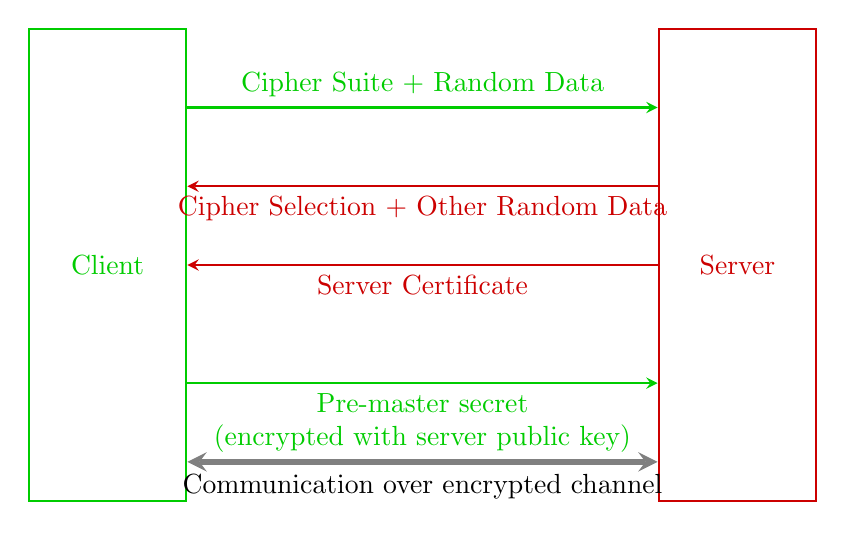
\begin{tikzpicture}[>=stealth, auto, node distance=5cm, thick]
        % Nodes
        \node[draw, green!80!black, minimum width=2cm, minimum height=6cm] (client) {Client};
        \node[draw, red!80!black, minimum width=2cm, minimum height=6cm, right of=client, node distance=8cm] (server) {Server};

        % Phase 1: Hello
        \draw[->, green!80!black] ([yshift=2cm]client.east) -- node[above] {Cipher Suite + Random Data} ([yshift=2cm]server.west);
        
        % Phase 2: Server response & Auth
        \draw[<-, red!80!black] ([yshift=1cm]client.east) -- node[below] {Cipher Selection + Other Random Data} ([yshift=1cm]server.west);
        \draw[<-, red!80!black] ([yshift=0cm]client.east) -- node[below] {Server Certificate} ([yshift=0cm]server.west);
        
        % Phase 3: Secret Transmission
        \draw[->, green!80!black] ([yshift=-1.5cm]client.east) -- node[below, align=center] {Pre-master secret \\ (encrypted with server public key)} ([yshift=-1.5cm]server.west);
        
        % Phase 4: Encrypted channel
        \draw[<->, gray, line width=2pt] ([yshift=-2.5cm]client.east) -- node[below, text=black] {Communication over encrypted channel} ([yshift=-2.5cm]server.west);
        
    \end{tikzpicture}
    \caption{Simplified TLS Handshake flow.}
    \label{fig:tls_handshake}
\end{figure}

\begin{enumerate}
    \item \textbf{Hello Phase:} The client sends the supported cipher suites and some random data. The server responds with the selected cipher suite and its own random data.
    \item \textbf{Server Authentication:} The server sends its X.509 digital certificate to the client. The client must verify this certificate:
    \begin{itemize}
        \item Is it within its validity period?
        \item Is the root Certificate Authority (CA) trusted by the OS/browser?
        \item Is the certificate mathematically valid (signature check)?
        \item Is it revoked (via CRL or OCSP)?
        \item Is the Common Name (or Subject Alternative Name) in the certificate exactly matching the requested domain?
    \end{itemize}
    
    \begin{tcolorbox}[colback=blue!5!white,colframe=blue!75!black,title=Exam Insight]
    Questions about this topic often involve analyzing PKI and Certificate practices. You might be asked to evaluate certificate validation steps, analyze different PKI architectures (e.g., graph vs. tree structures, mechanisms for air-gapped devices), or discuss the security implications of certificate lifetime reduction. Be prepared to explain how each step of validation prevents specific impersonation or MITM attacks.
    \end{tcolorbox}

    \item \textbf{Secret Transmission:} The client generates a \textit{pre-master secret}, encrypts it with the server's public key (extracted from the certificate), and sends it to the server. Only the legitimate server possessing the corresponding private key can decrypt this message.
    \item \textbf{Client Authentication (Optional):} If requested by the server, the client can also send its own certificate and prove possession of the private key by signing a piece of data (usually a hash of the previous handshake messages).
    \item \textbf{Secret Computation:} Both parties now independently compute the \textit{shared secret} (master secret) using the pre-master secret, the client's random data, and the server's random data.
    \item \textbf{Encrypted Communication Phase:} All subsequent communication is symmetrically encrypted and integrity-protected using keys derived from the shared master secret.
\end{enumerate}

\subsection{Resistance to Man-In-The-Middle (MITM) Attacks}
TLS is resistant to MITM attacks by design. Let's analyze what an attacker in the middle could attempt:
\begin{itemize}
    \item \textbf{Let the original certificate through:} The MITM intercepts the traffic but cannot decrypt the pre-master secret because they do not possess the server's private key. They can see the encrypted traffic but lack the shared master key.
    \item \textbf{Send a fake certificate (signed by a non-trusted CA):} The client's browser will reject it because the CA is not in its trusted root store.
    \item \textbf{Send a good certificate with a fake name:} The client will reject it because the requested domain name will not match the certificate's subject name.
    \item \textbf{Send a good certificate but substitute the public key:} This invalidates the CA's digital signature on the certificate, causing the client to reject it.
\end{itemize}

\subsection{TLS Pros and Cons}
\textbf{Pros:}
\begin{itemize}
    \item Protects transmissions (Confidentiality, Integrity).
    \item Ensures authentication of the server, and optionally the client.
\end{itemize}
\textbf{Cons:}
\begin{itemize}
    \item No protection before or after transmission: the data is plaintext on the server and on the client. A trojan on the client or a malicious merchant can still abuse the data.
    \item Relies heavily on the Public Key Infrastructure (PKI).
    \item It is not foolproof, especially regarding user interface and human factors.
\end{itemize}

\section{Security UI and SSL Stripping}
While the cryptographic protocol is secure, the user interface and human gullibility introduce vulnerabilities. 

\subsection{Social Engineering and Warnings}
In early browsers, invalid certificates resulted in a simple dialog box prompting the user ``Do you want to proceed? (Yes/No)''. Most users reflexively clicked ``Yes'' to access the content, entirely violating the assumptions of TLS and making MITM attacks successful. Modern browsers have evolved their UI to make bypassing security warnings much more difficult and scary, strongly advising users to ``Go Back''.

\subsection{SSL Stripping}
A classic attack is SSL Stripping. A victim attempts to connect to a website via plain HTTP (e.g., typing \texttt{bank.com} instead of \texttt{https://bank.com}). The MITM intercepts this HTTP request, establishes an HTTPS connection with the real server, but serves the victim a plain HTTP version of the site (or a fake login form posting to an HTTP endpoint). The user sees a normal page, unaware that the padlock is missing, and inputs their credentials.

\begin{tcolorbox}[colback=blue!5!white,colframe=blue!75!black,title=Exam Insight]
Questions about this topic usually ask you to propose network mitigations or topology changes to prevent specific attacks. You should be able to suggest protocols (such as VPN, HTTPS/HSTS, IPsec) or configurations (DMZ, NAT, Port Security) and evaluate the effectiveness of these countermeasures in defending against MITM, eavesdropping, and session hijacking after network changes have been made.
\end{tcolorbox}

\section{Overcoming TLS/PKI Limitations}
The security guarantees of TLS depend entirely on the security and trust of the root and intermediate CAs. CAs can generate certificates for any domain, and browsers inherently trust hundreds of CAs pre-installed by the OS or the browser vendor.

\subsection{CA Incidents}
History is rife with CA compromises and mis-issuances:
\begin{itemize}
    \item \textbf{2011 Diginotar:} Compromised, leading to rogue certificates for major domains (distrusted and collapsed).
    \item \textbf{2009-2015 Symantec:} Issued test certificates for existing domains like Google. Caught through CT logs, eventually distrusted.
    \item \textbf{2012 Trustwave:} Issued a MITM certificate for a corporate data loss prevention appliance.
\end{itemize}
Dropping a non-compliant CA is difficult because it instantly breaks access to thousands of legitimate websites using that CA.

\subsection{Defense Mechanisms}
To counter these systemic PKI weaknesses and attacks like SSL stripping, several mechanisms were introduced:

\begin{itemize}
    \item \textbf{HSTS (HTTP Strict Transport Security):} An HTTP header that tells the browser to \textit{always} connect to that domain using HTTPS. Browsers also implement an HSTS preload list, meaning the browser will outright refuse to load certain sites over plain HTTP even on the first visit. This effectively kills SSL stripping.
    \item \textbf{HPKP (HTTP Public Key Pinning):} An HTTP header that told the browser to ``pin'' a specific certificate or CA for a domain. If the site later presented a certificate from a different CA, the browser would refuse it. This defended against CA mis-issuance. However, it was \textbf{deprecated} because a simple configuration error (or a malicious ransom attack pinning an attacker's key) could render a website permanently inaccessible to its users.
    \item \textbf{Certificate Transparency (CT):} CAs must submit the metadata of every issued certificate to an independent, publicly auditable, append-only log. Browsers can enforce this by refusing certificates that lack proof of inclusion in a CT log. This allows site owners to monitor the logs (e.g., via \texttt{https://crt.sh}) and detect if any CA fraudulently issues a certificate for their domain.
\end{itemize}

\section{SET (Secure Electronic Transaction)}

\begin{tcolorbox}[colback=blue!5!white,colframe=blue!75!black,title=Exam Insight]
While SET is a legacy protocol, understanding its cryptographic protocol design (such as the dual signature) is highly relevant for exercises that ask you to analyze, prove the security/integrity of, or design custom secure cryptographic protocols. You may be asked to find vulnerabilities, propose fixes, or design protocols for confidentiality and integrity in specific scenarios (e.g., firmware updates, digitally controlled safes). Understanding how SET separates information without compromising integrity is a key pattern to study.
\end{tcolorbox}

Introduced by a joint effort from the VISA and MasterCard consortium, SET aimed to protect \textit{transactions}, not just connections. 

\subsection{The Approach}
In a standard HTTPS transaction, the user sends their credit card details directly to the merchant, who then forwards them to the payment gateway. The merchant sees the card details, creating a risk.
In SET, the cardholder sends:
\begin{itemize}
    \item The \textbf{order of goods} to the \textbf{merchant} only.
    \item The \textbf{payment data} to the \textbf{payment gateway} only.
\end{itemize}
The gateway is empowered to verify the correspondence between the order and the payment without revealing the card details to the merchant.

\subsection{Dual Signature}
SET uses the concept of a \textit{dual signature} to link two messages intended for two different recipients.

\begin{figure}[htpb]
    \centering
    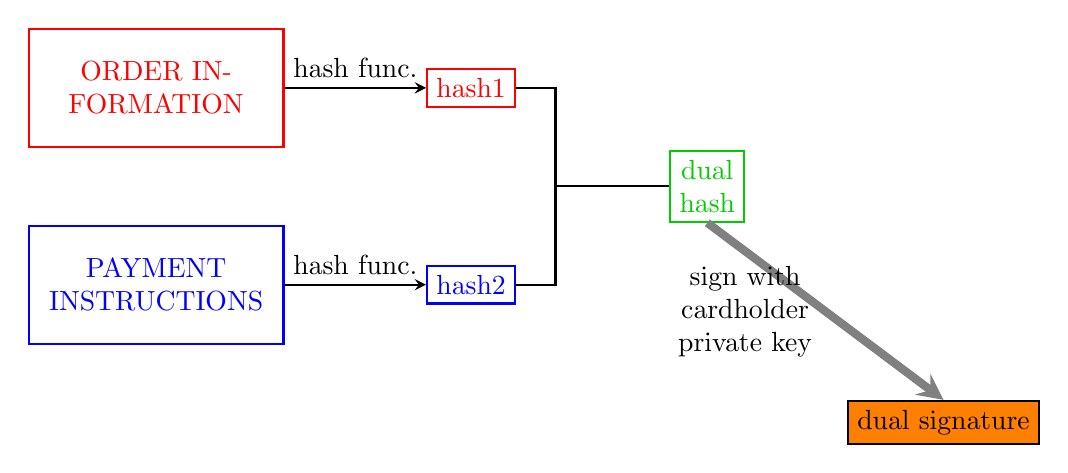
\begin{tikzpicture}[>=stealth, auto, node distance=2.5cm, thick]
        % Nodes
        \node[draw, red, text width=3cm, align=center, minimum height=1.5cm] (order) {ORDER INFORMATION};
        \node[draw, blue, text width=3cm, align=center, minimum height=1.5cm, below of=order] (payment) {PAYMENT INSTRUCTIONS};
        
        \node[draw, red, right of=order, node distance=4cm] (hash1) {hash1};
        \node[draw, blue, right of=payment, node distance=4cm] (hash2) {hash2};
        
        \node[draw, green!80!black, right of=hash1, yshift=-1.25cm, node distance=3cm, align=center] (dualhash) {dual\\hash};
        
        \node[draw, fill=orange, right of=dualhash, node distance=3cm, yshift=-3cm, align=center] (dualsig) {dual signature};

        % Edges
        \draw[->] (order) -- node[above] {hash func.} (hash1);
        \draw[->] (payment) -- node[above] {hash func.} (hash2);
        
        \draw[-] (hash1.east) -- ++(0.5,0) |- (dualhash.west);
        \draw[-] (hash2.east) -- ++(0.5,0) |- (dualhash.west);
        
        \draw[->, gray, line width=3pt] (dualhash.south) -- node[left, text=black, align=center] {sign with \\ cardholder \\ private key} (dualsig.north);
    \end{tikzpicture}
    \caption{Dual Signature Generation in SET.}
    \label{fig:dual_signature}
\end{figure}

The cardholder hashes the order information (\texttt{hash1}) and hashes the payment instructions (\texttt{hash2}). These two hashes are concatenated and hashed again to produce the \texttt{dual hash}. The cardholder then signs this \texttt{dual hash} with their private key, creating the \textit{dual signature}.

\subsection{Data Transmission and Verification}
The cardholder encrypts the order info, \texttt{hash2}, and the dual signature with the merchant's public key. Separately, they encrypt the payment instructions, \texttt{hash1}, and the dual signature with the payment gateway's public key.
\begin{itemize}
    \item \textbf{Merchant side verification:} The merchant decrypts their package, verifies the order, hashes the order info to recreate \texttt{hash1}. They then combine it with the provided \texttt{hash2} to compute the dual hash. Finally, they verify the dual signature using the cardholder's public key.
    \item \textbf{Payment gateway side verification:} The gateway does the perfect dual. It decrypts its package, hashes the payment instructions to recreate \texttt{hash2}, combines it with the provided \texttt{hash1}, computes the dual hash, and verifies the signature.
\end{itemize}

\subsection{Why did SET Fail?}
Despite its elegant cryptographic design, SET failed commercially. 
SET required a digital certificate from all three parties: the Merchant, the Payment Gateway, and the Cardholder. While issuing certificates to merchants and gateways is feasible, requiring every individual consumer to obtain, manage, and use a digital certificate simply \textbf{does not scale}. 
It required a cumbersome pre-registration process for the cardholder. This lack of transparency and steep learning curve meant it never reached critical mass. If a user had to go through a complex setup just to buy a book, they would abandon the purchase.
Nowadays, a simple HTTPS redirect to a bank's tokenized portal is commonly used, providing a transparent and secure user experience without the need for client-side PKI.

\section*{Chapter Summary}
This chapter explores the challenges of securing communications over the Internet, focusing on two major protocols: TLS (Transport Layer Security) and SET (Secure Electronic Transaction). It covers the mechanisms of the TLS handshake, its reliance on Public Key Infrastructure (PKI), and defense mechanisms against attacks like SSL Stripping (e.g., HSTS, Certificate Transparency). Furthermore, it discusses the SET protocol, its innovative use of dual signatures to separate order and payment information, and the reasons for its eventual commercial failure.

\begin{table}[htpb]
    \centering
    \renewcommand{\arraystretch}{1.3}
    \begin{tabular}{|l|p{10cm}|}
        \hline
        \textbf{Protocol} & \textbf{Key Characteristics} \\ \hline
        \textbf{TLS} & Evolved from SSL; provides confidentiality, integrity, and authentication; relies on PKI; vulnerable to CA compromises but mitigated by HSTS and CT. \\ \hline
        \textbf{SET} & Protects transactions rather than just connections; uses dual signatures; failed commercially due to poor scalability and lack of user transparency. \\ \hline
    \end{tabular}
    \caption{Comparison of Network Security Protocols}
    \label{tab:protocol_summary}
\end{table}


% Chapter 12: Malicious Software
\chapter{Malicious Software}
\label{ch:malicious_software}

\section{Introduction and Malware Categories}
The term \textbf{malware} is a portmanteau derived from the words \textit{malicious software}. Fundamentally, it refers to any executable code or script that is intentionally written to violate a security policy. Unlike software bugs or unintentional vulnerabilities, malware is designed with malicious intent to compromise the confidentiality, integrity, or availability of a system.

Rather than being a single, monolithic concept, malware encompasses several distinct categories, characterized primarily by how they spread and what features they offer to the attacker. The primary categories are:

\begin{itemize}
    \item \textbf{Viruses}: A virus is a piece of code that self-propagates by infecting executables or other files. Crucially, traditional viruses are \textit{not} standalone programs; they require a host file to operate. When the infected host program is executed, the virus code runs alongside it, allowing it to seek out and infect other files. Viruses can infect application executables, documents containing macros, and even boot loaders.
    \item \textbf{Worms}: Unlike viruses, worms are \textit{standalone} programs that self-propagate, often autonomously across networks. They do not need to attach themselves to an existing host file. Worms typically spread by exploiting vulnerabilities in network services on target hosts or by leveraging social engineering (e.g., mail worms that trick users into executing an attachment).
    \item \textbf{Trojan Horses}: A Trojan horse (or simply a Trojan) is a seemingly benign program that hides a hidden malicious functionality. Unlike viruses and worms, Trojans do not generally self-propagate. Their primary purpose is to deceive the user into installing them, after which they may establish a backdoor to allow remote control of the compromised system, steal information, or drop additional malware.
\end{itemize}

\section{The Malicious Code Lifecycle}
The lifecycle of typical malicious software can be broken down into four key phases: \textbf{Reproduce}, \textbf{Infect}, \textbf{Stay Hidden}, and \textbf{Run Payload}.

\subsection{Reproduction and Infection}
During the reproduction and infection phase, the malware must strike a delicate balance between maximizing its infection rate and minimizing its chances of detection. A rapid, aggressive infection strategy may spread the malware quickly but is highly noisy and likely to be detected by network intrusion detection systems or antivirus software. 

To infect other systems, malware needs to identify a suitable \textbf{propagation vector}. This vector may rely on social engineering (e.g., tricking a user into downloading an infected file) or vulnerability exploits (e.g., exploiting a buffer overflow in a remotely accessible network daemon). For viruses, this phase involves identifying suitable target files on the local file system and injecting the malicious code into them. 

It is important to note that most modern malware no longer relies heavily on automated self-propagation. Contemporary threats, such as botnet implants and banking Trojans, are primarily distributed via centralized exploit kits, malvertising campaigns, or spear-phishing emails, rather than spreading autonomously from host to host.

\subsection{Execution of the Payload}
The ultimate goal of the malware is to deliver its \textbf{payload}. The payload represents the actual malicious action the software is designed to perform. Historically, payloads were often designed simply to be annoying or to demonstrate the author's technical prowess. Examples of early annoying payloads include visual glitches like the ``ping-pong'' virus or the ``Cascade'' virus, which caused characters on a DOS terminal to fall to the bottom of the screen.

Today, payloads are almost exclusively designed for financial gain, espionage, or sabotage. Modern payloads include encrypting the filesystem for ransom (ransomware), installing keyloggers to steal banking credentials, or enrolling the infected machine into a botnet.

\section{Computer Viruses}

\subsection{A Brief History of Viruses}
The concept of self-replicating programs dates back to the early days of computing:
\begin{itemize}
    \item \textbf{1971 -- Creeper}: Often considered the first self-replicating program. It was an experimental program written for the PDP-10 operating system, famously displaying the message, ``I'm the creeper, catch me if you can!''
    \item \textbf{1981 -- Elk Cloner}: The first major outbreak of a virus in the wild. Written by a 15-year-old, it infected Apple II floppy disks and spread whenever a computer was booted from an infected disk.
    \item \textbf{1983 -- The first documented experimental virus}: Fred Cohen conducted pioneering academic work on computer viruses. The term ``computer virus'' was actually coined by his academic advisor, Len Adleman (the ``A'' in RSA cryptography).
\end{itemize}

\subsection{Theory of Computer Viruses}
In 1983, Fred Cohen theorized the existence of computer viruses and produced the first formal examples. From a theoretical computer science perspective, a virus is a fascinating implementation of self-modifying and self-propagating code.

Cohen's research formalized the security challenges posed by such software and led to a profound theoretical conclusion: \textbf{it is impossible to build a perfect virus detector}. This is a direct consequence of the halting problem and the undecidability of program behavior.

The proof sketch is as follows:
\begin{enumerate}
    \item Assume there exists a perfect detection program $P$ that can analyze any program and correctly output \texttt{True} if the program is a virus, and \texttt{False} otherwise.
    \item We can construct a malicious program $V$ that uses $P$ as a subroutine to analyze itself.
    \item $V$ operates with the following logic:
    \begin{itemize}
        \item If $P(V) = \texttt{True}$ (i.e., $P$ detects $V$ as a virus), $V$ immediately halts and does \textit{not} spread. Thus, $V$ did not exhibit viral behavior, meaning $P$ was wrong.
        \item If $P(V) = \texttt{False}$ (i.e., $P$ declares $V$ is not a virus), $V$ activates its propagation routine and spreads. Thus, $V$ is a virus, and $P$ was wrong again.
    \end{itemize}
\end{enumerate}
Because a perfect detector can be mathematically proven impossible, the cybersecurity industry must rely on imperfect heuristic, behavioral, and signature-based detection mechanisms.

\subsection{Infection Techniques}
Viruses have evolved various mechanisms for attaching themselves to host systems and files:

\paragraph{Boot Viruses}
These viruses target the startup sequence of a computer. They typically infect the Master Boot Record (MBR) of a hard disk (the very first sector) or the boot sector of individual partitions. Classic examples include the \textit{Brain} virus. While boot viruses became rare as operating systems matured, the interest in them has been renewed in recent years (e.g., Mebroot/Torpig) due to the rise of diskless workstations and virtual machines (e.g., the SubVirt academic proof-of-concept).

\paragraph{File Infectors}
File infectors target executable files. They can operate in several ways:
\begin{itemize}
    \item \textbf{Simple Overwrite Virus}: The simplest form, which blindly overwrites the beginning of the target executable with its own code. This destroys the original program, making the infection obvious as the host application will no longer function.
    \item \textbf{Parasitic Virus}: A more sophisticated approach where the virus appends its code to the end of the executable and modifies the program's original entry point to point to the viral code. After the virus runs, it typically passes control back to the original entry point, allowing the host application to run normally.
    \item \textbf{Cavity (or Multi-cavity) Virus}: These viruses attempt to keep the file size unchanged to avoid detection. They inject their code into unused regions (cavities or padding space) within the executable's structure.
\end{itemize}

\paragraph{Macro Viruses}
Traditionally, data files (like documents or images) were considered safe because they contained no executable code. However, the introduction of powerful macro languages (such as VBA in Microsoft Office) changed this paradigm. Macro functionalities allow executable code to be embedded directly within data files. For example, a spreadsheet macro can modify other spreadsheets, access the user's address book, and send emails. The most successful and famous example of this was the \textbf{Melissa virus} (1999), a large-scale email macro-virus that proved difficult to eradicate.

\section{Worms and the Evolution of Threats}

\subsection{A Brief History of Worms}
Worms represent a shift from local file infection to network-level self-propagation.
\begin{itemize}
    \item \textbf{1987 -- Christmas Worm}: A mass-mailer worm that hit IBM Mainframes, achieving 500,000 replications per hour and paralyzing many networks.
    \item \textbf{1988 -- The Internet Worm (Morris Worm)}: Created by Robert Morris Jr., a Ph.D. student at Cornell. Comprising only 99 lines of code, it brought down a significant portion of the early Internet (ARPANET). It connected to other computers, found and used vulnerabilities (e.g., a buffer overflow in \texttt{fingerd}, weak passwords), copied itself, and ran the copy. A flaw in the code caused it to re-infect machines in an infinite loop, causing severe resource exhaustion. The fallout led to the creation of CERT (Computer Emergency Response Team).
    \item \textbf{2000 -- ILOVEYOU}: A massive email worm relying heavily on social engineering, disguised as a love letter script (\texttt{LOVE-LETTER-FOR-YOU.txt.vbs}).
    \item \textbf{2001 -- Code Red}: A large-scale, exploit-based worm that was completely memory resident, leaving no files on the hard drive.
    \item \textbf{2003 -- SQL Slammer}: Known for its explosive growth rate, this worm propagated via a single UDP packet. Its small size allowed it to infect thousands of hosts in minutes.
\end{itemize}

\subsection{Modern Worms: Mass Scanners}
The basic pattern of a worm remains the same: infect a computer and seek out new targets. However, the speed and scale have increased dramatically, moving from hours to mere minutes to compromise hundreds of thousands of hosts. This speed is achieved through advanced scanning strategies:
\begin{itemize}
    \item \textbf{Random Address}: Probing randomly generated IP addresses.
    \item \textbf{Local Preference}: Weighting scans toward the local network subnet, which often has weaker internal firewalls and faster latency.
    \item \textbf{Permutation Scanning}: Dividing the entire IP address space among infected nodes to prevent multiple worms from scanning the same targets redundantly.
    \item \textbf{Hit List Scanning}: Pre-compiling a list of vulnerable targets before the worm is even launched, allowing the initial phase of the outbreak to be nearly instantaneous.
    \item \textbf{Warhol Worm}: A theoretical worm combining hit-list scanning for an explosive start and permutation scanning for rapid follow-up, designed to compromise the entire vulnerable Internet in 15 minutes.
\end{itemize}

\subsection{The ``Silence on the Wires'' and the Underground Economy}
In the early 2000s, security experts braced for continuous, massive worm outbreaks that could target critical Internet infrastructure. However, since 2004, there has been a noticeable ``silence on the wires.'' Major, self-propagating infrastructure-destroying worms largely disappeared. 

Why did the worm writers seemingly vanish? The answer lies in a shift in motivation. Early hackers sought notoriety and disruption. However, modern attackers are motivated by \textbf{monetization}. If a worm brings down the Internet infrastructure, the attackers lose the very platform they need to communicate with their compromised hosts and generate profit.

This shift gave rise to a sophisticated underground cybercrime economy. Attackers focus on direct monetization (abusing credit cards, premium rate numbers) and indirect monetization (information gathering, renting out botnet infrastructure). 

\section{Botnets and the Cybercrime Ecosystem}

\subsection{Rise of the Bots}
The term \textit{bot} originated from IRC (Internet Relay Chat) networks, where automated scripts provided useful channel management services. However, malicious actors began abusing IRC bots to coordinate attacks, leading to the first documented Distributed Denial of Service (DDoS) ``IRCwars.''

By 1999, tools like \textit{trinoo} were released, allowing for coordinated DDoS attacks from multiple compromised machines. In the early 2000s, massive DDoS attacks against high-profile websites (Amazon, CNN, eBay) garnered widespread media coverage, demonstrating the power of distributed computing turned malicious.

\subsection{Botnet Architecture and Capabilities}
A \textbf{botnet} is a network of compromised machines (bots or zombies) controlled centrally by an attacker known as the \textbf{botmaster} or botherder.

\begin{figure}[htbp]
    \centering
    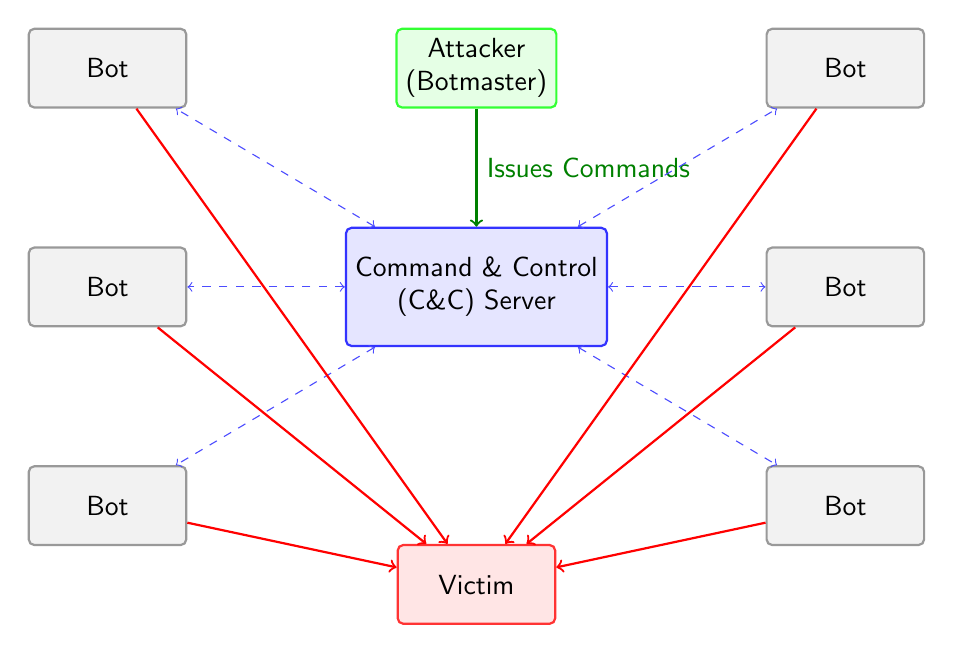
\begin{tikzpicture}[
        node distance=1.5cm and 2cm,
        every node/.style={align=center, font=\sffamily},
        bot/.style={rectangle, draw=gray!80, thick, fill=gray!10, minimum width=2cm, minimum height=1cm, rounded corners=2pt},
        cnc/.style={rectangle, draw=blue!80, thick, fill=blue!10, minimum width=2.5cm, minimum height=1.5cm, rounded corners=2pt},
        attacker/.style={rectangle, draw=green!80, thick, fill=green!10, minimum width=2cm, minimum height=1cm, rounded corners=2pt},
        victim/.style={rectangle, draw=red!80, thick, fill=red!10, minimum width=2cm, minimum height=1cm, rounded corners=2pt}
    ]
        % Nodes
        \node[cnc] (cnc) {Command \& Control\\(C\&C) Server};
        \node[attacker, above=of cnc] (attacker) {Attacker\\(Botmaster)};
        
        \node[bot, above left=of cnc] (bot1) {Bot};
        \node[bot, left=of cnc] (bot2) {Bot};
        \node[bot, below left=of cnc] (bot3) {Bot};
        
        \node[bot, above right=of cnc] (bot4) {Bot};
        \node[bot, right=of cnc] (bot5) {Bot};
        \node[bot, below right=of cnc] (bot6) {Bot};
        
        \node[victim, below=of cnc, yshift=-1cm] (victim) {Victim};
        
        % Connections
        \draw[->, thick, green!50!black] (attacker) -- (cnc) node[midway, right] {Issues Commands};
        
        \draw[<->, dashed, blue!70] (cnc) -- (bot1);
        \draw[<->, dashed, blue!70] (cnc) -- (bot2);
        \draw[<->, dashed, blue!70] (cnc) -- (bot3);
        \draw[<->, dashed, blue!70] (cnc) -- (bot4);
        \draw[<->, dashed, blue!70] (cnc) -- (bot5);
        \draw[<->, dashed, blue!70] (cnc) -- (bot6);
        
        \draw[->, thick, red] (bot1) -- (victim);
        \draw[->, thick, red] (bot2) -- (victim);
        \draw[->, thick, red] (bot3) -- (victim);
        \draw[->, thick, red] (bot4) -- (victim);
        \draw[->, thick, red] (bot5) -- (victim);
        \draw[->, thick, red] (bot6) -- (victim);
        
    \end{tikzpicture}
    \caption{Typical Botnet Architecture. The botmaster uses a C\&C server to issue commands to a large network of infected hosts, which then carry out coordinated attacks against a victim.}
    \label{fig:botnet}
\end{figure}

The communication between the bots and the botmaster relies on Command and Control (C\&C) channels, which can use IRC, HTTP, P2P networks, or custom protocols. Modern bots are highly sophisticated platforms. For instance, an analysis of the \textit{Phatbot} malware revealed capabilities such as harvesting email addresses, logging keypresses, sniffing network traffic, taking screenshots, setting up SOCKS proxies for spamming, stealing Windows CD keys, downloading additional files, and even killing rival malware and AV processes. A key feature of modern bots is their ability to self-update, allowing the botmaster to change the bot's functionality entirely post-infection.

\subsection{Threats Posed by Botnets}
Botnets pose severe threats on two fronts:
\begin{enumerate}
    \item \textbf{For the infected host}: Complete loss of privacy and data security. The bot will harvest identity data, financial credentials, private files, and email address books.
    \item \textbf{For the rest of the Internet}: The infected machine becomes a weapon. It will be used for spamming, participating in DDoS attacks, propagating network worms, or acting as support infrastructure for illegal activities (e.g., hosting phishing sites or drive-by-download servers).
\end{enumerate}

The cybercrime ecosystem has evolved into organized groups offering "Exploit-as-a-Service," exploit development, site infection, and victim monitoring. Since 2010, the landscape has further expanded to include high-profile targets, critical infrastructure attacks (e.g., Stuxnet), state-sponsored espionage, and the devastating rise of Ransomware (e.g., CryptoLocker, WannaCry).

\section{Stealth Techniques: Obfuscation, Metamorphism, and Packing}

\begin{tcolorbox}[colback=blue!5!white,colframe=blue!75!black,title=Exam Insight]
Expect questions asking you to identify evasive techniques directly from assembly or pseudo-code. You should be able to recognize polymorphic and metamorphic behavior, packing routines, anti-debugging tricks, dormant or event-triggered code, and time-bombs. You may also be asked to identify flaws in poorly implemented anti-analysis techniques—be prepared to explain how a defender could exploit these flaws to analyze the malware, or conversely, how to fix the flaw from an attacker's perspective. Another typical task is modifying assembly code to bypass signature matching, for example, by manually applying metamorphic transformations like dead code insertion, instruction reordering, or register swapping.
\end{tcolorbox}

As malware analysis techniques improved, malware authors developed sophisticated stealth techniques to evade detection and hinder reverse engineering.

\subsection{Entry Point Obfuscation}
Antivirus scanners historically sought malicious signatures near the entry point of an executable. Malware authors countered with \textbf{Entry Point Obfuscation} (EPO). Instead of modifying the main entry point, the virus hijacks control \textit{later} in the program's execution. This is achieved by overwriting function call instructions deep within the code or modifying import table addresses so that legitimate library calls are redirected to the malware.

\subsection{Polymorphism and Metamorphism}
To defeat signature-based detection, malware must change its appearance without altering its fundamental behavior.

\paragraph{Polymorphism}
Polymorphic malware encrypts or packs its main payload. The only visible code is a small decryption routine. With each new infection, the malware encrypts the payload using a different key, changing the bulk of the file's signature. However, the decryption routine itself remains constant (or slightly varied), which antivirus scanners can sometimes detect.

\paragraph{Metamorphism}
Metamorphic malware represents the pinnacle of obfuscation. It does not simply encrypt its payload; it rewrites its own code entirely for each infection. The \textit{syntax} of the code changes, but the \textit{semantics} (the actual behavior) are preserved. This is achieved through complex internal engines that utilize techniques like:
\begin{itemize}
    \item \textbf{Dead code insertion}: Inserting junk instructions (e.g., \texttt{NOP}, or paired instructions like \texttt{inc eax} followed by \texttt{dec eax}) that change the binary signature without affecting the program state.
    \item \textbf{Instruction reordering}: Changing the sequence of independent instructions.
    \item \textbf{Register swapping}: Systematically swapping the use of general-purpose registers throughout a function.
\end{itemize}

\subsection{Anti-virtualization and Packing}
Modern malware often assumes it might be executed in a security researcher's sandbox or an automated antivirus analysis engine. Consequently, malware actively checks its execution environment. If it detects that it is running inside a Virtual Machine (e.g., VMware, VirtualBox) or an emulator, it may terminate itself or exhibit benign behavior (a ``dormant period'') to avoid yielding useful analysis data.

Detection mechanisms rely on timing discrepancies (since virtualization adds overhead), identifying specific environment artifacts (e.g., specific MAC addresses, VM-specific drivers), or uncovering incomplete instruction set implementations in software emulators.

Furthermore, \textbf{Packing} is used to compress and encrypt the malicious payload. The packer extracts the payload dynamically in memory during execution. Advanced packers include metamorphic components, anti-debugging tricks, anti-VM checks, and code virtualization (compiling the malware into a custom bytecode that is interpreted by an embedded, custom virtual machine).

\section{Malware Analysis and Detection}

\begin{tcolorbox}[colback=blue!5!white,colframe=blue!75!black,title=Exam Insight]
A frequent exam scenario requires discussing whether \textbf{Static} or \textbf{Dynamic} analysis is more appropriate for a given malware sample. You must detail the key elements to observe in each method (e.g., full code visibility vs. runtime artifacts). Furthermore, you should be ready to contrast \textbf{signature-based detection} with \textbf{heuristics}, describing their fundamental differences and limitations. Be prepared to explain how signature-based detection can be bypassed (e.g., through metamorphism) and how heuristics can be used to identify structural anomalies or suspicious behaviors that signatures might miss.
\end{tcolorbox}

\subsection{Defending Against Malware}
The primary defense against worms is \textbf{patching}, as worms rely heavily on exploiting known, unpatched vulnerabilities. Beyond patching, defense relies on detecting the malware via Antivirus/Anti-malware software using several strategies:
\begin{itemize}
    \item \textbf{Signatures}: A database of byte-level or instruction-level patterns that uniquely identify known malware. This approach is fast but utterly useless against zero-day threats or heavily metamorphic code.
    \item \textbf{Heuristics}: Checking for structural signs of infection without relying on specific patterns. Examples include checking if execution starts in the last section of the PE file, looking for incorrect PE header sizes, or identifying patched import address tables.
    \item \textbf{Behavioral Detection}: Monitoring the program at runtime for known malicious actions, such as unwarranted file encryption, injecting code into other processes, or making unauthorized registry changes.
\end{itemize}

\subsection{Static and Dynamic Analysis}
When a suspicious file is discovered, security analysts (or automated systems) employ two main analysis workflows:

\begin{itemize}
    \item \textbf{Static Analysis}: Parsing and examining the binary code \textit{without} executing it. Techniques include disassembly, decompilation, string extraction, and control-flow graph analysis.
    \begin{itemize}
        \item \textit{Pros}: Provides full code visibility, including dormant or unreachable logic. It is completely safe since the code is not executed.
        \item \textit{Cons}: Heavily hindered by obfuscation, metamorphism, and packing. Analysts must manually unpack and deobfuscate the code.
    \end{itemize}
    \item \textbf{Dynamic Analysis}: Executing the malware in a strictly controlled environment (sandbox) to monitor its behavior. Techniques include API hooking, tracing, and network monitoring.
    \begin{itemize}
        \item \textit{Pros}: Bypasses obfuscation completely; regardless of how the code is packed on disk, it must unpack itself in memory to execute. It easily reveals runtime artifacts (dropped files, network C\&C connections).
        \item \textit{Cons}: Limited code coverage (dormant branches or logic triggered only on specific dates won't execute). Carries the risk of the malware detecting the sandbox and halting its malicious activity.
    \end{itemize}
\end{itemize}

\section{Rootkits}

\subsection{Definition and Goals}
The term \textbf{rootkit} historically comes from the Unix world, referring to a ``kit'' of modified administrative tools planted by an attacker after gaining ``root'' (administrator) access. The primary goal of a rootkit is stealth: it aims to maintain the attacker's privileged access while making files, processes, users, network connections, and directories invisible to the system administrator.

\subsection{Userland vs. Kernel Space Rootkits}
Rootkits generally operate at one of two levels:

\paragraph{Userland Rootkits}
These operate at the application layer. In Unix environments, this involves replacing standard utilities (like \texttt{ps}, \texttt{netstat}, \texttt{ls}, \texttt{sshd}) with trojaned versions that filter out the attacker's artifacts. On Windows, this involves hooking APIs in user-space to hide processes from the Task Manager or Process Explorer. Userland rootkits are generally easier to build but are often incomplete and relatively easy to detect using cross-layer examination (e.g., comparing the output of a potentially trojaned \texttt{ps} command against a known-clean static binary).

\paragraph{Kernel Space Rootkits}
These are vastly more dangerous because they operate at Ring 0, modifying the core of the operating system itself. A kernel rootkit can intercept and alter data before it ever reaches userland applications, making standard security tools fundamentally untrustworthy.

The classic mechanism for a kernel rootkit is \textbf{Syscall Hijacking}. By modifying the System Call Table, an attacker intercepts requests from userland (e.g., a request to list directory contents via \texttt{sys\_getdents}). The rootkit's malicious routine executes first, queries the real operating system, filters out the malicious files from the results, and returns the sanitized list to the userland application.

Other kernel techniques include Direct Kernel Object Manipulation (DKOM), detour patching of kernel functions, and modifying the Interrupt Descriptor Table (IDT).

\subsection{Methods for Recognizing Rootkits}
Because a rootkit subverts the OS, querying the OS to find the rootkit is unreliable. Detection methods include:
\begin{itemize}
    \item \textbf{Cross-layer examination}: Comparing the high-level API view of the system against a lower-level view (e.g., comparing the list of files reported by the Windows API against raw NTFS volume parsing). Discrepancies indicate hidden items.
    \item \textbf{Post-mortem analysis}: Booting the system from a trusted, clean operating system (like a Live CD) and scanning the offline hard drive. Because the rootkit is not running in memory, it cannot hide its files.
    \item \textbf{Trusted Computing Base / Tripwire}: Monitoring cryptographic hashes of critical system binaries to detect unauthorized modifications.
\end{itemize}

\subsection{Advanced Rootkit Targets}
Rootkit technology continues to evolve, moving even lower in the hardware stack to ensure persistence. Advanced concepts include:
\begin{itemize}
    \item \textbf{BIOS/UEFI Rootkits}: Malware residing in the motherboard firmware, ensuring reinfection even if the hard drive is completely wiped and the OS is reinstalled.
    \item \textbf{Firmware Rootkits}: Infecting the firmware of peripheral devices, such as Network Interface Cards (NICs) or video cards.
    \item \textbf{Virtualization Rootkits}: A rootkit that loads itself as a hypervisor, pushing the legitimate operating system down into a virtual machine. From this position, the rootkit has absolute, invisible control over the entire OS.
\end{itemize}

\begin{tcolorbox}[colback=blue!5!white,colframe=blue!75!black,title=Chapter Summary]
This chapter covers malicious software, focusing on its lifecycle, types, and the constant arms race between attackers and defenders. It details computer viruses, worms, botnets, and rootkits. Crucially, it explores stealth techniques such as polymorphism and metamorphism, and contrasts static and dynamic malware analysis.
\end{tcolorbox}

\begin{table}[htbp]
\centering
\renewcommand{\arraystretch}{1.3}
\begin{tabular}{|l|p{10cm}|}
\hline
\textbf{Topic} & \textbf{Key Concepts} \\
\hline
Malware Categories & Viruses (host-dependent), Worms (standalone), Trojans (hidden malicious functionality) \\
Stealth Techniques & Obfuscation, Polymorphism (payload encryption), Metamorphism (code rewriting), Packing, Anti-virtualization \\
Analysis Methods & Static (examining code without execution), Dynamic (sandboxed execution) \\
Rootkits & Userland vs. Kernel Space (e.g., Syscall Hijacking), Evasion techniques \\
\hline
\end{tabular}
\caption{Overview of key concepts in malicious software.}
\label{tab:malware_summary}
\end{table}


\end{document}
